\documentclass[twoside]{book}

% Packages required by doxygen
\usepackage{fixltx2e}
\usepackage{calc}
\usepackage{doxygen}
\usepackage[export]{adjustbox} % also loads graphicx
\usepackage{graphicx}
\usepackage[utf8]{inputenc}
\usepackage{makeidx}
\usepackage{multicol}
\usepackage{multirow}
\PassOptionsToPackage{warn}{textcomp}
\usepackage{textcomp}
\usepackage[nointegrals]{wasysym}
\usepackage[table]{xcolor}

% Font selection
\usepackage[T1]{fontenc}
\usepackage[scaled=.90]{helvet}
\usepackage{courier}
\usepackage{amssymb}
\usepackage{sectsty}
\renewcommand{\familydefault}{\sfdefault}
\allsectionsfont{%
  \fontseries{bc}\selectfont%
  \color{darkgray}%
}
\renewcommand{\DoxyLabelFont}{%
  \fontseries{bc}\selectfont%
  \color{darkgray}%
}
\newcommand{\+}{\discretionary{\mbox{\scriptsize$\hookleftarrow$}}{}{}}

% Page & text layout
\usepackage{geometry}
\geometry{%
  a4paper,%
  top=2.5cm,%
  bottom=2.5cm,%
  left=2.5cm,%
  right=2.5cm%
}
\tolerance=750
\hfuzz=15pt
\hbadness=750
\setlength{\emergencystretch}{15pt}
\setlength{\parindent}{0cm}
\setlength{\parskip}{3ex plus 2ex minus 2ex}
\makeatletter
\renewcommand{\paragraph}{%
  \@startsection{paragraph}{4}{0ex}{-1.0ex}{1.0ex}{%
    \normalfont\normalsize\bfseries\SS@parafont%
  }%
}
\renewcommand{\subparagraph}{%
  \@startsection{subparagraph}{5}{0ex}{-1.0ex}{1.0ex}{%
    \normalfont\normalsize\bfseries\SS@subparafont%
  }%
}
\makeatother

% Headers & footers
\usepackage{fancyhdr}
\pagestyle{fancyplain}
\fancyhead[LE]{\fancyplain{}{\bfseries\thepage}}
\fancyhead[CE]{\fancyplain{}{}}
\fancyhead[RE]{\fancyplain{}{\bfseries\leftmark}}
\fancyhead[LO]{\fancyplain{}{\bfseries\rightmark}}
\fancyhead[CO]{\fancyplain{}{}}
\fancyhead[RO]{\fancyplain{}{\bfseries\thepage}}
\fancyfoot[LE]{\fancyplain{}{}}
\fancyfoot[CE]{\fancyplain{}{}}
\fancyfoot[RE]{\fancyplain{}{\bfseries\scriptsize Generated by Doxygen }}
\fancyfoot[LO]{\fancyplain{}{\bfseries\scriptsize Generated by Doxygen }}
\fancyfoot[CO]{\fancyplain{}{}}
\fancyfoot[RO]{\fancyplain{}{}}
\renewcommand{\footrulewidth}{0.4pt}
\renewcommand{\chaptermark}[1]{%
  \markboth{#1}{}%
}
\renewcommand{\sectionmark}[1]{%
  \markright{\thesection\ #1}%
}

% Indices & bibliography
\usepackage{natbib}
\usepackage[titles]{tocloft}
\setcounter{tocdepth}{3}
\setcounter{secnumdepth}{5}
\makeindex

% Hyperlinks (required, but should be loaded last)
\usepackage{ifpdf}
\ifpdf
  \usepackage[pdftex,pagebackref=true]{hyperref}
\else
  \usepackage[ps2pdf,pagebackref=true]{hyperref}
\fi
\hypersetup{%
  colorlinks=true,%
  linkcolor=blue,%
  citecolor=blue,%
  unicode%
}

% Custom commands
\newcommand{\clearemptydoublepage}{%
  \newpage{\pagestyle{empty}\cleardoublepage}%
}

\usepackage{caption}
\captionsetup{labelsep=space,justification=centering,font={bf},singlelinecheck=off,skip=4pt,position=top}

%===== C O N T E N T S =====

\begin{document}

% Titlepage & ToC
\hypersetup{pageanchor=false,
             bookmarksnumbered=true,
             pdfencoding=unicode
            }
\pagenumbering{alph}
\begin{titlepage}
\vspace*{7cm}
\begin{center}%
{\Large My Project }\\
\vspace*{1cm}
{\large Generated by Doxygen 1.8.13}\\
\end{center}
\end{titlepage}
\clearemptydoublepage
\pagenumbering{roman}
\tableofcontents
\clearemptydoublepage
\pagenumbering{arabic}
\hypersetup{pageanchor=true}

%--- Begin generated contents ---
\chapter{Hierarchical Index}
\section{Class Hierarchy}
This inheritance list is sorted roughly, but not completely, alphabetically\+:\begin{DoxyCompactList}
\item \contentsline{section}{ante\+:\+:Argument}{\pageref{structante_1_1Argument}}{}
\item \contentsline{section}{yy\+:\+:parser\+:\+:basic\+\_\+symbol$<$ by\+\_\+state $>$}{\pageref{structyy_1_1parser_1_1basic__symbol}}{}
\item \contentsline{section}{yy\+:\+:parser\+:\+:by\+\_\+type}{\pageref{structyy_1_1parser_1_1by__type}}{}
\item \contentsline{section}{ante\+:\+:Compiler}{\pageref{structante_1_1Compiler}}{}
\item \contentsline{section}{ante\+:\+:Compiler\+Args}{\pageref{structante_1_1CompilerArgs}}{}
\item \contentsline{section}{ante\+:\+:Compiler\+Ctxt}{\pageref{structante_1_1CompilerCtxt}}{}
\item \contentsline{section}{ante\+:\+:Ct\+Error}{\pageref{structante_1_1CtError}}{}
\begin{DoxyCompactList}
\item \contentsline{section}{ante\+:\+:Compilation\+Error}{\pageref{structante_1_1CompilationError}}{}
\item \contentsline{section}{ante\+:\+:Incomplete\+Type\+Error}{\pageref{structante_1_1IncompleteTypeError}}{}
\item \contentsline{section}{ante\+:\+:Type\+Var\+Error}{\pageref{structante_1_1TypeVarError}}{}
\end{DoxyCompactList}
\item \contentsline{section}{Ct\+Func}{\pageref{structCtFunc}}{}
\item \contentsline{section}{Data\+Type}{\pageref{structDataType}}{}
\item \contentsline{section}{Func\+Decl}{\pageref{structFuncDecl}}{}
\item \contentsline{section}{ante\+:\+:lazy\+\_\+printer}{\pageref{structante_1_1lazy__printer}}{}
\item \contentsline{section}{ante\+:\+:lazy\+\_\+str}{\pageref{structante_1_1lazy__str}}{}
\item \contentsline{section}{ante\+:\+:Lexer}{\pageref{classante_1_1Lexer}}{}
\item \contentsline{section}{yy\+:\+:location}{\pageref{classyy_1_1location}}{}
\item \contentsline{section}{ante\+:\+:Module}{\pageref{structante_1_1Module}}{}
\item \contentsline{section}{Node}{\pageref{structNode}}{}
\begin{DoxyCompactList}
\item \contentsline{section}{Array\+Node}{\pageref{structArrayNode}}{}
\item \contentsline{section}{Bin\+Op\+Node}{\pageref{structBinOpNode}}{}
\item \contentsline{section}{Block\+Node}{\pageref{structBlockNode}}{}
\item \contentsline{section}{Bool\+Lit\+Node}{\pageref{structBoolLitNode}}{}
\item \contentsline{section}{Char\+Lit\+Node}{\pageref{structCharLitNode}}{}
\item \contentsline{section}{Ext\+Node}{\pageref{structExtNode}}{}
\item \contentsline{section}{Flt\+Lit\+Node}{\pageref{structFltLitNode}}{}
\item \contentsline{section}{Global\+Node}{\pageref{structGlobalNode}}{}
\item \contentsline{section}{If\+Node}{\pageref{structIfNode}}{}
\item \contentsline{section}{Import\+Node}{\pageref{structImportNode}}{}
\item \contentsline{section}{Int\+Lit\+Node}{\pageref{structIntLitNode}}{}
\item \contentsline{section}{Jump\+Node}{\pageref{structJumpNode}}{}
\item \contentsline{section}{Let\+Binding\+Node}{\pageref{structLetBindingNode}}{}
\item \contentsline{section}{Match\+Branch\+Node}{\pageref{structMatchBranchNode}}{}
\item \contentsline{section}{Match\+Node}{\pageref{structMatchNode}}{}
\item \contentsline{section}{Mod\+Node}{\pageref{structModNode}}{}
\item \contentsline{section}{Named\+Val\+Node}{\pageref{structNamedValNode}}{}
\item \contentsline{section}{Parent\+Node}{\pageref{structParentNode}}{}
\begin{DoxyCompactList}
\item \contentsline{section}{Data\+Decl\+Node}{\pageref{structDataDeclNode}}{}
\item \contentsline{section}{For\+Node}{\pageref{structForNode}}{}
\item \contentsline{section}{Func\+Decl\+Node}{\pageref{structFuncDeclNode}}{}
\item \contentsline{section}{Trait\+Node}{\pageref{structTraitNode}}{}
\item \contentsline{section}{While\+Node}{\pageref{structWhileNode}}{}
\end{DoxyCompactList}
\item \contentsline{section}{Pre\+Proc\+Node}{\pageref{structPreProcNode}}{}
\item \contentsline{section}{Ret\+Node}{\pageref{structRetNode}}{}
\item \contentsline{section}{Root\+Node}{\pageref{structRootNode}}{}
\item \contentsline{section}{Str\+Lit\+Node}{\pageref{structStrLitNode}}{}
\item \contentsline{section}{Tuple\+Node}{\pageref{structTupleNode}}{}
\item \contentsline{section}{Type\+Cast\+Node}{\pageref{structTypeCastNode}}{}
\item \contentsline{section}{Type\+Node}{\pageref{structTypeNode}}{}
\item \contentsline{section}{Un\+Op\+Node}{\pageref{structUnOpNode}}{}
\item \contentsline{section}{Var\+Assign\+Node}{\pageref{structVarAssignNode}}{}
\item \contentsline{section}{Var\+Decl\+Node}{\pageref{structVarDeclNode}}{}
\item \contentsline{section}{Var\+Node}{\pageref{structVarNode}}{}
\end{DoxyCompactList}
\item \contentsline{section}{Node\+Iterator}{\pageref{structNodeIterator}}{}
\item \contentsline{section}{yy\+:\+:parser}{\pageref{classyy_1_1parser}}{}
\item \contentsline{section}{yy\+:\+:position}{\pageref{classyy_1_1position}}{}
\item runtime\+\_\+error\begin{DoxyCompactList}
\item \contentsline{section}{yy\+:\+:parser\+:\+:syntax\+\_\+error}{\pageref{structyy_1_1parser_1_1syntax__error}}{}
\end{DoxyCompactList}
\item \contentsline{section}{yy\+:\+:slice$<$ T, S $>$}{\pageref{classyy_1_1slice}}{}
\item \contentsline{section}{yy\+:\+:stack$<$ T, S $>$}{\pageref{classyy_1_1stack}}{}
\item \contentsline{section}{yy\+:\+:stack$<$ stack\+\_\+symbol\+\_\+type $>$}{\pageref{classyy_1_1stack}}{}
\item \contentsline{section}{yy\+:\+:parser\+:\+:token}{\pageref{structyy_1_1parser_1_1token}}{}
\item \contentsline{section}{Trait}{\pageref{structTrait}}{}
\item \contentsline{section}{Type\+Check\+Result}{\pageref{structTypeCheckResult}}{}
\item \contentsline{section}{Typed\+Value}{\pageref{structTypedValue}}{}
\begin{DoxyCompactList}
\item \contentsline{section}{Method\+Val}{\pageref{structMethodVal}}{}
\end{DoxyCompactList}
\item \contentsline{section}{Union\+Tag}{\pageref{structUnionTag}}{}
\item \contentsline{section}{Variable}{\pageref{structVariable}}{}
\item Base\begin{DoxyCompactList}
\item \contentsline{section}{yy\+:\+:parser\+:\+:basic\+\_\+symbol$<$ Base $>$}{\pageref{structyy_1_1parser_1_1basic__symbol}}{}
\end{DoxyCompactList}
\end{DoxyCompactList}

\chapter{Class Index}
\section{Class List}
Here are the classes, structs, unions and interfaces with brief descriptions\+:\begin{DoxyCompactList}
\item\contentsline{section}{\hyperlink{structante_1_1Argument}{ante\+::\+Argument} }{\pageref{structante_1_1Argument}}{}
\item\contentsline{section}{\hyperlink{structArrayNode}{Array\+Node} }{\pageref{structArrayNode}}{}
\item\contentsline{section}{\hyperlink{structyy_1_1parser_1_1basic__symbol}{yy\+::parser\+::basic\+\_\+symbol$<$ Base $>$} }{\pageref{structyy_1_1parser_1_1basic__symbol}}{}
\item\contentsline{section}{\hyperlink{structBinOpNode}{Bin\+Op\+Node} }{\pageref{structBinOpNode}}{}
\item\contentsline{section}{\hyperlink{structBlockNode}{Block\+Node} }{\pageref{structBlockNode}}{}
\item\contentsline{section}{\hyperlink{structBoolLitNode}{Bool\+Lit\+Node} }{\pageref{structBoolLitNode}}{}
\item\contentsline{section}{\hyperlink{structyy_1_1parser_1_1by__type}{yy\+::parser\+::by\+\_\+type} \\*Type access provider for token (enum) based symbols }{\pageref{structyy_1_1parser_1_1by__type}}{}
\item\contentsline{section}{\hyperlink{structCharLitNode}{Char\+Lit\+Node} }{\pageref{structCharLitNode}}{}
\item\contentsline{section}{\hyperlink{structante_1_1CompilationError}{ante\+::\+Compilation\+Error} }{\pageref{structante_1_1CompilationError}}{}
\item\contentsline{section}{\hyperlink{structante_1_1Compiler}{ante\+::\+Compiler} }{\pageref{structante_1_1Compiler}}{}
\item\contentsline{section}{\hyperlink{structante_1_1CompilerArgs}{ante\+::\+Compiler\+Args} }{\pageref{structante_1_1CompilerArgs}}{}
\item\contentsline{section}{\hyperlink{structante_1_1CompilerCtxt}{ante\+::\+Compiler\+Ctxt} }{\pageref{structante_1_1CompilerCtxt}}{}
\item\contentsline{section}{\hyperlink{structante_1_1CtError}{ante\+::\+Ct\+Error} }{\pageref{structante_1_1CtError}}{}
\item\contentsline{section}{\hyperlink{structCtFunc}{Ct\+Func} }{\pageref{structCtFunc}}{}
\item\contentsline{section}{\hyperlink{structDataDeclNode}{Data\+Decl\+Node} }{\pageref{structDataDeclNode}}{}
\item\contentsline{section}{\hyperlink{structDataType}{Data\+Type} }{\pageref{structDataType}}{}
\item\contentsline{section}{\hyperlink{structExtNode}{Ext\+Node} }{\pageref{structExtNode}}{}
\item\contentsline{section}{\hyperlink{structFltLitNode}{Flt\+Lit\+Node} }{\pageref{structFltLitNode}}{}
\item\contentsline{section}{\hyperlink{structForNode}{For\+Node} }{\pageref{structForNode}}{}
\item\contentsline{section}{\hyperlink{structFuncDecl}{Func\+Decl} }{\pageref{structFuncDecl}}{}
\item\contentsline{section}{\hyperlink{structFuncDeclNode}{Func\+Decl\+Node} }{\pageref{structFuncDeclNode}}{}
\item\contentsline{section}{\hyperlink{structGlobalNode}{Global\+Node} }{\pageref{structGlobalNode}}{}
\item\contentsline{section}{\hyperlink{structIfNode}{If\+Node} }{\pageref{structIfNode}}{}
\item\contentsline{section}{\hyperlink{structImportNode}{Import\+Node} }{\pageref{structImportNode}}{}
\item\contentsline{section}{\hyperlink{structante_1_1IncompleteTypeError}{ante\+::\+Incomplete\+Type\+Error} }{\pageref{structante_1_1IncompleteTypeError}}{}
\item\contentsline{section}{\hyperlink{structIntLitNode}{Int\+Lit\+Node} }{\pageref{structIntLitNode}}{}
\item\contentsline{section}{\hyperlink{structJumpNode}{Jump\+Node} }{\pageref{structJumpNode}}{}
\item\contentsline{section}{\hyperlink{structante_1_1lazy__printer}{ante\+::lazy\+\_\+printer} }{\pageref{structante_1_1lazy__printer}}{}
\item\contentsline{section}{\hyperlink{structante_1_1lazy__str}{ante\+::lazy\+\_\+str} }{\pageref{structante_1_1lazy__str}}{}
\item\contentsline{section}{\hyperlink{structLetBindingNode}{Let\+Binding\+Node} }{\pageref{structLetBindingNode}}{}
\item\contentsline{section}{\hyperlink{classante_1_1Lexer}{ante\+::\+Lexer} }{\pageref{classante_1_1Lexer}}{}
\item\contentsline{section}{\hyperlink{classyy_1_1location}{yy\+::location} \\*Abstract a location }{\pageref{classyy_1_1location}}{}
\item\contentsline{section}{\hyperlink{structMatchBranchNode}{Match\+Branch\+Node} }{\pageref{structMatchBranchNode}}{}
\item\contentsline{section}{\hyperlink{structMatchNode}{Match\+Node} }{\pageref{structMatchNode}}{}
\item\contentsline{section}{\hyperlink{structMethodVal}{Method\+Val} }{\pageref{structMethodVal}}{}
\item\contentsline{section}{\hyperlink{structModNode}{Mod\+Node} }{\pageref{structModNode}}{}
\item\contentsline{section}{\hyperlink{structante_1_1Module}{ante\+::\+Module} }{\pageref{structante_1_1Module}}{}
\item\contentsline{section}{\hyperlink{structNamedValNode}{Named\+Val\+Node} }{\pageref{structNamedValNode}}{}
\item\contentsline{section}{\hyperlink{structNode}{Node} }{\pageref{structNode}}{}
\item\contentsline{section}{\hyperlink{structNodeIterator}{Node\+Iterator} }{\pageref{structNodeIterator}}{}
\item\contentsline{section}{\hyperlink{structParentNode}{Parent\+Node} }{\pageref{structParentNode}}{}
\item\contentsline{section}{\hyperlink{classyy_1_1parser}{yy\+::parser} \\*A Bison parser }{\pageref{classyy_1_1parser}}{}
\item\contentsline{section}{\hyperlink{classyy_1_1position}{yy\+::position} \\*Abstract a position }{\pageref{classyy_1_1position}}{}
\item\contentsline{section}{\hyperlink{structPreProcNode}{Pre\+Proc\+Node} }{\pageref{structPreProcNode}}{}
\item\contentsline{section}{\hyperlink{structRetNode}{Ret\+Node} }{\pageref{structRetNode}}{}
\item\contentsline{section}{\hyperlink{structRootNode}{Root\+Node} }{\pageref{structRootNode}}{}
\item\contentsline{section}{\hyperlink{classyy_1_1slice}{yy\+::slice$<$ T, S $>$} \\*Present a slice of the top of a stack }{\pageref{classyy_1_1slice}}{}
\item\contentsline{section}{\hyperlink{classyy_1_1stack}{yy\+::stack$<$ T, S $>$} }{\pageref{classyy_1_1stack}}{}
\item\contentsline{section}{\hyperlink{structStrLitNode}{Str\+Lit\+Node} }{\pageref{structStrLitNode}}{}
\item\contentsline{section}{\hyperlink{structyy_1_1parser_1_1syntax__error}{yy\+::parser\+::syntax\+\_\+error} \\*Syntax errors thrown from user actions }{\pageref{structyy_1_1parser_1_1syntax__error}}{}
\item\contentsline{section}{\hyperlink{structyy_1_1parser_1_1token}{yy\+::parser\+::token} \\*Tokens }{\pageref{structyy_1_1parser_1_1token}}{}
\item\contentsline{section}{\hyperlink{structTrait}{Trait} }{\pageref{structTrait}}{}
\item\contentsline{section}{\hyperlink{structTraitNode}{Trait\+Node} }{\pageref{structTraitNode}}{}
\item\contentsline{section}{\hyperlink{structTupleNode}{Tuple\+Node} }{\pageref{structTupleNode}}{}
\item\contentsline{section}{\hyperlink{structTypeCastNode}{Type\+Cast\+Node} }{\pageref{structTypeCastNode}}{}
\item\contentsline{section}{\hyperlink{structTypeCheckResult}{Type\+Check\+Result} }{\pageref{structTypeCheckResult}}{}
\item\contentsline{section}{\hyperlink{structTypedValue}{Typed\+Value} }{\pageref{structTypedValue}}{}
\item\contentsline{section}{\hyperlink{structTypeNode}{Type\+Node} }{\pageref{structTypeNode}}{}
\item\contentsline{section}{\hyperlink{structante_1_1TypeVarError}{ante\+::\+Type\+Var\+Error} }{\pageref{structante_1_1TypeVarError}}{}
\item\contentsline{section}{\hyperlink{structUnionTag}{Union\+Tag} }{\pageref{structUnionTag}}{}
\item\contentsline{section}{\hyperlink{structUnOpNode}{Un\+Op\+Node} }{\pageref{structUnOpNode}}{}
\item\contentsline{section}{\hyperlink{structVarAssignNode}{Var\+Assign\+Node} }{\pageref{structVarAssignNode}}{}
\item\contentsline{section}{\hyperlink{structVarDeclNode}{Var\+Decl\+Node} }{\pageref{structVarDeclNode}}{}
\item\contentsline{section}{\hyperlink{structVariable}{Variable} }{\pageref{structVariable}}{}
\item\contentsline{section}{\hyperlink{structVarNode}{Var\+Node} }{\pageref{structVarNode}}{}
\item\contentsline{section}{\hyperlink{structWhileNode}{While\+Node} }{\pageref{structWhileNode}}{}
\end{DoxyCompactList}

\chapter{File Index}
\section{File List}
Here is a list of all documented files with brief descriptions\+:\begin{DoxyCompactList}
\item\contentsline{section}{/home/rndmprsn/\+Code/\+Ante/include/{\bfseries args.\+h} }{\pageref{args_8h}}{}
\item\contentsline{section}{/home/rndmprsn/\+Code/\+Ante/include/{\bfseries compiler.\+h} }{\pageref{compiler_8h}}{}
\item\contentsline{section}{/home/rndmprsn/\+Code/\+Ante/include/{\bfseries error.\+h} }{\pageref{error_8h}}{}
\item\contentsline{section}{/home/rndmprsn/\+Code/\+Ante/include/{\bfseries function.\+h} }{\pageref{function_8h}}{}
\item\contentsline{section}{/home/rndmprsn/\+Code/\+Ante/include/{\bfseries jitlinker.\+h} }{\pageref{jitlinker_8h}}{}
\item\contentsline{section}{/home/rndmprsn/\+Code/\+Ante/include/{\bfseries lazystr.\+h} }{\pageref{lazystr_8h}}{}
\item\contentsline{section}{/home/rndmprsn/\+Code/\+Ante/include/{\bfseries lexer.\+h} }{\pageref{lexer_8h}}{}
\item\contentsline{section}{/home/rndmprsn/\+Code/\+Ante/include/{\bfseries location.\+hh} }{\pageref{location_8hh}}{}
\item\contentsline{section}{/home/rndmprsn/\+Code/\+Ante/include/{\bfseries parser.\+h} }{\pageref{parser_8h}}{}
\item\contentsline{section}{/home/rndmprsn/\+Code/\+Ante/include/{\bfseries position.\+hh} }{\pageref{position_8hh}}{}
\item\contentsline{section}{/home/rndmprsn/\+Code/\+Ante/include/{\bfseries ptree.\+h} }{\pageref{ptree_8h}}{}
\item\contentsline{section}{/home/rndmprsn/\+Code/\+Ante/include/{\bfseries stack.\+hh} }{\pageref{stack_8hh}}{}
\item\contentsline{section}{/home/rndmprsn/\+Code/\+Ante/include/{\bfseries target.\+h} }{\pageref{target_8h}}{}
\item\contentsline{section}{/home/rndmprsn/\+Code/\+Ante/include/{\bfseries tokens.\+h} }{\pageref{tokens_8h}}{}
\item\contentsline{section}{/home/rndmprsn/\+Code/\+Ante/include/{\bfseries types.\+h} }{\pageref{types_8h}}{}
\item\contentsline{section}{/home/rndmprsn/\+Code/\+Ante/include/\hyperlink{yyparser_8h}{yyparser.\+h} }{\pageref{yyparser_8h}}{}
\end{DoxyCompactList}

\chapter{Class Documentation}
\hypertarget{structante_1_1Argument}{}\section{ante\+:\+:Argument Struct Reference}
\label{structante_1_1Argument}\index{ante\+::\+Argument@{ante\+::\+Argument}}
\subsection*{Public Member Functions}
\begin{DoxyCompactItemize}
\item 
\mbox{\Hypertarget{structante_1_1Argument_aa4858a862bebee74b0fba57ce2e7afe4}\label{structante_1_1Argument_aa4858a862bebee74b0fba57ce2e7afe4}} 
{\bfseries Argument} (Args a, string \&s)
\end{DoxyCompactItemize}
\subsection*{Public Attributes}
\begin{DoxyCompactItemize}
\item 
\mbox{\Hypertarget{structante_1_1Argument_aeae83c8bc5cfec26d1fbae7d87084451}\label{structante_1_1Argument_aeae83c8bc5cfec26d1fbae7d87084451}} 
Args {\bfseries arg\+Ty}
\item 
\mbox{\Hypertarget{structante_1_1Argument_a389f04ab56fb2410978f9ebff1195cef}\label{structante_1_1Argument_a389f04ab56fb2410978f9ebff1195cef}} 
string {\bfseries arg}
\end{DoxyCompactItemize}


The documentation for this struct was generated from the following file\+:\begin{DoxyCompactItemize}
\item 
/home/rndmprsn/\+Code/\+Ante/include/args.\+h\end{DoxyCompactItemize}

\hypertarget{structArrayNode}{}\section{Array\+Node Struct Reference}
\label{structArrayNode}\index{Array\+Node@{Array\+Node}}
Inheritance diagram for Array\+Node\+:\begin{figure}[H]
\begin{center}
\leavevmode
\includegraphics[height=2.000000cm]{structArrayNode}
\end{center}
\end{figure}
\subsection*{Public Member Functions}
\begin{DoxyCompactItemize}
\item 
\mbox{\Hypertarget{structArrayNode_ac290e70b1643eb8bdd0d4d0776f647b7}\label{structArrayNode_ac290e70b1643eb8bdd0d4d0776f647b7}} 
\hyperlink{structTypedValue}{Typed\+Value} $\ast$ {\bfseries compile} (\hyperlink{structante_1_1Compiler}{Compiler} $\ast$)
\item 
\mbox{\Hypertarget{structArrayNode_a0a508139a5fc3a92a19b51fd1823febd}\label{structArrayNode_a0a508139a5fc3a92a19b51fd1823febd}} 
void {\bfseries print} (void)
\item 
\mbox{\Hypertarget{structArrayNode_ac6de6d7a61309a1ca9aa3265a08757a6}\label{structArrayNode_ac6de6d7a61309a1ca9aa3265a08757a6}} 
{\bfseries Array\+Node} (L\+O\+C\+\_\+\+TY \&loc, vector$<$ unique\+\_\+ptr$<$ \hyperlink{structNode}{Node} $>$$>$ \&e)
\end{DoxyCompactItemize}
\subsection*{Public Attributes}
\begin{DoxyCompactItemize}
\item 
\mbox{\Hypertarget{structArrayNode_a26496de96bd63fee1c0e14184c8f6f71}\label{structArrayNode_a26496de96bd63fee1c0e14184c8f6f71}} 
vector$<$ unique\+\_\+ptr$<$ \hyperlink{structNode}{Node} $>$ $>$ {\bfseries exprs}
\end{DoxyCompactItemize}


The documentation for this struct was generated from the following files\+:\begin{DoxyCompactItemize}
\item 
/home/rndmprsn/\+Code/\+Ante/include/parser.\+h\item 
/home/rndmprsn/\+Code/\+Ante/src/compiler.\+cpp\item 
/home/rndmprsn/\+Code/\+Ante/src/nodeprinter.\+cpp\end{DoxyCompactItemize}

\hypertarget{structyy_1_1parser_1_1basic__symbol}{}\section{yy\+:\+:parser\+:\+:basic\+\_\+symbol$<$ Base $>$ Struct Template Reference}
\label{structyy_1_1parser_1_1basic__symbol}\index{yy\+::parser\+::basic\+\_\+symbol$<$ Base $>$@{yy\+::parser\+::basic\+\_\+symbol$<$ Base $>$}}


{\ttfamily \#include $<$yyparser.\+h$>$}

Inheritance diagram for yy\+:\+:parser\+:\+:basic\+\_\+symbol$<$ Base $>$\+:\begin{figure}[H]
\begin{center}
\leavevmode
\includegraphics[height=2.000000cm]{structyy_1_1parser_1_1basic__symbol}
\end{center}
\end{figure}
\subsection*{Public Types}
\begin{DoxyCompactItemize}
\item 
\mbox{\Hypertarget{structyy_1_1parser_1_1basic__symbol_aa67d0c9c65599dcf9d193b33743dae20}\label{structyy_1_1parser_1_1basic__symbol_aa67d0c9c65599dcf9d193b33743dae20}} 
typedef Base \hyperlink{structyy_1_1parser_1_1basic__symbol_aa67d0c9c65599dcf9d193b33743dae20}{super\+\_\+type}
\begin{DoxyCompactList}\small\item\em Alias to Base. \end{DoxyCompactList}\end{DoxyCompactItemize}
\subsection*{Public Member Functions}
\begin{DoxyCompactItemize}
\item 
\mbox{\Hypertarget{structyy_1_1parser_1_1basic__symbol_a4c089d17ee545d109ca5660fbaa05b95}\label{structyy_1_1parser_1_1basic__symbol_a4c089d17ee545d109ca5660fbaa05b95}} 
\hyperlink{structyy_1_1parser_1_1basic__symbol_a4c089d17ee545d109ca5660fbaa05b95}{basic\+\_\+symbol} ()
\begin{DoxyCompactList}\small\item\em Default constructor. \end{DoxyCompactList}\item 
\mbox{\Hypertarget{structyy_1_1parser_1_1basic__symbol_a840c58a9a75349d49586d6d0701dc0d9}\label{structyy_1_1parser_1_1basic__symbol_a840c58a9a75349d49586d6d0701dc0d9}} 
\hyperlink{structyy_1_1parser_1_1basic__symbol_a840c58a9a75349d49586d6d0701dc0d9}{basic\+\_\+symbol} (const \hyperlink{structyy_1_1parser_1_1basic__symbol}{basic\+\_\+symbol} \&other)
\begin{DoxyCompactList}\small\item\em Copy constructor. \end{DoxyCompactList}\item 
\mbox{\Hypertarget{structyy_1_1parser_1_1basic__symbol_abdf7d69f91fb6f36e7f29064cee8633c}\label{structyy_1_1parser_1_1basic__symbol_abdf7d69f91fb6f36e7f29064cee8633c}} 
\hyperlink{structyy_1_1parser_1_1basic__symbol_abdf7d69f91fb6f36e7f29064cee8633c}{basic\+\_\+symbol} (typename Base\+::kind\+\_\+type t, const \hyperlink{classyy_1_1parser_a6cee0517f5ed9774dd68ee189b62e454}{location\+\_\+type} \&l)
\begin{DoxyCompactList}\small\item\em Constructor for valueless symbols. \end{DoxyCompactList}\item 
\mbox{\Hypertarget{structyy_1_1parser_1_1basic__symbol_afe795425ec70e3ec0cbcc2917b09be57}\label{structyy_1_1parser_1_1basic__symbol_afe795425ec70e3ec0cbcc2917b09be57}} 
\hyperlink{structyy_1_1parser_1_1basic__symbol_afe795425ec70e3ec0cbcc2917b09be57}{basic\+\_\+symbol} (typename Base\+::kind\+\_\+type t, const \hyperlink{classyy_1_1parser_abb6ca82d9e84da6d4b98e65f650b2456}{semantic\+\_\+type} \&v, const \hyperlink{classyy_1_1parser_a6cee0517f5ed9774dd68ee189b62e454}{location\+\_\+type} \&l)
\begin{DoxyCompactList}\small\item\em Constructor for symbols with semantic value. \end{DoxyCompactList}\item 
\mbox{\Hypertarget{structyy_1_1parser_1_1basic__symbol_a8834e63e16d721729fb1b36b749697f1}\label{structyy_1_1parser_1_1basic__symbol_a8834e63e16d721729fb1b36b749697f1}} 
\hyperlink{structyy_1_1parser_1_1basic__symbol_a8834e63e16d721729fb1b36b749697f1}{$\sim$basic\+\_\+symbol} ()
\begin{DoxyCompactList}\small\item\em Destroy the symbol. \end{DoxyCompactList}\item 
\mbox{\Hypertarget{structyy_1_1parser_1_1basic__symbol_a62ab4591bdf153f5177c778fffe4f36e}\label{structyy_1_1parser_1_1basic__symbol_a62ab4591bdf153f5177c778fffe4f36e}} 
void \hyperlink{structyy_1_1parser_1_1basic__symbol_a62ab4591bdf153f5177c778fffe4f36e}{clear} ()
\begin{DoxyCompactList}\small\item\em Destroy contents, and record that is empty. \end{DoxyCompactList}\item 
\mbox{\Hypertarget{structyy_1_1parser_1_1basic__symbol_afded622f3e05b3fa399496fd1254e356}\label{structyy_1_1parser_1_1basic__symbol_afded622f3e05b3fa399496fd1254e356}} 
bool \hyperlink{structyy_1_1parser_1_1basic__symbol_afded622f3e05b3fa399496fd1254e356}{empty} () const
\begin{DoxyCompactList}\small\item\em Whether empty. \end{DoxyCompactList}\item 
\mbox{\Hypertarget{structyy_1_1parser_1_1basic__symbol_acd8919976d679380b4702a973134b4e3}\label{structyy_1_1parser_1_1basic__symbol_acd8919976d679380b4702a973134b4e3}} 
void \hyperlink{structyy_1_1parser_1_1basic__symbol_acd8919976d679380b4702a973134b4e3}{move} (\hyperlink{structyy_1_1parser_1_1basic__symbol}{basic\+\_\+symbol} \&s)
\begin{DoxyCompactList}\small\item\em Destructive move, {\itshape s} is emptied into this. \end{DoxyCompactList}\end{DoxyCompactItemize}
\subsection*{Public Attributes}
\begin{DoxyCompactItemize}
\item 
\mbox{\Hypertarget{structyy_1_1parser_1_1basic__symbol_a07710fa55ed90f64504e2fe9b09802ca}\label{structyy_1_1parser_1_1basic__symbol_a07710fa55ed90f64504e2fe9b09802ca}} 
\hyperlink{classyy_1_1parser_abb6ca82d9e84da6d4b98e65f650b2456}{semantic\+\_\+type} \hyperlink{structyy_1_1parser_1_1basic__symbol_a07710fa55ed90f64504e2fe9b09802ca}{value}
\begin{DoxyCompactList}\small\item\em The semantic value. \end{DoxyCompactList}\item 
\mbox{\Hypertarget{structyy_1_1parser_1_1basic__symbol_ac49281f0964e646ecb2fe9b1a7cdfac0}\label{structyy_1_1parser_1_1basic__symbol_ac49281f0964e646ecb2fe9b1a7cdfac0}} 
\hyperlink{classyy_1_1parser_a6cee0517f5ed9774dd68ee189b62e454}{location\+\_\+type} \hyperlink{structyy_1_1parser_1_1basic__symbol_ac49281f0964e646ecb2fe9b1a7cdfac0}{location}
\begin{DoxyCompactList}\small\item\em The location. \end{DoxyCompactList}\end{DoxyCompactItemize}


\subsection{Detailed Description}
\subsubsection*{template$<$typename Base$>$\newline
struct yy\+::parser\+::basic\+\_\+symbol$<$ Base $>$}

A complete symbol.

Expects its Base type to provide access to the symbol type via type\+\_\+get().

Provide access to semantic value and location. 

The documentation for this struct was generated from the following files\+:\begin{DoxyCompactItemize}
\item 
/home/rndmprsn/\+Code/\+Ante/include/\hyperlink{yyparser_8h}{yyparser.\+h}\item 
/home/rndmprsn/\+Code/\+Ante/src/parser.\+cpp\end{DoxyCompactItemize}

\hypertarget{structBinOpNode}{}\section{Bin\+Op\+Node Struct Reference}
\label{structBinOpNode}\index{Bin\+Op\+Node@{Bin\+Op\+Node}}
Inheritance diagram for Bin\+Op\+Node\+:\begin{figure}[H]
\begin{center}
\leavevmode
\includegraphics[height=2.000000cm]{structBinOpNode}
\end{center}
\end{figure}
\subsection*{Public Member Functions}
\begin{DoxyCompactItemize}
\item 
\mbox{\Hypertarget{structBinOpNode_ae1f795e8a4a9a2c63b9fdb2ce35f3c39}\label{structBinOpNode_ae1f795e8a4a9a2c63b9fdb2ce35f3c39}} 
\hyperlink{structTypedValue}{Typed\+Value} $\ast$ {\bfseries compile} (\hyperlink{structante_1_1Compiler}{Compiler} $\ast$)
\item 
\mbox{\Hypertarget{structBinOpNode_a7eceafc0cc1e52f7415920d967d04822}\label{structBinOpNode_a7eceafc0cc1e52f7415920d967d04822}} 
void {\bfseries print} (void)
\item 
\mbox{\Hypertarget{structBinOpNode_a00fd1da1a205cecae852af581dc54124}\label{structBinOpNode_a00fd1da1a205cecae852af581dc54124}} 
{\bfseries Bin\+Op\+Node} (L\+O\+C\+\_\+\+TY \&loc, int s, \hyperlink{structNode}{Node} $\ast$lv, \hyperlink{structNode}{Node} $\ast$rv)
\end{DoxyCompactItemize}
\subsection*{Public Attributes}
\begin{DoxyCompactItemize}
\item 
\mbox{\Hypertarget{structBinOpNode_a07ee61b9dc1b981e6f10f0ee129af220}\label{structBinOpNode_a07ee61b9dc1b981e6f10f0ee129af220}} 
int {\bfseries op}
\item 
\mbox{\Hypertarget{structBinOpNode_a050438d2b49d82b20c724a93a2a9f015}\label{structBinOpNode_a050438d2b49d82b20c724a93a2a9f015}} 
unique\+\_\+ptr$<$ \hyperlink{structNode}{Node} $>$ {\bfseries lval}
\item 
\mbox{\Hypertarget{structBinOpNode_ab001bb9895583627cebd5381890eec36}\label{structBinOpNode_ab001bb9895583627cebd5381890eec36}} 
unique\+\_\+ptr$<$ \hyperlink{structNode}{Node} $>$ {\bfseries rval}
\end{DoxyCompactItemize}


The documentation for this struct was generated from the following files\+:\begin{DoxyCompactItemize}
\item 
/home/rndmprsn/\+Code/\+Ante/include/parser.\+h\item 
/home/rndmprsn/\+Code/\+Ante/src/nodeprinter.\+cpp\item 
/home/rndmprsn/\+Code/\+Ante/src/operator.\+cpp\end{DoxyCompactItemize}

\hypertarget{structBlockNode}{}\section{Block\+Node Struct Reference}
\label{structBlockNode}\index{Block\+Node@{Block\+Node}}
Inheritance diagram for Block\+Node\+:\begin{figure}[H]
\begin{center}
\leavevmode
\includegraphics[height=2.000000cm]{structBlockNode}
\end{center}
\end{figure}
\subsection*{Public Member Functions}
\begin{DoxyCompactItemize}
\item 
\mbox{\Hypertarget{structBlockNode_a0b3b462ba8eb932825b5b344b3759fb2}\label{structBlockNode_a0b3b462ba8eb932825b5b344b3759fb2}} 
\hyperlink{structTypedValue}{Typed\+Value} $\ast$ {\bfseries compile} (\hyperlink{structante_1_1Compiler}{Compiler} $\ast$)
\item 
\mbox{\Hypertarget{structBlockNode_a80092c2f8031e16b6ccf00a766ec8e0d}\label{structBlockNode_a80092c2f8031e16b6ccf00a766ec8e0d}} 
void {\bfseries print} (void)
\item 
\mbox{\Hypertarget{structBlockNode_a50b657367f884e27f929910f300c79eb}\label{structBlockNode_a50b657367f884e27f929910f300c79eb}} 
{\bfseries Block\+Node} (L\+O\+C\+\_\+\+TY \&loc, \hyperlink{structNode}{Node} $\ast$b)
\end{DoxyCompactItemize}
\subsection*{Public Attributes}
\begin{DoxyCompactItemize}
\item 
\mbox{\Hypertarget{structBlockNode_a423b4bdd4d1597f18373c6f81dc91a9f}\label{structBlockNode_a423b4bdd4d1597f18373c6f81dc91a9f}} 
unique\+\_\+ptr$<$ \hyperlink{structNode}{Node} $>$ {\bfseries block}
\end{DoxyCompactItemize}


The documentation for this struct was generated from the following files\+:\begin{DoxyCompactItemize}
\item 
/home/rndmprsn/\+Code/\+Ante/include/parser.\+h\item 
/home/rndmprsn/\+Code/\+Ante/src/compiler.\+cpp\item 
/home/rndmprsn/\+Code/\+Ante/src/nodeprinter.\+cpp\end{DoxyCompactItemize}

\hypertarget{structBoolLitNode}{}\section{Bool\+Lit\+Node Struct Reference}
\label{structBoolLitNode}\index{Bool\+Lit\+Node@{Bool\+Lit\+Node}}
Inheritance diagram for Bool\+Lit\+Node\+:\begin{figure}[H]
\begin{center}
\leavevmode
\includegraphics[height=2.000000cm]{structBoolLitNode}
\end{center}
\end{figure}
\subsection*{Public Member Functions}
\begin{DoxyCompactItemize}
\item 
\mbox{\Hypertarget{structBoolLitNode_ac5ba1a0bd325de9972ca84e67174eea2}\label{structBoolLitNode_ac5ba1a0bd325de9972ca84e67174eea2}} 
\hyperlink{structTypedValue}{Typed\+Value} $\ast$ {\bfseries compile} (\hyperlink{structante_1_1Compiler}{Compiler} $\ast$)
\item 
\mbox{\Hypertarget{structBoolLitNode_a318a3292e32288c1ebcde3113e86b797}\label{structBoolLitNode_a318a3292e32288c1ebcde3113e86b797}} 
void {\bfseries print} (void)
\item 
\mbox{\Hypertarget{structBoolLitNode_a7ee988f0500b39bd3d604141b6aff8f2}\label{structBoolLitNode_a7ee988f0500b39bd3d604141b6aff8f2}} 
{\bfseries Bool\+Lit\+Node} (L\+O\+C\+\_\+\+TY \&loc, char b)
\end{DoxyCompactItemize}
\subsection*{Public Attributes}
\begin{DoxyCompactItemize}
\item 
\mbox{\Hypertarget{structBoolLitNode_a26dcb72cf365e3eaf84c1a59e5599ee3}\label{structBoolLitNode_a26dcb72cf365e3eaf84c1a59e5599ee3}} 
bool {\bfseries val}
\end{DoxyCompactItemize}


The documentation for this struct was generated from the following files\+:\begin{DoxyCompactItemize}
\item 
/home/rndmprsn/\+Code/\+Ante/include/parser.\+h\item 
/home/rndmprsn/\+Code/\+Ante/src/compiler.\+cpp\item 
/home/rndmprsn/\+Code/\+Ante/src/nodeprinter.\+cpp\end{DoxyCompactItemize}

\hypertarget{structyy_1_1parser_1_1by__type}{}\section{yy\+:\+:parser\+:\+:by\+\_\+type Struct Reference}
\label{structyy_1_1parser_1_1by__type}\index{yy\+::parser\+::by\+\_\+type@{yy\+::parser\+::by\+\_\+type}}


Type access provider for token (enum) based symbols.  




{\ttfamily \#include $<$yyparser.\+h$>$}

\subsection*{Public Types}
\begin{DoxyCompactItemize}
\item 
\mbox{\Hypertarget{structyy_1_1parser_1_1by__type_af8757490fd5397ad574e9fee1b80fa25}\label{structyy_1_1parser_1_1by__type_af8757490fd5397ad574e9fee1b80fa25}} 
typedef \hyperlink{classyy_1_1parser_ac1ba3f834abfa251ea746c4ca8da5a85}{token\+\_\+type} \hyperlink{structyy_1_1parser_1_1by__type_af8757490fd5397ad574e9fee1b80fa25}{kind\+\_\+type}
\begin{DoxyCompactList}\small\item\em The symbol type as needed by the constructor. \end{DoxyCompactList}\end{DoxyCompactItemize}
\subsection*{Public Member Functions}
\begin{DoxyCompactItemize}
\item 
\mbox{\Hypertarget{structyy_1_1parser_1_1by__type_a16c7227367f85b611980ed547f545483}\label{structyy_1_1parser_1_1by__type_a16c7227367f85b611980ed547f545483}} 
\hyperlink{structyy_1_1parser_1_1by__type_a16c7227367f85b611980ed547f545483}{by\+\_\+type} ()
\begin{DoxyCompactList}\small\item\em Default constructor. \end{DoxyCompactList}\item 
\mbox{\Hypertarget{structyy_1_1parser_1_1by__type_aa99c31c49c133c9ec3fe3f06ee30692c}\label{structyy_1_1parser_1_1by__type_aa99c31c49c133c9ec3fe3f06ee30692c}} 
\hyperlink{structyy_1_1parser_1_1by__type_aa99c31c49c133c9ec3fe3f06ee30692c}{by\+\_\+type} (const \hyperlink{structyy_1_1parser_1_1by__type}{by\+\_\+type} \&other)
\begin{DoxyCompactList}\small\item\em Copy constructor. \end{DoxyCompactList}\item 
\mbox{\Hypertarget{structyy_1_1parser_1_1by__type_a7f43ae4d6b5ae70d2a7ef537c1ea42b2}\label{structyy_1_1parser_1_1by__type_a7f43ae4d6b5ae70d2a7ef537c1ea42b2}} 
\hyperlink{structyy_1_1parser_1_1by__type_a7f43ae4d6b5ae70d2a7ef537c1ea42b2}{by\+\_\+type} (\hyperlink{structyy_1_1parser_1_1by__type_af8757490fd5397ad574e9fee1b80fa25}{kind\+\_\+type} t)
\begin{DoxyCompactList}\small\item\em Constructor from (external) token numbers. \end{DoxyCompactList}\item 
\mbox{\Hypertarget{structyy_1_1parser_1_1by__type_a54b8dbdb29a33649edc7832d74637afe}\label{structyy_1_1parser_1_1by__type_a54b8dbdb29a33649edc7832d74637afe}} 
void \hyperlink{structyy_1_1parser_1_1by__type_a54b8dbdb29a33649edc7832d74637afe}{clear} ()
\begin{DoxyCompactList}\small\item\em Record that this symbol is empty. \end{DoxyCompactList}\item 
\mbox{\Hypertarget{structyy_1_1parser_1_1by__type_a68911dec3423e0748fd56f369d1b5d10}\label{structyy_1_1parser_1_1by__type_a68911dec3423e0748fd56f369d1b5d10}} 
void \hyperlink{structyy_1_1parser_1_1by__type_a68911dec3423e0748fd56f369d1b5d10}{move} (\hyperlink{structyy_1_1parser_1_1by__type}{by\+\_\+type} \&that)
\begin{DoxyCompactList}\small\item\em Steal the symbol type from {\itshape that}. \end{DoxyCompactList}\item 
\hyperlink{classyy_1_1parser_a522f5c6c3481d9285b0b991ac12292eb}{symbol\+\_\+number\+\_\+type} \hyperlink{structyy_1_1parser_1_1by__type_afacae75461e4c6254bf2539b26494b72}{type\+\_\+get} () const
\item 
\mbox{\Hypertarget{structyy_1_1parser_1_1by__type_a1d5e39a21d584073aa04651a823d58f2}\label{structyy_1_1parser_1_1by__type_a1d5e39a21d584073aa04651a823d58f2}} 
\hyperlink{classyy_1_1parser_ac1ba3f834abfa251ea746c4ca8da5a85}{token\+\_\+type} \hyperlink{structyy_1_1parser_1_1by__type_a1d5e39a21d584073aa04651a823d58f2}{token} () const
\begin{DoxyCompactList}\small\item\em The token. \end{DoxyCompactList}\end{DoxyCompactItemize}
\subsection*{Public Attributes}
\begin{DoxyCompactItemize}
\item 
int \hyperlink{structyy_1_1parser_1_1by__type_ae935bfe082da55acbfb798b2527e70d3}{type}
\end{DoxyCompactItemize}


\subsection{Detailed Description}
Type access provider for token (enum) based symbols. 

\subsection{Member Function Documentation}
\mbox{\Hypertarget{structyy_1_1parser_1_1by__type_afacae75461e4c6254bf2539b26494b72}\label{structyy_1_1parser_1_1by__type_afacae75461e4c6254bf2539b26494b72}} 
\index{yy\+::parser\+::by\+\_\+type@{yy\+::parser\+::by\+\_\+type}!type\+\_\+get@{type\+\_\+get}}
\index{type\+\_\+get@{type\+\_\+get}!yy\+::parser\+::by\+\_\+type@{yy\+::parser\+::by\+\_\+type}}
\subsubsection{\texorpdfstring{type\+\_\+get()}{type\_get()}}
{\footnotesize\ttfamily int yy\+::parser\+::by\+\_\+type\+::type\+\_\+get (\begin{DoxyParamCaption}{ }\end{DoxyParamCaption}) const\hspace{0.3cm}{\ttfamily [inline]}}

The (internal) type number (corresponding to {\itshape type}). {\itshape empty} when empty. 

\subsection{Member Data Documentation}
\mbox{\Hypertarget{structyy_1_1parser_1_1by__type_ae935bfe082da55acbfb798b2527e70d3}\label{structyy_1_1parser_1_1by__type_ae935bfe082da55acbfb798b2527e70d3}} 
\index{yy\+::parser\+::by\+\_\+type@{yy\+::parser\+::by\+\_\+type}!type@{type}}
\index{type@{type}!yy\+::parser\+::by\+\_\+type@{yy\+::parser\+::by\+\_\+type}}
\subsubsection{\texorpdfstring{type}{type}}
{\footnotesize\ttfamily int yy\+::parser\+::by\+\_\+type\+::type}

The symbol type. {\itshape empty\+\_\+symbol} when empty. An int, not token\+\_\+number\+\_\+type, to be able to store empty\+\_\+symbol. 

The documentation for this struct was generated from the following files\+:\begin{DoxyCompactItemize}
\item 
/home/rndmprsn/\+Code/\+Ante/include/\hyperlink{yyparser_8h}{yyparser.\+h}\item 
/home/rndmprsn/\+Code/\+Ante/src/parser.\+cpp\end{DoxyCompactItemize}

\hypertarget{structCharLitNode}{}\section{Char\+Lit\+Node Struct Reference}
\label{structCharLitNode}\index{Char\+Lit\+Node@{Char\+Lit\+Node}}
Inheritance diagram for Char\+Lit\+Node\+:\begin{figure}[H]
\begin{center}
\leavevmode
\includegraphics[height=2.000000cm]{structCharLitNode}
\end{center}
\end{figure}
\subsection*{Public Member Functions}
\begin{DoxyCompactItemize}
\item 
\mbox{\Hypertarget{structCharLitNode_a87adac620278ad254e978d3b79e02d8d}\label{structCharLitNode_a87adac620278ad254e978d3b79e02d8d}} 
\hyperlink{structTypedValue}{Typed\+Value} $\ast$ {\bfseries compile} (\hyperlink{structante_1_1Compiler}{Compiler} $\ast$)
\item 
\mbox{\Hypertarget{structCharLitNode_a04c386eff021ab495fddd9aafe259fcf}\label{structCharLitNode_a04c386eff021ab495fddd9aafe259fcf}} 
void {\bfseries print} (void)
\item 
\mbox{\Hypertarget{structCharLitNode_a6aa60ec685100797c25ac11033b9d42a}\label{structCharLitNode_a6aa60ec685100797c25ac11033b9d42a}} 
{\bfseries Char\+Lit\+Node} (L\+O\+C\+\_\+\+TY \&loc, char c)
\end{DoxyCompactItemize}
\subsection*{Public Attributes}
\begin{DoxyCompactItemize}
\item 
\mbox{\Hypertarget{structCharLitNode_a088ba87702498c1f658143a591ff9883}\label{structCharLitNode_a088ba87702498c1f658143a591ff9883}} 
char {\bfseries val}
\end{DoxyCompactItemize}


The documentation for this struct was generated from the following files\+:\begin{DoxyCompactItemize}
\item 
/home/rndmprsn/\+Code/\+Ante/include/parser.\+h\item 
/home/rndmprsn/\+Code/\+Ante/src/compiler.\+cpp\item 
/home/rndmprsn/\+Code/\+Ante/src/nodeprinter.\+cpp\end{DoxyCompactItemize}

\hypertarget{structante_1_1CompilationError}{}\section{ante\+:\+:Compilation\+Error Struct Reference}
\label{structante_1_1CompilationError}\index{ante\+::\+Compilation\+Error@{ante\+::\+Compilation\+Error}}
Inheritance diagram for ante\+:\+:Compilation\+Error\+:\begin{figure}[H]
\begin{center}
\leavevmode
\includegraphics[height=2.000000cm]{structante_1_1CompilationError}
\end{center}
\end{figure}
\subsection*{Public Member Functions}
\begin{DoxyCompactItemize}
\item 
\mbox{\Hypertarget{structante_1_1CompilationError_af8a7b79f87b981e45385876b90259328}\label{structante_1_1CompilationError_af8a7b79f87b981e45385876b90259328}} 
{\bfseries Compilation\+Error} (\hyperlink{structante_1_1lazy__printer}{lazy\+\_\+printer} m, const \hyperlink{classyy_1_1location}{yy\+::location} l)
\end{DoxyCompactItemize}
\subsection*{Public Attributes}
\begin{DoxyCompactItemize}
\item 
\mbox{\Hypertarget{structante_1_1CompilationError_a976fe9603018841955e4638278a95f61}\label{structante_1_1CompilationError_a976fe9603018841955e4638278a95f61}} 
\hyperlink{structante_1_1lazy__printer}{lazy\+\_\+printer} {\bfseries msg}
\item 
\mbox{\Hypertarget{structante_1_1CompilationError_a975e12dae2532fff1c6aa225a4a1ff77}\label{structante_1_1CompilationError_a975e12dae2532fff1c6aa225a4a1ff77}} 
const \hyperlink{classyy_1_1location}{yy\+::location} {\bfseries loc}
\end{DoxyCompactItemize}


The documentation for this struct was generated from the following file\+:\begin{DoxyCompactItemize}
\item 
/home/rndmprsn/\+Code/\+Ante/include/error.\+h\end{DoxyCompactItemize}

\hypertarget{structante_1_1Compiler}{}\section{ante\+:\+:Compiler Struct Reference}
\label{structante_1_1Compiler}\index{ante\+::\+Compiler@{ante\+::\+Compiler}}
\subsection*{Public Member Functions}
\begin{DoxyCompactItemize}
\item 
\mbox{\Hypertarget{structante_1_1Compiler_a3eea249babcbd697bf5f9ac4d78c29f1}\label{structante_1_1Compiler_a3eea249babcbd697bf5f9ac4d78c29f1}} 
{\bfseries Compiler} (const char $\ast$file\+Name, bool lib=false, shared\+\_\+ptr$<$ L\+L\+V\+M\+Context $>$ ctxt=nullptr)
\item 
\mbox{\Hypertarget{structante_1_1Compiler_a030778900cf34d841a3249741d176e3d}\label{structante_1_1Compiler_a030778900cf34d841a3249741d176e3d}} 
{\bfseries Compiler} (\hyperlink{structNode}{Node} $\ast$root, string mod\+Name, string \&f\+Name, bool lib=false, shared\+\_\+ptr$<$ L\+L\+V\+M\+Context $>$ ctxt=nullptr)
\item 
\mbox{\Hypertarget{structante_1_1Compiler_a4eb6d2076006863fc52116489c7b4ec8}\label{structante_1_1Compiler_a4eb6d2076006863fc52116489c7b4ec8}} 
void {\bfseries compile} ()
\item 
\mbox{\Hypertarget{structante_1_1Compiler_a95e38823dc493732ccfb9e1fee804038}\label{structante_1_1Compiler_a95e38823dc493732ccfb9e1fee804038}} 
void {\bfseries compile\+Native} ()
\item 
\mbox{\Hypertarget{structante_1_1Compiler_adada529302d143f10dd26f0bc08b059f}\label{structante_1_1Compiler_adada529302d143f10dd26f0bc08b059f}} 
int {\bfseries compile\+Obj} (string \&out\+Name)
\item 
\mbox{\Hypertarget{structante_1_1Compiler_a04558a0884c3f65f17fcc8e5f4d26144}\label{structante_1_1Compiler_a04558a0884c3f65f17fcc8e5f4d26144}} 
void {\bfseries compile\+Prelude} ()
\item 
\mbox{\Hypertarget{structante_1_1Compiler_a32319f611aed8324441f50b440a90fce}\label{structante_1_1Compiler_a32319f611aed8324441f50b440a90fce}} 
Function $\ast$ {\bfseries create\+Main\+Fn} ()
\item 
\mbox{\Hypertarget{structante_1_1Compiler_a8aa516b2abbfb1697d3f06972c766ec4}\label{structante_1_1Compiler_a8aa516b2abbfb1697d3f06972c766ec4}} 
void {\bfseries eval} ()
\item 
\mbox{\Hypertarget{structante_1_1Compiler_ab257544d05193027c6b66956e5c2d0ad}\label{structante_1_1Compiler_ab257544d05193027c6b66956e5c2d0ad}} 
void {\bfseries emit\+IR} ()
\item 
\mbox{\Hypertarget{structante_1_1Compiler_a807c820c343bd7b799762b7fb0b950f0}\label{structante_1_1Compiler_a807c820c343bd7b799762b7fb0b950f0}} 
void {\bfseries enter\+New\+Scope} ()
\item 
\mbox{\Hypertarget{structante_1_1Compiler_a4f3dbb7ff9eb7b951b5efdd72bb0c7f9}\label{structante_1_1Compiler_a4f3dbb7ff9eb7b951b5efdd72bb0c7f9}} 
void {\bfseries exit\+Scope} ()
\item 
\mbox{\Hypertarget{structante_1_1Compiler_acbb98f0ef7860dedf0b5fd5e2fba36ae}\label{structante_1_1Compiler_acbb98f0ef7860dedf0b5fd5e2fba36ae}} 
void {\bfseries scan\+All\+Decls} (\hyperlink{structRootNode}{Root\+Node} $\ast$n=0)
\item 
\mbox{\Hypertarget{structante_1_1Compiler_adb1aa46e48eb971322d6d77e251b8422}\label{structante_1_1Compiler_adb1aa46e48eb971322d6d77e251b8422}} 
void {\bfseries process\+Args} (\hyperlink{structante_1_1CompilerArgs}{Compiler\+Args} $\ast$args)
\item 
\mbox{\Hypertarget{structante_1_1Compiler_a88af1760a02ac2afd42d23376bd6cc8a}\label{structante_1_1Compiler_a88af1760a02ac2afd42d23376bd6cc8a}} 
\hyperlink{structTypedValue}{Typed\+Value} $\ast$ {\bfseries comp\+Add} (\hyperlink{structTypedValue}{Typed\+Value} $\ast$l, \hyperlink{structTypedValue}{Typed\+Value} $\ast$r, \hyperlink{structBinOpNode}{Bin\+Op\+Node} $\ast$op)
\item 
\mbox{\Hypertarget{structante_1_1Compiler_aef6a4b5a645b4e4973ca4d7cb0a21ce9}\label{structante_1_1Compiler_aef6a4b5a645b4e4973ca4d7cb0a21ce9}} 
\hyperlink{structTypedValue}{Typed\+Value} $\ast$ {\bfseries comp\+Sub} (\hyperlink{structTypedValue}{Typed\+Value} $\ast$l, \hyperlink{structTypedValue}{Typed\+Value} $\ast$r, \hyperlink{structBinOpNode}{Bin\+Op\+Node} $\ast$op)
\item 
\mbox{\Hypertarget{structante_1_1Compiler_aa58e6bfd0838779b48964fd3a069f698}\label{structante_1_1Compiler_aa58e6bfd0838779b48964fd3a069f698}} 
\hyperlink{structTypedValue}{Typed\+Value} $\ast$ {\bfseries comp\+Mul} (\hyperlink{structTypedValue}{Typed\+Value} $\ast$l, \hyperlink{structTypedValue}{Typed\+Value} $\ast$r, \hyperlink{structBinOpNode}{Bin\+Op\+Node} $\ast$op)
\item 
\mbox{\Hypertarget{structante_1_1Compiler_acb91108743866fb0c9a86b204bfcb540}\label{structante_1_1Compiler_acb91108743866fb0c9a86b204bfcb540}} 
\hyperlink{structTypedValue}{Typed\+Value} $\ast$ {\bfseries comp\+Div} (\hyperlink{structTypedValue}{Typed\+Value} $\ast$l, \hyperlink{structTypedValue}{Typed\+Value} $\ast$r, \hyperlink{structBinOpNode}{Bin\+Op\+Node} $\ast$op)
\item 
\mbox{\Hypertarget{structante_1_1Compiler_a19cc67657d5364d89f54bd43d8c3ea72}\label{structante_1_1Compiler_a19cc67657d5364d89f54bd43d8c3ea72}} 
\hyperlink{structTypedValue}{Typed\+Value} $\ast$ {\bfseries comp\+Rem} (\hyperlink{structTypedValue}{Typed\+Value} $\ast$l, \hyperlink{structTypedValue}{Typed\+Value} $\ast$r, \hyperlink{structBinOpNode}{Bin\+Op\+Node} $\ast$op)
\item 
\mbox{\Hypertarget{structante_1_1Compiler_a8241d710e304da8f65421a72dd55a7b4}\label{structante_1_1Compiler_a8241d710e304da8f65421a72dd55a7b4}} 
\hyperlink{structTypedValue}{Typed\+Value} $\ast$ {\bfseries comp\+Extract} (\hyperlink{structTypedValue}{Typed\+Value} $\ast$l, \hyperlink{structTypedValue}{Typed\+Value} $\ast$r, \hyperlink{structBinOpNode}{Bin\+Op\+Node} $\ast$op)
\item 
\mbox{\Hypertarget{structante_1_1Compiler_a056035aaaa62a7017868e3cb5d6d17a2}\label{structante_1_1Compiler_a056035aaaa62a7017868e3cb5d6d17a2}} 
\hyperlink{structTypedValue}{Typed\+Value} $\ast$ {\bfseries comp\+Insert} (\hyperlink{structBinOpNode}{Bin\+Op\+Node} $\ast$insert\+Op, \hyperlink{structNode}{Node} $\ast$assign\+Expr)
\item 
\mbox{\Hypertarget{structante_1_1Compiler_ac229b1748ccbee2a9fbb40a993ce8142}\label{structante_1_1Compiler_ac229b1748ccbee2a9fbb40a993ce8142}} 
\hyperlink{structTypedValue}{Typed\+Value} $\ast$ {\bfseries comp\+Member\+Access} (\hyperlink{structNode}{Node} $\ast$ln, \hyperlink{structVarNode}{Var\+Node} $\ast$field, \hyperlink{structBinOpNode}{Bin\+Op\+Node} $\ast$binop)
\item 
\mbox{\Hypertarget{structante_1_1Compiler_a8f811023f4c536be22e328337fdc037d}\label{structante_1_1Compiler_a8f811023f4c536be22e328337fdc037d}} 
\hyperlink{structTypedValue}{Typed\+Value} $\ast$ {\bfseries comp\+Logical\+Or} (\hyperlink{structNode}{Node} $\ast$l, \hyperlink{structNode}{Node} $\ast$r, \hyperlink{structBinOpNode}{Bin\+Op\+Node} $\ast$op)
\item 
\mbox{\Hypertarget{structante_1_1Compiler_a878a402f38a90c24d8e906808c00ac0f}\label{structante_1_1Compiler_a878a402f38a90c24d8e906808c00ac0f}} 
\hyperlink{structTypedValue}{Typed\+Value} $\ast$ {\bfseries comp\+Logical\+And} (\hyperlink{structNode}{Node} $\ast$l, \hyperlink{structNode}{Node} $\ast$r, \hyperlink{structBinOpNode}{Bin\+Op\+Node} $\ast$op)
\item 
\mbox{\Hypertarget{structante_1_1Compiler_a5ffb3b5970aa4abc4d4512e958796a52}\label{structante_1_1Compiler_a5ffb3b5970aa4abc4d4512e958796a52}} 
\hyperlink{structTypedValue}{Typed\+Value} $\ast$ {\bfseries comp\+Err} (\hyperlink{structante_1_1lazy__printer}{ante\+::lazy\+\_\+printer} msg, const \hyperlink{classyy_1_1location}{yy\+::location} \&loc, Error\+Type t=Error\+Type\+::\+Error)
\item 
\mbox{\Hypertarget{structante_1_1Compiler_a0712cc6dbd65814f64ed1141d59ab80d}\label{structante_1_1Compiler_a0712cc6dbd65814f64ed1141d59ab80d}} 
void {\bfseries jit\+Function} (Function $\ast$fn\+Name)
\item 
\mbox{\Hypertarget{structante_1_1Compiler_aeb22d4fb05bfd59a8e62f12bbc4ac303}\label{structante_1_1Compiler_aeb22d4fb05bfd59a8e62f12bbc4ac303}} 
void {\bfseries import\+File} (const char $\ast$name, \hyperlink{structNode}{Node} $\ast$loc\+Node=0)
\item 
\mbox{\Hypertarget{structante_1_1Compiler_ab79a6faf5ca35d988546c7cfb0da189c}\label{structante_1_1Compiler_ab79a6faf5ca35d988546c7cfb0da189c}} 
void {\bfseries update\+Fn} (\hyperlink{structTypedValue}{Typed\+Value} $\ast$f, string \&name, string \&mangled\+Name)
\item 
\mbox{\Hypertarget{structante_1_1Compiler_aadf5d45aa729c1998a8c6d0c363d37c6}\label{structante_1_1Compiler_aadf5d45aa729c1998a8c6d0c363d37c6}} 
\hyperlink{structFuncDecl}{Func\+Decl} $\ast$ {\bfseries get\+Current\+Function} () const
\item 
\mbox{\Hypertarget{structante_1_1Compiler_aa7126098076855a4d28745e01e836643}\label{structante_1_1Compiler_aa7126098076855a4d28745e01e836643}} 
\hyperlink{structTypedValue}{Typed\+Value} $\ast$ {\bfseries get\+Function} (string \&name, string \&mangled\+Name)
\item 
\mbox{\Hypertarget{structante_1_1Compiler_a87da0a94baee4c3c47b62127d405f0ff}\label{structante_1_1Compiler_a87da0a94baee4c3c47b62127d405f0ff}} 
list$<$ shared\+\_\+ptr$<$ \hyperlink{structFuncDecl}{Func\+Decl} $>$ $>$ \& {\bfseries get\+Function\+List} (string \&name) const
\item 
\mbox{\Hypertarget{structante_1_1Compiler_afd9f784ef4a885779619d34bc600b4d4}\label{structante_1_1Compiler_afd9f784ef4a885779619d34bc600b4d4}} 
\hyperlink{structFuncDecl}{Func\+Decl} $\ast$ {\bfseries get\+Func\+Decl} (string bn, string mangled\+Name)
\item 
\mbox{\Hypertarget{structante_1_1Compiler_a23c839566efaab64eb5fda7ec210effb}\label{structante_1_1Compiler_a23c839566efaab64eb5fda7ec210effb}} 
\hyperlink{structTypedValue}{Typed\+Value} $\ast$ {\bfseries get\+Mangled\+Function} (string name, vector$<$ \hyperlink{structTypeNode}{Type\+Node} $\ast$$>$ args)
\item 
\mbox{\Hypertarget{structante_1_1Compiler_a6e1fb074b930c471a6c3a1c26870ada8}\label{structante_1_1Compiler_a6e1fb074b930c471a6c3a1c26870ada8}} 
\hyperlink{structTypedValue}{Typed\+Value} $\ast$ {\bfseries get\+Cast\+Fn} (\hyperlink{structTypeNode}{Type\+Node} $\ast$from\+\_\+ty, \hyperlink{structTypeNode}{Type\+Node} $\ast$to\+\_\+ty)
\item 
\mbox{\Hypertarget{structante_1_1Compiler_a67505624703cf89322e137b8e3dd5d76}\label{structante_1_1Compiler_a67505624703cf89322e137b8e3dd5d76}} 
\hyperlink{structTypedValue}{Typed\+Value} $\ast$ {\bfseries call\+Fn} (string fn, vector$<$ \hyperlink{structTypedValue}{Typed\+Value} $\ast$$>$ args)
\item 
\mbox{\Hypertarget{structante_1_1Compiler_aab84507820503e7858ab2399b9e4aa1c}\label{structante_1_1Compiler_aab84507820503e7858ab2399b9e4aa1c}} 
\hyperlink{structTypedValue}{Typed\+Value} $\ast$ {\bfseries comp\+Let\+Binding\+Fn} (\hyperlink{structFuncDecl}{Func\+Decl} $\ast$fdn, vector$<$ Type $\ast$$>$ \&param\+Tys)
\item 
\mbox{\Hypertarget{structante_1_1Compiler_a643faf5835a841d25bde4bb3cf3f0632}\label{structante_1_1Compiler_a643faf5835a841d25bde4bb3cf3f0632}} 
\hyperlink{structTypedValue}{Typed\+Value} $\ast$ {\bfseries comp\+Fn} (\hyperlink{structFuncDecl}{Func\+Decl} $\ast$fn)
\item 
\mbox{\Hypertarget{structante_1_1Compiler_af8221f402c22ea704876472fde6475f6}\label{structante_1_1Compiler_af8221f402c22ea704876472fde6475f6}} 
void {\bfseries register\+Function} (\hyperlink{structFuncDeclNode}{Func\+Decl\+Node} $\ast$func)
\item 
\mbox{\Hypertarget{structante_1_1Compiler_ad9a29d3daf69b8ad5b52e6fb27383fe4}\label{structante_1_1Compiler_ad9a29d3daf69b8ad5b52e6fb27383fe4}} 
unsigned int {\bfseries get\+Scope} () const
\item 
\mbox{\Hypertarget{structante_1_1Compiler_a78181a4d893f1188a42424dce22e4f77}\label{structante_1_1Compiler_a78181a4d893f1188a42424dce22e4f77}} 
\hyperlink{structVariable}{Variable} $\ast$ {\bfseries lookup} (string var) const
\item 
\mbox{\Hypertarget{structante_1_1Compiler_a294b50b824204a50c10470b4126f8eca}\label{structante_1_1Compiler_a294b50b824204a50c10470b4126f8eca}} 
void {\bfseries sto\+Var} (string var, \hyperlink{structVariable}{Variable} $\ast$val)
\item 
\mbox{\Hypertarget{structante_1_1Compiler_aa6e648733fbac92a7b4ad3edae7594ef}\label{structante_1_1Compiler_aa6e648733fbac92a7b4ad3edae7594ef}} 
\hyperlink{structDataType}{Data\+Type} $\ast$ {\bfseries lookup\+Type} (string tyname) const
\item 
\mbox{\Hypertarget{structante_1_1Compiler_ac4ecaa56e2ab3a9e663cb2860d05f293}\label{structante_1_1Compiler_ac4ecaa56e2ab3a9e663cb2860d05f293}} 
\hyperlink{structDataType}{Data\+Type} $\ast$ {\bfseries lookup\+Type} (\hyperlink{structTypeNode}{Type\+Node} $\ast$tn) const
\item 
\mbox{\Hypertarget{structante_1_1Compiler_a3a53afb3557a548b1a83db80779c4ce6}\label{structante_1_1Compiler_a3a53afb3557a548b1a83db80779c4ce6}} 
\hyperlink{structTrait}{Trait} $\ast$ {\bfseries lookup\+Trait} (string tyname) const
\item 
\mbox{\Hypertarget{structante_1_1Compiler_a46ac6a30b8f7de0ecd093e99c973bb67}\label{structante_1_1Compiler_a46ac6a30b8f7de0ecd093e99c973bb67}} 
bool {\bfseries type\+Implements\+Trait} (\hyperlink{structDataType}{Data\+Type} $\ast$dt, string trait\+Name) const
\item 
\mbox{\Hypertarget{structante_1_1Compiler_a9d1f2e7433d86eb4afc67327dae56a54}\label{structante_1_1Compiler_a9d1f2e7433d86eb4afc67327dae56a54}} 
void {\bfseries sto\+Type} (\hyperlink{structDataType}{Data\+Type} $\ast$ty, string \&type\+Name)
\item 
\mbox{\Hypertarget{structante_1_1Compiler_a39a7698a0eb845d57bdfb1350806a1e9}\label{structante_1_1Compiler_a39a7698a0eb845d57bdfb1350806a1e9}} 
void {\bfseries sto\+Type\+Var} (string \&name, \hyperlink{structTypeNode}{Type\+Node} $\ast$ty)
\item 
\mbox{\Hypertarget{structante_1_1Compiler_aeb03d23c6c558e9a3b6fb210edaa2a66}\label{structante_1_1Compiler_aeb03d23c6c558e9a3b6fb210edaa2a66}} 
void {\bfseries search\+And\+Replace\+Bound\+Type\+Vars} (\hyperlink{structTypeNode}{Type\+Node} $\ast$tn) const
\item 
\mbox{\Hypertarget{structante_1_1Compiler_a7780123f1ffe48a38f18321c7b858957}\label{structante_1_1Compiler_a7780123f1ffe48a38f18321c7b858957}} 
Type $\ast$ {\bfseries type\+Node\+To\+Llvm\+Type} (const \hyperlink{structTypeNode}{Type\+Node} $\ast$ty\+Node)
\item 
\mbox{\Hypertarget{structante_1_1Compiler_afebce7fe89c7872f20f3a0901b7a1e41}\label{structante_1_1Compiler_afebce7fe89c7872f20f3a0901b7a1e41}} 
\hyperlink{structTypeCheckResult}{Type\+Check\+Result} {\bfseries type\+Eq} (const \hyperlink{structTypeNode}{Type\+Node} $\ast$l, const \hyperlink{structTypeNode}{Type\+Node} $\ast$r) const
\item 
\mbox{\Hypertarget{structante_1_1Compiler_a0513611e5e36c172c17d96f591cd3566}\label{structante_1_1Compiler_a0513611e5e36c172c17d96f591cd3566}} 
\hyperlink{structTypeCheckResult}{Type\+Check\+Result} {\bfseries type\+Eq} (vector$<$ \hyperlink{structTypeNode}{Type\+Node} $\ast$$>$ l, vector$<$ \hyperlink{structTypeNode}{Type\+Node} $\ast$$>$ r) const
\item 
\mbox{\Hypertarget{structante_1_1Compiler_a3b2b161c9d143cf3c03dee50ced4ca0f}\label{structante_1_1Compiler_a3b2b161c9d143cf3c03dee50ced4ca0f}} 
void {\bfseries expand} (\hyperlink{structTypeNode}{Type\+Node} $\ast$tn)
\item 
\mbox{\Hypertarget{structante_1_1Compiler_ac118b346466c89bf7d859f20c780d256}\label{structante_1_1Compiler_ac118b346466c89bf7d859f20c780d256}} 
\hyperlink{structTypedValue}{Typed\+Value} $\ast$ {\bfseries op\+Implemented\+For\+Types} (int op, \hyperlink{structTypeNode}{Type\+Node} $\ast$l, \hyperlink{structTypeNode}{Type\+Node} $\ast$r)
\item 
\mbox{\Hypertarget{structante_1_1Compiler_acde56e7686233037c0588717c530b675}\label{structante_1_1Compiler_acde56e7686233037c0588717c530b675}} 
\hyperlink{structTypedValue}{Typed\+Value} $\ast$ {\bfseries implicitly\+Widen\+Num} (\hyperlink{structTypedValue}{Typed\+Value} $\ast$num, Type\+Tag cast\+Ty)
\item 
\mbox{\Hypertarget{structante_1_1Compiler_a05eebcf2c7727ea6186f755be1287101}\label{structante_1_1Compiler_a05eebcf2c7727ea6186f755be1287101}} 
void {\bfseries handle\+Implicit\+Conversion} (\hyperlink{structTypedValue}{Typed\+Value} $\ast$$\ast$lhs, \hyperlink{structTypedValue}{Typed\+Value} $\ast$$\ast$rhs)
\item 
\mbox{\Hypertarget{structante_1_1Compiler_aa5c6bffd2635429e1ab52f5b4bd55e59}\label{structante_1_1Compiler_aa5c6bffd2635429e1ab52f5b4bd55e59}} 
void {\bfseries implicitly\+Cast\+Int\+To\+Int} (\hyperlink{structTypedValue}{Typed\+Value} $\ast$$\ast$lhs, \hyperlink{structTypedValue}{Typed\+Value} $\ast$$\ast$rhs)
\item 
\mbox{\Hypertarget{structante_1_1Compiler_af6fcc93975ce17219078e6d1d48f9335}\label{structante_1_1Compiler_af6fcc93975ce17219078e6d1d48f9335}} 
void {\bfseries implicitly\+Cast\+Flt\+To\+Flt} (\hyperlink{structTypedValue}{Typed\+Value} $\ast$$\ast$lhs, \hyperlink{structTypedValue}{Typed\+Value} $\ast$$\ast$rhs)
\item 
\mbox{\Hypertarget{structante_1_1Compiler_abcba96594972d563c502cb06dd16d26a}\label{structante_1_1Compiler_abcba96594972d563c502cb06dd16d26a}} 
void {\bfseries implicitly\+Cast\+Int\+To\+Flt} (\hyperlink{structTypedValue}{Typed\+Value} $\ast$$\ast$tval, Type $\ast$ty)
\item 
\mbox{\Hypertarget{structante_1_1Compiler_a0f10ae592495c14f45385bd5f56979b7}\label{structante_1_1Compiler_a0f10ae592495c14f45385bd5f56979b7}} 
int {\bfseries compile\+I\+Rto\+Obj} (llvm\+::\+Module $\ast$mod, string out\+File)
\item 
\mbox{\Hypertarget{structante_1_1Compiler_a5b7ba0e04379a65b4918177716d14ad5}\label{structante_1_1Compiler_a5b7ba0e04379a65b4918177716d14ad5}} 
\hyperlink{structTypedValue}{Typed\+Value} $\ast$ {\bfseries get\+Void\+Literal} ()
\end{DoxyCompactItemize}
\subsection*{Static Public Member Functions}
\begin{DoxyCompactItemize}
\item 
\mbox{\Hypertarget{structante_1_1Compiler_a26abed6aa54156a0d2d3db99e1ab8c56}\label{structante_1_1Compiler_a26abed6aa54156a0d2d3db99e1ab8c56}} 
static int {\bfseries link\+Obj} (string in\+Files, string out\+File)
\end{DoxyCompactItemize}
\subsection*{Public Attributes}
\begin{DoxyCompactItemize}
\item 
\mbox{\Hypertarget{structante_1_1Compiler_a5a5e771f1ce2e1e208cfe1fdaced2961}\label{structante_1_1Compiler_a5a5e771f1ce2e1e208cfe1fdaced2961}} 
shared\+\_\+ptr$<$ L\+L\+V\+M\+Context $>$ {\bfseries ctxt}
\item 
\mbox{\Hypertarget{structante_1_1Compiler_a438a7c3c856f14f5635eca6cb4839f4f}\label{structante_1_1Compiler_a438a7c3c856f14f5635eca6cb4839f4f}} 
unique\+\_\+ptr$<$ Execution\+Engine $>$ {\bfseries jit}
\item 
\mbox{\Hypertarget{structante_1_1Compiler_a855bf32f0712fb34f4645a06e5b0e86b}\label{structante_1_1Compiler_a855bf32f0712fb34f4645a06e5b0e86b}} 
unique\+\_\+ptr$<$ legacy\+::\+Function\+Pass\+Manager $>$ {\bfseries pass\+Manager}
\item 
\mbox{\Hypertarget{structante_1_1Compiler_af317c2ed51789ef09b871dfbec6a9510}\label{structante_1_1Compiler_af317c2ed51789ef09b871dfbec6a9510}} 
unique\+\_\+ptr$<$ llvm\+::\+Module $>$ {\bfseries module}
\item 
\mbox{\Hypertarget{structante_1_1Compiler_aa23130b28d7aa85ab37cecf42dd92611}\label{structante_1_1Compiler_aa23130b28d7aa85ab37cecf42dd92611}} 
unique\+\_\+ptr$<$ \hyperlink{structRootNode}{Root\+Node} $>$ {\bfseries ast}
\item 
\mbox{\Hypertarget{structante_1_1Compiler_a78073a4fb0d848f88eff1c868cab3736}\label{structante_1_1Compiler_a78073a4fb0d848f88eff1c868cab3736}} 
I\+R\+Builder {\bfseries builder}
\item 
\mbox{\Hypertarget{structante_1_1Compiler_a903a2eb91408455da74676cf7ddd5282}\label{structante_1_1Compiler_a903a2eb91408455da74676cf7ddd5282}} 
shared\+\_\+ptr$<$ \hyperlink{structante_1_1Module}{ante\+::\+Module} $>$ {\bfseries comp\+Unit}
\item 
\mbox{\Hypertarget{structante_1_1Compiler_a150c8e9e49e230dcbb886d5392a90175}\label{structante_1_1Compiler_a150c8e9e49e230dcbb886d5392a90175}} 
shared\+\_\+ptr$<$ \hyperlink{structante_1_1Module}{ante\+::\+Module} $>$ {\bfseries merged\+Comp\+Units}
\item 
\mbox{\Hypertarget{structante_1_1Compiler_a81474059e4354d8c2acfba816205eead}\label{structante_1_1Compiler_a81474059e4354d8c2acfba816205eead}} 
vector$<$ shared\+\_\+ptr$<$ \hyperlink{structante_1_1Module}{ante\+::\+Module} $>$ $>$ {\bfseries imports}
\item 
\mbox{\Hypertarget{structante_1_1Compiler_a1bf965c9ee5499947458b8ce739a954a}\label{structante_1_1Compiler_a1bf965c9ee5499947458b8ce739a954a}} 
shared\+\_\+ptr$<$ unordered\+\_\+map$<$ string, shared\+\_\+ptr$<$ \hyperlink{structante_1_1Module}{ante\+::\+Module} $>$ $>$ $>$ {\bfseries all\+Compiled\+Modules}
\item 
\mbox{\Hypertarget{structante_1_1Compiler_af08b993f5750d7c5d22a1797973806d6}\label{structante_1_1Compiler_af08b993f5750d7c5d22a1797973806d6}} 
vector$<$ unique\+\_\+ptr$<$ unordered\+\_\+map$<$ string, \hyperlink{structVariable}{Variable} $\ast$ $>$ $>$ $>$ {\bfseries var\+Table}
\item 
\mbox{\Hypertarget{structante_1_1Compiler_a244b0e72828c82cf0bf371ae0c296021}\label{structante_1_1Compiler_a244b0e72828c82cf0bf371ae0c296021}} 
unique\+\_\+ptr$<$ \hyperlink{structante_1_1CompilerCtxt}{Compiler\+Ctxt} $>$ {\bfseries comp\+Ctxt}
\item 
\mbox{\Hypertarget{structante_1_1Compiler_a2b937b0373fd399673d1e949bae33987}\label{structante_1_1Compiler_a2b937b0373fd399673d1e949bae33987}} 
bool {\bfseries err\+Flag}
\item 
\mbox{\Hypertarget{structante_1_1Compiler_ab3af520cc4406c344cb13085b9064667}\label{structante_1_1Compiler_ab3af520cc4406c344cb13085b9064667}} 
bool {\bfseries compiled}
\item 
\mbox{\Hypertarget{structante_1_1Compiler_a2eada2ae7db8a214762cec4efcdd51e6}\label{structante_1_1Compiler_a2eada2ae7db8a214762cec4efcdd51e6}} 
bool {\bfseries is\+Lib}
\item 
\mbox{\Hypertarget{structante_1_1Compiler_a7a576d883e0dd34d6a4f19d94ba83a44}\label{structante_1_1Compiler_a7a576d883e0dd34d6a4f19d94ba83a44}} 
string {\bfseries file\+Name}
\item 
\mbox{\Hypertarget{structante_1_1Compiler_a4a207b55956fa1d74b56ca9aa1955292}\label{structante_1_1Compiler_a4a207b55956fa1d74b56ca9aa1955292}} 
string {\bfseries out\+File}
\item 
\mbox{\Hypertarget{structante_1_1Compiler_aedc2565aa8d4b420f0e1b73042fe763c}\label{structante_1_1Compiler_aedc2565aa8d4b420f0e1b73042fe763c}} 
string {\bfseries func\+Prefix}
\item 
\mbox{\Hypertarget{structante_1_1Compiler_a985cda2993bbf58b0120a87905759bd3}\label{structante_1_1Compiler_a985cda2993bbf58b0120a87905759bd3}} 
unsigned int {\bfseries scope}
\item 
\mbox{\Hypertarget{structante_1_1Compiler_a9a0f791776d450019cc3272fdfbfbe19}\label{structante_1_1Compiler_a9a0f791776d450019cc3272fdfbfbe19}} 
unsigned int {\bfseries opt\+Lvl}
\item 
\mbox{\Hypertarget{structante_1_1Compiler_a4772b7ae7d73420190a7647ee53f812e}\label{structante_1_1Compiler_a4772b7ae7d73420190a7647ee53f812e}} 
unsigned int {\bfseries fn\+Scope}
\end{DoxyCompactItemize}


The documentation for this struct was generated from the following files\+:\begin{DoxyCompactItemize}
\item 
/home/rndmprsn/\+Code/\+Ante/include/compiler.\+h\item 
/home/rndmprsn/\+Code/\+Ante/src/compiler.\+cpp\item 
/home/rndmprsn/\+Code/\+Ante/src/error.\+cpp\item 
/home/rndmprsn/\+Code/\+Ante/src/function.\+cpp\item 
/home/rndmprsn/\+Code/\+Ante/src/operator.\+cpp\item 
/home/rndmprsn/\+Code/\+Ante/src/types.\+cpp\end{DoxyCompactItemize}

\hypertarget{structante_1_1CompilerArgs}{}\section{ante\+:\+:Compiler\+Args Struct Reference}
\label{structante_1_1CompilerArgs}\index{ante\+::\+Compiler\+Args@{ante\+::\+Compiler\+Args}}
\subsection*{Public Member Functions}
\begin{DoxyCompactItemize}
\item 
\mbox{\Hypertarget{structante_1_1CompilerArgs_a4b02a7093a667857a6d0b4bee3c57742}\label{structante_1_1CompilerArgs_a4b02a7093a667857a6d0b4bee3c57742}} 
void {\bfseries add\+Arg} (\hyperlink{structante_1_1Argument}{ante\+::\+Argument} $\ast$a)
\item 
\mbox{\Hypertarget{structante_1_1CompilerArgs_a60dbb66cc534d15cbecdc991a2d6c871}\label{structante_1_1CompilerArgs_a60dbb66cc534d15cbecdc991a2d6c871}} 
bool {\bfseries has\+Arg} (ante\+::\+Args a) const
\item 
\mbox{\Hypertarget{structante_1_1CompilerArgs_ae4035a9e649a8b840c28f04f0e392cfc}\label{structante_1_1CompilerArgs_ae4035a9e649a8b840c28f04f0e392cfc}} 
\hyperlink{structante_1_1Argument}{ante\+::\+Argument} $\ast$ {\bfseries get\+Arg} (Args a) const
\item 
\mbox{\Hypertarget{structante_1_1CompilerArgs_a6a7b95820e319131c49ed304251df89d}\label{structante_1_1CompilerArgs_a6a7b95820e319131c49ed304251df89d}} 
bool {\bfseries empty} () const
\end{DoxyCompactItemize}
\subsection*{Public Attributes}
\begin{DoxyCompactItemize}
\item 
\mbox{\Hypertarget{structante_1_1CompilerArgs_a8d860eace9837845dca99ebb4386098a}\label{structante_1_1CompilerArgs_a8d860eace9837845dca99ebb4386098a}} 
vector$<$ \hyperlink{structante_1_1Argument}{ante\+::\+Argument} $\ast$ $>$ {\bfseries args}
\item 
\mbox{\Hypertarget{structante_1_1CompilerArgs_a32b25fc8c83b0d49a9b5ad025848b55e}\label{structante_1_1CompilerArgs_a32b25fc8c83b0d49a9b5ad025848b55e}} 
vector$<$ string $>$ {\bfseries input\+Files}
\end{DoxyCompactItemize}


The documentation for this struct was generated from the following files\+:\begin{DoxyCompactItemize}
\item 
/home/rndmprsn/\+Code/\+Ante/include/args.\+h\item 
/home/rndmprsn/\+Code/\+Ante/src/args.\+cpp\end{DoxyCompactItemize}

\hypertarget{structante_1_1CompilerCtxt}{}\section{ante\+:\+:Compiler\+Ctxt Struct Reference}
\label{structante_1_1CompilerCtxt}\index{ante\+::\+Compiler\+Ctxt@{ante\+::\+Compiler\+Ctxt}}
\subsection*{Public Attributes}
\begin{DoxyCompactItemize}
\item 
\mbox{\Hypertarget{structante_1_1CompilerCtxt_ad3a8d321de607741bc5cdd84606c9268}\label{structante_1_1CompilerCtxt_ad3a8d321de607741bc5cdd84606c9268}} 
vector$<$ \hyperlink{structFuncDecl}{Func\+Decl} $\ast$ $>$ {\bfseries call\+Stack}
\item 
\mbox{\Hypertarget{structante_1_1CompilerCtxt_a76e2ad053c025b27e63258d6184b6038}\label{structante_1_1CompilerCtxt_a76e2ad053c025b27e63258d6184b6038}} 
\hyperlink{structTypeNode}{Type\+Node} $\ast$ {\bfseries obj}
\item 
\mbox{\Hypertarget{structante_1_1CompilerCtxt_a847236bcd9b1851292e596ecf486fd99}\label{structante_1_1CompilerCtxt_a847236bcd9b1851292e596ecf486fd99}} 
map$<$ string, \hyperlink{structTypeNode}{Type\+Node} $\ast$ $>$ {\bfseries obj\+\_\+bindings}
\item 
\mbox{\Hypertarget{structante_1_1CompilerCtxt_aa4b3a24aa21e2b215228908984bd3122}\label{structante_1_1CompilerCtxt_aa4b3a24aa21e2b215228908984bd3122}} 
unique\+\_\+ptr$<$ vector$<$ Basic\+Block $\ast$ $>$ $>$ {\bfseries continue\+Labels}
\item 
\mbox{\Hypertarget{structante_1_1CompilerCtxt_ad278064df0104a9883d299a3eaa43e13}\label{structante_1_1CompilerCtxt_ad278064df0104a9883d299a3eaa43e13}} 
unique\+\_\+ptr$<$ vector$<$ Basic\+Block $\ast$ $>$ $>$ {\bfseries break\+Labels}
\end{DoxyCompactItemize}


The documentation for this struct was generated from the following file\+:\begin{DoxyCompactItemize}
\item 
/home/rndmprsn/\+Code/\+Ante/include/compiler.\+h\end{DoxyCompactItemize}

\hypertarget{structante_1_1CtError}{}\section{ante\+:\+:Ct\+Error Struct Reference}
\label{structante_1_1CtError}\index{ante\+::\+Ct\+Error@{ante\+::\+Ct\+Error}}
Inheritance diagram for ante\+:\+:Ct\+Error\+:\begin{figure}[H]
\begin{center}
\leavevmode
\includegraphics[height=2.000000cm]{structante_1_1CtError}
\end{center}
\end{figure}


The documentation for this struct was generated from the following file\+:\begin{DoxyCompactItemize}
\item 
/home/rndmprsn/\+Code/\+Ante/include/error.\+h\end{DoxyCompactItemize}

\hypertarget{structCtFunc}{}\section{Ct\+Func Struct Reference}
\label{structCtFunc}\index{Ct\+Func@{Ct\+Func}}
\subsection*{Public Member Functions}
\begin{DoxyCompactItemize}
\item 
\mbox{\Hypertarget{structCtFunc_adc832306efa0d9948782d5a145ee3a83}\label{structCtFunc_adc832306efa0d9948782d5a145ee3a83}} 
size\+\_\+t {\bfseries num\+Params} () const
\item 
\mbox{\Hypertarget{structCtFunc_aecc58cf9fc988818ede06481f94bf832}\label{structCtFunc_aecc58cf9fc988818ede06481f94bf832}} 
bool {\bfseries type\+Check} (vector$<$ \hyperlink{structTypeNode}{Type\+Node} $\ast$$>$ \&args)
\item 
\mbox{\Hypertarget{structCtFunc_a06c35a2062e99e85c42c8a2485abd0e4}\label{structCtFunc_a06c35a2062e99e85c42c8a2485abd0e4}} 
bool {\bfseries type\+Check} (vector$<$ \hyperlink{structTypedValue}{Typed\+Value} $\ast$$>$ \&args)
\item 
\mbox{\Hypertarget{structCtFunc_a771f13cc6151a52c018d51d97ec49139}\label{structCtFunc_a771f13cc6151a52c018d51d97ec49139}} 
{\bfseries Ct\+Func} (void $\ast$fn)
\item 
\mbox{\Hypertarget{structCtFunc_ad10a90f1961fe74380cca386bd3f9d8d}\label{structCtFunc_ad10a90f1961fe74380cca386bd3f9d8d}} 
{\bfseries Ct\+Func} (void $\ast$fn, \hyperlink{structTypeNode}{Type\+Node} $\ast$ret\+Ty)
\item 
\mbox{\Hypertarget{structCtFunc_aeb16ffd12499153ba9a1d73ff2f9a2c1}\label{structCtFunc_aeb16ffd12499153ba9a1d73ff2f9a2c1}} 
{\bfseries Ct\+Func} (void $\ast$fn, \hyperlink{structTypeNode}{Type\+Node} $\ast$ret\+Ty, vector$<$ \hyperlink{structTypeNode}{Type\+Node} $\ast$$>$ params)
\item 
\mbox{\Hypertarget{structCtFunc_aeb2934dc006883fe639b49c89eaf840b}\label{structCtFunc_aeb2934dc006883fe639b49c89eaf840b}} 
void $\ast$ {\bfseries operator()} ()
\item 
\mbox{\Hypertarget{structCtFunc_aa07d0cf890b77c688ea7d7c91a80e3e0}\label{structCtFunc_aa07d0cf890b77c688ea7d7c91a80e3e0}} 
void $\ast$ {\bfseries operator()} (\hyperlink{structTypedValue}{Typed\+Value} $\ast$tv)
\item 
\mbox{\Hypertarget{structCtFunc_a6c700b6a12c8de8dbc85f3ddfab867d8}\label{structCtFunc_a6c700b6a12c8de8dbc85f3ddfab867d8}} 
void $\ast$ {\bfseries operator()} (\hyperlink{structante_1_1Compiler}{Compiler} $\ast$c, \hyperlink{structTypedValue}{Typed\+Value} $\ast$tv)
\item 
\mbox{\Hypertarget{structCtFunc_abbc60b6c06b4e08e1a8c29b28c05adf3}\label{structCtFunc_abbc60b6c06b4e08e1a8c29b28c05adf3}} 
void $\ast$ {\bfseries operator()} (\hyperlink{structTypedValue}{Typed\+Value} $\ast$p1, \hyperlink{structTypedValue}{Typed\+Value} $\ast$p2)
\end{DoxyCompactItemize}
\subsection*{Public Attributes}
\begin{DoxyCompactItemize}
\item 
\mbox{\Hypertarget{structCtFunc_a437e6ae14e5898ed878a5b9e0fd04dba}\label{structCtFunc_a437e6ae14e5898ed878a5b9e0fd04dba}} 
void $\ast$ {\bfseries fn}
\item 
\mbox{\Hypertarget{structCtFunc_a933a843cc3ce4f6392c57ec9bec5417f}\label{structCtFunc_a933a843cc3ce4f6392c57ec9bec5417f}} 
vector$<$ \hyperlink{structTypeNode}{Type\+Node} $\ast$ $>$ {\bfseries params}
\item 
\mbox{\Hypertarget{structCtFunc_af23e2c315c2c2dbfce82827763315e40}\label{structCtFunc_af23e2c315c2c2dbfce82827763315e40}} 
unique\+\_\+ptr$<$ \hyperlink{structTypeNode}{Type\+Node} $>$ {\bfseries retty}
\end{DoxyCompactItemize}


The documentation for this struct was generated from the following files\+:\begin{DoxyCompactItemize}
\item 
/home/rndmprsn/\+Code/\+Ante/include/compiler.\+h\item 
/home/rndmprsn/\+Code/\+Ante/src/compapi.\+cpp\end{DoxyCompactItemize}

\hypertarget{structDataDeclNode}{}\section{Data\+Decl\+Node Struct Reference}
\label{structDataDeclNode}\index{Data\+Decl\+Node@{Data\+Decl\+Node}}
Inheritance diagram for Data\+Decl\+Node\+:\begin{figure}[H]
\begin{center}
\leavevmode
\includegraphics[height=3.000000cm]{structDataDeclNode}
\end{center}
\end{figure}
\subsection*{Public Member Functions}
\begin{DoxyCompactItemize}
\item 
\mbox{\Hypertarget{structDataDeclNode_a966bd07057d7f14fb65518e93e4d39e6}\label{structDataDeclNode_a966bd07057d7f14fb65518e93e4d39e6}} 
\hyperlink{structTypedValue}{Typed\+Value} $\ast$ {\bfseries compile} (\hyperlink{structante_1_1Compiler}{Compiler} $\ast$)
\item 
\mbox{\Hypertarget{structDataDeclNode_a1b85071ccc2c802952a7df389914bf67}\label{structDataDeclNode_a1b85071ccc2c802952a7df389914bf67}} 
void {\bfseries print} (void)
\item 
\mbox{\Hypertarget{structDataDeclNode_a81fe852b5aaa4bce06e51673daa25023}\label{structDataDeclNode_a81fe852b5aaa4bce06e51673daa25023}} 
{\bfseries Data\+Decl\+Node} (L\+O\+C\+\_\+\+TY \&loc, string s, \hyperlink{structNode}{Node} $\ast$b, size\+\_\+t f)
\item 
\mbox{\Hypertarget{structDataDeclNode_aa559289ca064e4cec8cbabb0e57bd54e}\label{structDataDeclNode_aa559289ca064e4cec8cbabb0e57bd54e}} 
{\bfseries Data\+Decl\+Node} (L\+O\+C\+\_\+\+TY \&loc, string s, \hyperlink{structNode}{Node} $\ast$b, size\+\_\+t f, vector$<$ unique\+\_\+ptr$<$ \hyperlink{structTypeNode}{Type\+Node} $>$$>$ \&g)
\end{DoxyCompactItemize}
\subsection*{Public Attributes}
\begin{DoxyCompactItemize}
\item 
\mbox{\Hypertarget{structDataDeclNode_a618277caf46d37c55c298e06b98e175e}\label{structDataDeclNode_a618277caf46d37c55c298e06b98e175e}} 
string {\bfseries name}
\item 
\mbox{\Hypertarget{structDataDeclNode_a795cd865b2b550366edf82e403dbeb80}\label{structDataDeclNode_a795cd865b2b550366edf82e403dbeb80}} 
size\+\_\+t {\bfseries fields}
\item 
\mbox{\Hypertarget{structDataDeclNode_a6203f7bda17d6a542e698be81ef9e3b3}\label{structDataDeclNode_a6203f7bda17d6a542e698be81ef9e3b3}} 
vector$<$ unique\+\_\+ptr$<$ \hyperlink{structTypeNode}{Type\+Node} $>$ $>$ {\bfseries generics}
\end{DoxyCompactItemize}


The documentation for this struct was generated from the following files\+:\begin{DoxyCompactItemize}
\item 
/home/rndmprsn/\+Code/\+Ante/include/parser.\+h\item 
/home/rndmprsn/\+Code/\+Ante/src/compiler.\+cpp\item 
/home/rndmprsn/\+Code/\+Ante/src/nodeprinter.\+cpp\end{DoxyCompactItemize}

\hypertarget{structDataType}{}\section{Data\+Type Struct Reference}
\label{structDataType}\index{Data\+Type@{Data\+Type}}
\subsection*{Public Member Functions}
\begin{DoxyCompactItemize}
\item 
\mbox{\Hypertarget{structDataType_a1bad1c37b2c2970eceb03de6c8e1a42a}\label{structDataType_a1bad1c37b2c2970eceb03de6c8e1a42a}} 
{\bfseries Data\+Type} (string n, const vector$<$ string $>$ \&f, \hyperlink{structTypeNode}{Type\+Node} $\ast$ty)
\item 
\mbox{\Hypertarget{structDataType_a17be61dac2ef4a57e83a2c4f3ea08135}\label{structDataType_a17be61dac2ef4a57e83a2c4f3ea08135}} 
int {\bfseries get\+Field\+Index} (string \&field) const
\item 
\mbox{\Hypertarget{structDataType_a2df232326ecc98f773c79101f822e4f5}\label{structDataType_a2df232326ecc98f773c79101f822e4f5}} 
bool {\bfseries is\+Union\+Tag} () const
\item 
\mbox{\Hypertarget{structDataType_a49376335171335aa74f8d537cacefa0c}\label{structDataType_a49376335171335aa74f8d537cacefa0c}} 
string {\bfseries get\+Parent\+Union\+Name} () const
\item 
\mbox{\Hypertarget{structDataType_a29a88e1c0987160f27ebdd80291dfb99}\label{structDataType_a29a88e1c0987160f27ebdd80291dfb99}} 
unsigned short {\bfseries get\+Tag\+Val} (string \&name)
\end{DoxyCompactItemize}
\subsection*{Public Attributes}
\begin{DoxyCompactItemize}
\item 
\mbox{\Hypertarget{structDataType_a27d0cdc5038d5ac6fc17c049f8dd8e9f}\label{structDataType_a27d0cdc5038d5ac6fc17c049f8dd8e9f}} 
string {\bfseries name}
\item 
\mbox{\Hypertarget{structDataType_aa8650db01d88d73a10629db8590322a2}\label{structDataType_aa8650db01d88d73a10629db8590322a2}} 
vector$<$ string $>$ {\bfseries fields}
\item 
\mbox{\Hypertarget{structDataType_ac62dd93ccfd6773019ab3aae0406cceb}\label{structDataType_ac62dd93ccfd6773019ab3aae0406cceb}} 
vector$<$ shared\+\_\+ptr$<$ \hyperlink{structUnionTag}{Union\+Tag} $>$ $>$ {\bfseries tags}
\item 
\mbox{\Hypertarget{structDataType_a24120e708dca1374f94fe519f5b69870}\label{structDataType_a24120e708dca1374f94fe519f5b69870}} 
vector$<$ shared\+\_\+ptr$<$ \hyperlink{structTrait}{Trait} $>$ $>$ {\bfseries trait\+Impls}
\item 
\mbox{\Hypertarget{structDataType_adc9504f8521ea326c0887e2ccf5d513f}\label{structDataType_adc9504f8521ea326c0887e2ccf5d513f}} 
unique\+\_\+ptr$<$ \hyperlink{structTypeNode}{Type\+Node} $>$ {\bfseries tyn}
\item 
\mbox{\Hypertarget{structDataType_a62a9cbd2dc44332609a60ddcfb1d9550}\label{structDataType_a62a9cbd2dc44332609a60ddcfb1d9550}} 
vector$<$ shared\+\_\+ptr$<$ \hyperlink{structTypeNode}{Type\+Node} $>$ $>$ {\bfseries generics}
\item 
\mbox{\Hypertarget{structDataType_a37d62f0f71e4e2beb4eebd8161ccbd26}\label{structDataType_a37d62f0f71e4e2beb4eebd8161ccbd26}} 
map$<$ string, Type $\ast$ $>$ {\bfseries llvm\+Types}
\end{DoxyCompactItemize}


The documentation for this struct was generated from the following file\+:\begin{DoxyCompactItemize}
\item 
/home/rndmprsn/\+Code/\+Ante/include/compiler.\+h\end{DoxyCompactItemize}

\hypertarget{structExtNode}{}\section{Ext\+Node Struct Reference}
\label{structExtNode}\index{Ext\+Node@{Ext\+Node}}
Inheritance diagram for Ext\+Node\+:\begin{figure}[H]
\begin{center}
\leavevmode
\includegraphics[height=2.000000cm]{structExtNode}
\end{center}
\end{figure}
\subsection*{Public Member Functions}
\begin{DoxyCompactItemize}
\item 
\mbox{\Hypertarget{structExtNode_a7aa980725014699b24c0c6951e60970d}\label{structExtNode_a7aa980725014699b24c0c6951e60970d}} 
\hyperlink{structTypedValue}{Typed\+Value} $\ast$ {\bfseries compile} (\hyperlink{structante_1_1Compiler}{Compiler} $\ast$)
\item 
\mbox{\Hypertarget{structExtNode_aa8e08824d2e26ff993b3bf8c30b1599c}\label{structExtNode_aa8e08824d2e26ff993b3bf8c30b1599c}} 
void {\bfseries print} (void)
\item 
\mbox{\Hypertarget{structExtNode_ae811439fce2c6fda3cd15fc57b1eb870}\label{structExtNode_ae811439fce2c6fda3cd15fc57b1eb870}} 
{\bfseries Ext\+Node} (L\+O\+C\+\_\+\+TY \&loc, \hyperlink{structTypeNode}{Type\+Node} $\ast$ty, \hyperlink{structNode}{Node} $\ast$m, \hyperlink{structTypeNode}{Type\+Node} $\ast$tr)
\end{DoxyCompactItemize}
\subsection*{Public Attributes}
\begin{DoxyCompactItemize}
\item 
\mbox{\Hypertarget{structExtNode_a3ff2865fc90c06b93e80374c2eba1258}\label{structExtNode_a3ff2865fc90c06b93e80374c2eba1258}} 
unique\+\_\+ptr$<$ \hyperlink{structTypeNode}{Type\+Node} $>$ {\bfseries type\+Expr}
\item 
\mbox{\Hypertarget{structExtNode_aad3e18a5076b0b63a532186a6db62498}\label{structExtNode_aad3e18a5076b0b63a532186a6db62498}} 
unique\+\_\+ptr$<$ \hyperlink{structTypeNode}{Type\+Node} $>$ {\bfseries traits}
\item 
\mbox{\Hypertarget{structExtNode_afbcc8838b42932c0c664f2c34898c885}\label{structExtNode_afbcc8838b42932c0c664f2c34898c885}} 
unique\+\_\+ptr$<$ \hyperlink{structNode}{Node} $>$ {\bfseries methods}
\end{DoxyCompactItemize}


The documentation for this struct was generated from the following files\+:\begin{DoxyCompactItemize}
\item 
/home/rndmprsn/\+Code/\+Ante/include/parser.\+h\item 
/home/rndmprsn/\+Code/\+Ante/src/compiler.\+cpp\item 
/home/rndmprsn/\+Code/\+Ante/src/nodeprinter.\+cpp\end{DoxyCompactItemize}

\hypertarget{structFltLitNode}{}\section{Flt\+Lit\+Node Struct Reference}
\label{structFltLitNode}\index{Flt\+Lit\+Node@{Flt\+Lit\+Node}}
Inheritance diagram for Flt\+Lit\+Node\+:\begin{figure}[H]
\begin{center}
\leavevmode
\includegraphics[height=2.000000cm]{structFltLitNode}
\end{center}
\end{figure}
\subsection*{Public Member Functions}
\begin{DoxyCompactItemize}
\item 
\mbox{\Hypertarget{structFltLitNode_ab8149ccc642fabe21f6f2459eef604ea}\label{structFltLitNode_ab8149ccc642fabe21f6f2459eef604ea}} 
\hyperlink{structTypedValue}{Typed\+Value} $\ast$ {\bfseries compile} (\hyperlink{structante_1_1Compiler}{Compiler} $\ast$)
\item 
\mbox{\Hypertarget{structFltLitNode_a58e30ebd9f928b62e10face18f5333c9}\label{structFltLitNode_a58e30ebd9f928b62e10face18f5333c9}} 
void {\bfseries print} (void)
\item 
\mbox{\Hypertarget{structFltLitNode_a0f7755b6bb6d02d31411f2c382602123}\label{structFltLitNode_a0f7755b6bb6d02d31411f2c382602123}} 
{\bfseries Flt\+Lit\+Node} (L\+O\+C\+\_\+\+TY \&loc, string s, Type\+Tag ty)
\end{DoxyCompactItemize}
\subsection*{Public Attributes}
\begin{DoxyCompactItemize}
\item 
\mbox{\Hypertarget{structFltLitNode_af85f26082188669a26f9a733e0986463}\label{structFltLitNode_af85f26082188669a26f9a733e0986463}} 
string {\bfseries val}
\item 
\mbox{\Hypertarget{structFltLitNode_a1cb27709965f42b3e02ee2c8963721e2}\label{structFltLitNode_a1cb27709965f42b3e02ee2c8963721e2}} 
Type\+Tag {\bfseries type}
\end{DoxyCompactItemize}


The documentation for this struct was generated from the following files\+:\begin{DoxyCompactItemize}
\item 
/home/rndmprsn/\+Code/\+Ante/include/parser.\+h\item 
/home/rndmprsn/\+Code/\+Ante/src/compiler.\+cpp\item 
/home/rndmprsn/\+Code/\+Ante/src/nodeprinter.\+cpp\end{DoxyCompactItemize}

\hypertarget{structForNode}{}\section{For\+Node Struct Reference}
\label{structForNode}\index{For\+Node@{For\+Node}}
Inheritance diagram for For\+Node\+:\begin{figure}[H]
\begin{center}
\leavevmode
\includegraphics[height=3.000000cm]{structForNode}
\end{center}
\end{figure}
\subsection*{Public Member Functions}
\begin{DoxyCompactItemize}
\item 
\mbox{\Hypertarget{structForNode_a778bbee34d0d1a9e8b5f3f642fcfcf5f}\label{structForNode_a778bbee34d0d1a9e8b5f3f642fcfcf5f}} 
\hyperlink{structTypedValue}{Typed\+Value} $\ast$ {\bfseries compile} (\hyperlink{structante_1_1Compiler}{Compiler} $\ast$)
\item 
\mbox{\Hypertarget{structForNode_ae1e5150b0d39a3417df85851dc2c16ce}\label{structForNode_ae1e5150b0d39a3417df85851dc2c16ce}} 
void {\bfseries print} (void)
\item 
\mbox{\Hypertarget{structForNode_ad6a6a63d25aafc81a92f0c6b65142743}\label{structForNode_ad6a6a63d25aafc81a92f0c6b65142743}} 
{\bfseries For\+Node} (L\+O\+C\+\_\+\+TY \&loc, string v, \hyperlink{structNode}{Node} $\ast$r, \hyperlink{structNode}{Node} $\ast$body)
\end{DoxyCompactItemize}
\subsection*{Public Attributes}
\begin{DoxyCompactItemize}
\item 
\mbox{\Hypertarget{structForNode_ac2622d6a540f5ebe477f60527aaa170b}\label{structForNode_ac2622d6a540f5ebe477f60527aaa170b}} 
string {\bfseries var}
\item 
\mbox{\Hypertarget{structForNode_ab1a5680a05f1eb115b34b6d37a760821}\label{structForNode_ab1a5680a05f1eb115b34b6d37a760821}} 
unique\+\_\+ptr$<$ \hyperlink{structNode}{Node} $>$ {\bfseries range}
\end{DoxyCompactItemize}


The documentation for this struct was generated from the following files\+:\begin{DoxyCompactItemize}
\item 
/home/rndmprsn/\+Code/\+Ante/include/parser.\+h\item 
/home/rndmprsn/\+Code/\+Ante/src/compiler.\+cpp\item 
/home/rndmprsn/\+Code/\+Ante/src/nodeprinter.\+cpp\end{DoxyCompactItemize}

\hypertarget{structFuncDecl}{}\section{Func\+Decl Struct Reference}
\label{structFuncDecl}\index{Func\+Decl@{Func\+Decl}}
\subsection*{Public Member Functions}
\begin{DoxyCompactItemize}
\item 
\mbox{\Hypertarget{structFuncDecl_a63d098d6ba48c96e1dffc92788e7aecc}\label{structFuncDecl_a63d098d6ba48c96e1dffc92788e7aecc}} 
{\bfseries Func\+Decl} (\hyperlink{structFuncDeclNode}{Func\+Decl\+Node} $\ast$fn, unsigned int s, shared\+\_\+ptr$<$ \hyperlink{structante_1_1Module}{ante\+::\+Module} $>$ mod, \hyperlink{structTypedValue}{Typed\+Value} $\ast$f=0)
\end{DoxyCompactItemize}
\subsection*{Public Attributes}
\begin{DoxyCompactItemize}
\item 
\mbox{\Hypertarget{structFuncDecl_a9ebb189f08fd2db2faaa0d2bbd45fe9c}\label{structFuncDecl_a9ebb189f08fd2db2faaa0d2bbd45fe9c}} 
\hyperlink{structFuncDeclNode}{Func\+Decl\+Node} $\ast$ {\bfseries fdn}
\item 
\mbox{\Hypertarget{structFuncDecl_ac1f4f9191059443c52e510d552935e73}\label{structFuncDecl_ac1f4f9191059443c52e510d552935e73}} 
unsigned int {\bfseries scope}
\item 
\mbox{\Hypertarget{structFuncDecl_a13a59ddf944d0e5ab5565654effa079a}\label{structFuncDecl_a13a59ddf944d0e5ab5565654effa079a}} 
\hyperlink{structTypedValue}{Typed\+Value} $\ast$ {\bfseries tv}
\item 
\mbox{\Hypertarget{structFuncDecl_a23792cc1d09bcc14df66fd7ab6665c40}\label{structFuncDecl_a23792cc1d09bcc14df66fd7ab6665c40}} 
\hyperlink{structTypeNode}{Type\+Node} $\ast$ {\bfseries obj}
\item 
\mbox{\Hypertarget{structFuncDecl_a16bf0d6e71bf686aa64801395a8ecbcf}\label{structFuncDecl_a16bf0d6e71bf686aa64801395a8ecbcf}} 
vector$<$ pair$<$ string, \hyperlink{structTypeNode}{Type\+Node} $\ast$ $>$ $>$ {\bfseries obj\+\_\+bindings}
\item 
\mbox{\Hypertarget{structFuncDecl_ad87f5bc014c80fa79b000158c9423aee}\label{structFuncDecl_ad87f5bc014c80fa79b000158c9423aee}} 
shared\+\_\+ptr$<$ \hyperlink{structante_1_1Module}{ante\+::\+Module} $>$ {\bfseries module}
\item 
\mbox{\Hypertarget{structFuncDecl_af5c8ee2b8c09b793d99b5f291a88e978}\label{structFuncDecl_af5c8ee2b8c09b793d99b5f291a88e978}} 
vector$<$ pair$<$ \hyperlink{structTypedValue}{Typed\+Value} $\ast$, L\+O\+C\+\_\+\+TY $>$ $>$ {\bfseries returns}
\end{DoxyCompactItemize}


The documentation for this struct was generated from the following file\+:\begin{DoxyCompactItemize}
\item 
/home/rndmprsn/\+Code/\+Ante/include/compiler.\+h\end{DoxyCompactItemize}

\hypertarget{structFuncDeclNode}{}\section{Func\+Decl\+Node Struct Reference}
\label{structFuncDeclNode}\index{Func\+Decl\+Node@{Func\+Decl\+Node}}
Inheritance diagram for Func\+Decl\+Node\+:\begin{figure}[H]
\begin{center}
\leavevmode
\includegraphics[height=3.000000cm]{structFuncDeclNode}
\end{center}
\end{figure}
\subsection*{Public Member Functions}
\begin{DoxyCompactItemize}
\item 
\mbox{\Hypertarget{structFuncDeclNode_a3997d53a1b9f48bd3d3284d44e3f63f0}\label{structFuncDeclNode_a3997d53a1b9f48bd3d3284d44e3f63f0}} 
\hyperlink{structTypedValue}{Typed\+Value} $\ast$ {\bfseries compile} (\hyperlink{structante_1_1Compiler}{Compiler} $\ast$)
\item 
\mbox{\Hypertarget{structFuncDeclNode_a8ce85cdf353cccf90ebba10acb9fdcbe}\label{structFuncDeclNode_a8ce85cdf353cccf90ebba10acb9fdcbe}} 
void {\bfseries print} (void)
\item 
\mbox{\Hypertarget{structFuncDeclNode_a974ca2bce550c855dc27ea9aca5e2360}\label{structFuncDeclNode_a974ca2bce550c855dc27ea9aca5e2360}} 
{\bfseries Func\+Decl\+Node} (L\+O\+C\+\_\+\+TY \&loc, string s, string bn, \hyperlink{structNode}{Node} $\ast$mods, \hyperlink{structNode}{Node} $\ast$t, \hyperlink{structNode}{Node} $\ast$p, \hyperlink{structNode}{Node} $\ast$b, bool va=false)
\end{DoxyCompactItemize}
\subsection*{Public Attributes}
\begin{DoxyCompactItemize}
\item 
\mbox{\Hypertarget{structFuncDeclNode_a72c64abc618a8f5bb1cab1021f920080}\label{structFuncDeclNode_a72c64abc618a8f5bb1cab1021f920080}} 
string {\bfseries name}
\item 
\mbox{\Hypertarget{structFuncDeclNode_a58fe683cd412a2a8efb190fca81b6cb3}\label{structFuncDeclNode_a58fe683cd412a2a8efb190fca81b6cb3}} 
string {\bfseries basename}
\item 
\mbox{\Hypertarget{structFuncDeclNode_abb869e291f6c43b9d3e8ffc78266b0f5}\label{structFuncDeclNode_abb869e291f6c43b9d3e8ffc78266b0f5}} 
unique\+\_\+ptr$<$ \hyperlink{structNode}{Node} $>$ {\bfseries modifiers}
\item 
\mbox{\Hypertarget{structFuncDeclNode_ac760d0aab5048db3219e9e60698dc056}\label{structFuncDeclNode_ac760d0aab5048db3219e9e60698dc056}} 
unique\+\_\+ptr$<$ \hyperlink{structNode}{Node} $>$ {\bfseries type}
\item 
\mbox{\Hypertarget{structFuncDeclNode_a9c1273634041d76313a4249de5fd062a}\label{structFuncDeclNode_a9c1273634041d76313a4249de5fd062a}} 
unique\+\_\+ptr$<$ \hyperlink{structNamedValNode}{Named\+Val\+Node} $>$ {\bfseries params}
\item 
\mbox{\Hypertarget{structFuncDeclNode_a72f2cd342cfcfdc0ea8c3929dbc0a563}\label{structFuncDeclNode_a72f2cd342cfcfdc0ea8c3929dbc0a563}} 
bool {\bfseries varargs}
\end{DoxyCompactItemize}


The documentation for this struct was generated from the following files\+:\begin{DoxyCompactItemize}
\item 
/home/rndmprsn/\+Code/\+Ante/include/parser.\+h\item 
/home/rndmprsn/\+Code/\+Ante/src/function.\+cpp\item 
/home/rndmprsn/\+Code/\+Ante/src/nodeprinter.\+cpp\end{DoxyCompactItemize}

\hypertarget{structGlobalNode}{}\section{Global\+Node Struct Reference}
\label{structGlobalNode}\index{Global\+Node@{Global\+Node}}
Inheritance diagram for Global\+Node\+:\begin{figure}[H]
\begin{center}
\leavevmode
\includegraphics[height=2.000000cm]{structGlobalNode}
\end{center}
\end{figure}
\subsection*{Public Member Functions}
\begin{DoxyCompactItemize}
\item 
\mbox{\Hypertarget{structGlobalNode_ab158e7bef70eaeec228098f162b1ca46}\label{structGlobalNode_ab158e7bef70eaeec228098f162b1ca46}} 
\hyperlink{structTypedValue}{Typed\+Value} $\ast$ {\bfseries compile} (\hyperlink{structante_1_1Compiler}{Compiler} $\ast$)
\item 
\mbox{\Hypertarget{structGlobalNode_a8cc017454bfcbaf541b4593132f138e2}\label{structGlobalNode_a8cc017454bfcbaf541b4593132f138e2}} 
void {\bfseries print} (void)
\item 
\mbox{\Hypertarget{structGlobalNode_a174b447d5051c3735048c48927958c0d}\label{structGlobalNode_a174b447d5051c3735048c48927958c0d}} 
{\bfseries Global\+Node} (L\+O\+C\+\_\+\+TY \&loc, vector$<$ unique\+\_\+ptr$<$ \hyperlink{structVarNode}{Var\+Node} $>$$>$ \&vn)
\end{DoxyCompactItemize}
\subsection*{Public Attributes}
\begin{DoxyCompactItemize}
\item 
\mbox{\Hypertarget{structGlobalNode_ac663eafd6e9207404221a22c5aed64cf}\label{structGlobalNode_ac663eafd6e9207404221a22c5aed64cf}} 
vector$<$ unique\+\_\+ptr$<$ \hyperlink{structVarNode}{Var\+Node} $>$ $>$ {\bfseries vars}
\end{DoxyCompactItemize}


The documentation for this struct was generated from the following files\+:\begin{DoxyCompactItemize}
\item 
/home/rndmprsn/\+Code/\+Ante/include/parser.\+h\item 
/home/rndmprsn/\+Code/\+Ante/src/compiler.\+cpp\item 
/home/rndmprsn/\+Code/\+Ante/src/nodeprinter.\+cpp\end{DoxyCompactItemize}

\hypertarget{structIfNode}{}\section{If\+Node Struct Reference}
\label{structIfNode}\index{If\+Node@{If\+Node}}
Inheritance diagram for If\+Node\+:\begin{figure}[H]
\begin{center}
\leavevmode
\includegraphics[height=2.000000cm]{structIfNode}
\end{center}
\end{figure}
\subsection*{Public Member Functions}
\begin{DoxyCompactItemize}
\item 
\mbox{\Hypertarget{structIfNode_a888d7280237132278bffb9c22f9f803a}\label{structIfNode_a888d7280237132278bffb9c22f9f803a}} 
\hyperlink{structTypedValue}{Typed\+Value} $\ast$ {\bfseries compile} (\hyperlink{structante_1_1Compiler}{Compiler} $\ast$)
\item 
\mbox{\Hypertarget{structIfNode_aea09be77b6112c63d09c40969d6bcee3}\label{structIfNode_aea09be77b6112c63d09c40969d6bcee3}} 
void {\bfseries print} (void)
\item 
\mbox{\Hypertarget{structIfNode_a2e8033163d5693c0fab83a5db694e3d2}\label{structIfNode_a2e8033163d5693c0fab83a5db694e3d2}} 
{\bfseries If\+Node} (L\+O\+C\+\_\+\+TY \&loc, \hyperlink{structNode}{Node} $\ast$c, \hyperlink{structNode}{Node} $\ast$then, \hyperlink{structNode}{Node} $\ast$els)
\end{DoxyCompactItemize}
\subsection*{Public Attributes}
\begin{DoxyCompactItemize}
\item 
\mbox{\Hypertarget{structIfNode_a1c53f595978cb303191d67202e9dafef}\label{structIfNode_a1c53f595978cb303191d67202e9dafef}} 
unique\+\_\+ptr$<$ \hyperlink{structNode}{Node} $>$ {\bfseries condition}
\item 
\mbox{\Hypertarget{structIfNode_ac5a9c3582e3001dabed05f291dd8b7a3}\label{structIfNode_ac5a9c3582e3001dabed05f291dd8b7a3}} 
unique\+\_\+ptr$<$ \hyperlink{structNode}{Node} $>$ {\bfseries thenN}
\item 
\mbox{\Hypertarget{structIfNode_abcb2e2f49e01419fb158f39b6fa9a2b0}\label{structIfNode_abcb2e2f49e01419fb158f39b6fa9a2b0}} 
unique\+\_\+ptr$<$ \hyperlink{structNode}{Node} $>$ {\bfseries elseN}
\end{DoxyCompactItemize}


The documentation for this struct was generated from the following files\+:\begin{DoxyCompactItemize}
\item 
/home/rndmprsn/\+Code/\+Ante/include/parser.\+h\item 
/home/rndmprsn/\+Code/\+Ante/src/nodeprinter.\+cpp\item 
/home/rndmprsn/\+Code/\+Ante/src/operator.\+cpp\end{DoxyCompactItemize}

\hypertarget{structImportNode}{}\section{Import\+Node Struct Reference}
\label{structImportNode}\index{Import\+Node@{Import\+Node}}
Inheritance diagram for Import\+Node\+:\begin{figure}[H]
\begin{center}
\leavevmode
\includegraphics[height=2.000000cm]{structImportNode}
\end{center}
\end{figure}
\subsection*{Public Member Functions}
\begin{DoxyCompactItemize}
\item 
\mbox{\Hypertarget{structImportNode_a091d487387b1a42356fa40b78397d437}\label{structImportNode_a091d487387b1a42356fa40b78397d437}} 
\hyperlink{structTypedValue}{Typed\+Value} $\ast$ {\bfseries compile} (\hyperlink{structante_1_1Compiler}{Compiler} $\ast$)
\item 
\mbox{\Hypertarget{structImportNode_abd8c4aab407f8eee00841ae9518e8e53}\label{structImportNode_abd8c4aab407f8eee00841ae9518e8e53}} 
void {\bfseries print} ()
\item 
\mbox{\Hypertarget{structImportNode_a1ea69f0ab1bff5b2081475a64393f2d2}\label{structImportNode_a1ea69f0ab1bff5b2081475a64393f2d2}} 
{\bfseries Import\+Node} (L\+O\+C\+\_\+\+TY \&loc, \hyperlink{structNode}{Node} $\ast$e)
\end{DoxyCompactItemize}
\subsection*{Public Attributes}
\begin{DoxyCompactItemize}
\item 
\mbox{\Hypertarget{structImportNode_a7c01980c741cc642b528742d3849f36c}\label{structImportNode_a7c01980c741cc642b528742d3849f36c}} 
unique\+\_\+ptr$<$ \hyperlink{structNode}{Node} $>$ {\bfseries expr}
\end{DoxyCompactItemize}


The documentation for this struct was generated from the following files\+:\begin{DoxyCompactItemize}
\item 
/home/rndmprsn/\+Code/\+Ante/include/parser.\+h\item 
/home/rndmprsn/\+Code/\+Ante/src/compiler.\+cpp\item 
/home/rndmprsn/\+Code/\+Ante/src/nodeprinter.\+cpp\end{DoxyCompactItemize}

\hypertarget{structante_1_1IncompleteTypeError}{}\section{ante\+:\+:Incomplete\+Type\+Error Struct Reference}
\label{structante_1_1IncompleteTypeError}\index{ante\+::\+Incomplete\+Type\+Error@{ante\+::\+Incomplete\+Type\+Error}}
Inheritance diagram for ante\+:\+:Incomplete\+Type\+Error\+:\begin{figure}[H]
\begin{center}
\leavevmode
\includegraphics[height=2.000000cm]{structante_1_1IncompleteTypeError}
\end{center}
\end{figure}


The documentation for this struct was generated from the following file\+:\begin{DoxyCompactItemize}
\item 
/home/rndmprsn/\+Code/\+Ante/include/error.\+h\end{DoxyCompactItemize}

\hypertarget{structIntLitNode}{}\section{Int\+Lit\+Node Struct Reference}
\label{structIntLitNode}\index{Int\+Lit\+Node@{Int\+Lit\+Node}}
Inheritance diagram for Int\+Lit\+Node\+:\begin{figure}[H]
\begin{center}
\leavevmode
\includegraphics[height=2.000000cm]{structIntLitNode}
\end{center}
\end{figure}
\subsection*{Public Member Functions}
\begin{DoxyCompactItemize}
\item 
\mbox{\Hypertarget{structIntLitNode_a1b0e998c4ebf5aea3da4e249bc909525}\label{structIntLitNode_a1b0e998c4ebf5aea3da4e249bc909525}} 
\hyperlink{structTypedValue}{Typed\+Value} $\ast$ {\bfseries compile} (\hyperlink{structante_1_1Compiler}{Compiler} $\ast$)
\item 
\mbox{\Hypertarget{structIntLitNode_a7a6a5e60f242cc9b3fd4b7664aeb038b}\label{structIntLitNode_a7a6a5e60f242cc9b3fd4b7664aeb038b}} 
void {\bfseries print} ()
\item 
\mbox{\Hypertarget{structIntLitNode_a0950e60771f18bf7ad9559d227d78dae}\label{structIntLitNode_a0950e60771f18bf7ad9559d227d78dae}} 
{\bfseries Int\+Lit\+Node} (L\+O\+C\+\_\+\+TY \&loc, string s, Type\+Tag ty)
\end{DoxyCompactItemize}
\subsection*{Public Attributes}
\begin{DoxyCompactItemize}
\item 
\mbox{\Hypertarget{structIntLitNode_ae9bcdf0d1a64b218ef41c5d2251bc2b0}\label{structIntLitNode_ae9bcdf0d1a64b218ef41c5d2251bc2b0}} 
string {\bfseries val}
\item 
\mbox{\Hypertarget{structIntLitNode_a3f0629739a64eee72539458b4dd48ffd}\label{structIntLitNode_a3f0629739a64eee72539458b4dd48ffd}} 
Type\+Tag {\bfseries type}
\end{DoxyCompactItemize}


The documentation for this struct was generated from the following files\+:\begin{DoxyCompactItemize}
\item 
/home/rndmprsn/\+Code/\+Ante/include/parser.\+h\item 
/home/rndmprsn/\+Code/\+Ante/src/compiler.\+cpp\item 
/home/rndmprsn/\+Code/\+Ante/src/nodeprinter.\+cpp\end{DoxyCompactItemize}

\hypertarget{structJumpNode}{}\section{Jump\+Node Struct Reference}
\label{structJumpNode}\index{Jump\+Node@{Jump\+Node}}
Inheritance diagram for Jump\+Node\+:\begin{figure}[H]
\begin{center}
\leavevmode
\includegraphics[height=2.000000cm]{structJumpNode}
\end{center}
\end{figure}
\subsection*{Public Member Functions}
\begin{DoxyCompactItemize}
\item 
\mbox{\Hypertarget{structJumpNode_a62bf981d2843ca5b1373d22507f9cc40}\label{structJumpNode_a62bf981d2843ca5b1373d22507f9cc40}} 
\hyperlink{structTypedValue}{Typed\+Value} $\ast$ {\bfseries compile} (\hyperlink{structante_1_1Compiler}{Compiler} $\ast$)
\item 
\mbox{\Hypertarget{structJumpNode_ac33884600ba8588ed2107ab4d30beead}\label{structJumpNode_ac33884600ba8588ed2107ab4d30beead}} 
void {\bfseries print} ()
\item 
\mbox{\Hypertarget{structJumpNode_ae6e0f1444fec1e6c6c3f5c2dfa867c6b}\label{structJumpNode_ae6e0f1444fec1e6c6c3f5c2dfa867c6b}} 
{\bfseries Jump\+Node} (L\+O\+C\+\_\+\+TY \&loc, int jt, \hyperlink{structNode}{Node} $\ast$e)
\end{DoxyCompactItemize}
\subsection*{Public Attributes}
\begin{DoxyCompactItemize}
\item 
\mbox{\Hypertarget{structJumpNode_a3ddba7c1e683370c11dc69f8eaf40704}\label{structJumpNode_a3ddba7c1e683370c11dc69f8eaf40704}} 
unique\+\_\+ptr$<$ \hyperlink{structNode}{Node} $>$ {\bfseries expr}
\item 
\mbox{\Hypertarget{structJumpNode_ab9fcd59ccdaabf75fd8d4d3413ec48f5}\label{structJumpNode_ab9fcd59ccdaabf75fd8d4d3413ec48f5}} 
int {\bfseries jump\+Type}
\end{DoxyCompactItemize}


The documentation for this struct was generated from the following files\+:\begin{DoxyCompactItemize}
\item 
/home/rndmprsn/\+Code/\+Ante/include/parser.\+h\item 
/home/rndmprsn/\+Code/\+Ante/src/compiler.\+cpp\item 
/home/rndmprsn/\+Code/\+Ante/src/nodeprinter.\+cpp\end{DoxyCompactItemize}

\hypertarget{structante_1_1lazy__printer}{}\section{ante\+:\+:lazy\+\_\+printer Struct Reference}
\label{structante_1_1lazy__printer}\index{ante\+::lazy\+\_\+printer@{ante\+::lazy\+\_\+printer}}
\subsection*{Public Member Functions}
\begin{DoxyCompactItemize}
\item 
\mbox{\Hypertarget{structante_1_1lazy__printer_a13fb2d04fda586fe8f527505f7bee714}\label{structante_1_1lazy__printer_a13fb2d04fda586fe8f527505f7bee714}} 
{\bfseries lazy\+\_\+printer} (const char $\ast$str)
\item 
\mbox{\Hypertarget{structante_1_1lazy__printer_a0b47da53fba2e6e365970fc9da324bba}\label{structante_1_1lazy__printer_a0b47da53fba2e6e365970fc9da324bba}} 
{\bfseries lazy\+\_\+printer} (string str)
\end{DoxyCompactItemize}
\subsection*{Public Attributes}
\begin{DoxyCompactItemize}
\item 
\mbox{\Hypertarget{structante_1_1lazy__printer_a5b99ecd910d515192518b74f0eba911b}\label{structante_1_1lazy__printer_a5b99ecd910d515192518b74f0eba911b}} 
list$<$ \hyperlink{structante_1_1lazy__str}{lazy\+\_\+str} $>$ {\bfseries strs}
\end{DoxyCompactItemize}


The documentation for this struct was generated from the following files\+:\begin{DoxyCompactItemize}
\item 
/home/rndmprsn/\+Code/\+Ante/include/lazystr.\+h\item 
/home/rndmprsn/\+Code/\+Ante/src/lazystr.\+cpp\end{DoxyCompactItemize}

\hypertarget{structante_1_1lazy__str}{}\section{ante\+:\+:lazy\+\_\+str Struct Reference}
\label{structante_1_1lazy__str}\index{ante\+::lazy\+\_\+str@{ante\+::lazy\+\_\+str}}
\subsection*{Public Member Functions}
\begin{DoxyCompactItemize}
\item 
\mbox{\Hypertarget{structante_1_1lazy__str_aa3bb1da0a6f726c4ee19c70634676367}\label{structante_1_1lazy__str_aa3bb1da0a6f726c4ee19c70634676367}} 
{\bfseries lazy\+\_\+str} (const char $\ast$str)
\item 
\mbox{\Hypertarget{structante_1_1lazy__str_a80f1064abbb3fcf280a792701207038b}\label{structante_1_1lazy__str_a80f1064abbb3fcf280a792701207038b}} 
{\bfseries lazy\+\_\+str} (string str)
\end{DoxyCompactItemize}
\subsection*{Public Attributes}
\begin{DoxyCompactItemize}
\item 
\mbox{\Hypertarget{structante_1_1lazy__str_a6854aa0bec794b3fbdc5a89e2e4e9ace}\label{structante_1_1lazy__str_a6854aa0bec794b3fbdc5a89e2e4e9ace}} 
string {\bfseries s}
\item 
\mbox{\Hypertarget{structante_1_1lazy__str_afabcbf14036a71c9e1412f187301d5eb}\label{structante_1_1lazy__str_afabcbf14036a71c9e1412f187301d5eb}} 
A\+N\+\_\+\+C\+O\+L\+O\+R\+\_\+\+T\+Y\+PE {\bfseries fmt}
\end{DoxyCompactItemize}


The documentation for this struct was generated from the following files\+:\begin{DoxyCompactItemize}
\item 
/home/rndmprsn/\+Code/\+Ante/include/lazystr.\+h\item 
/home/rndmprsn/\+Code/\+Ante/src/lazystr.\+cpp\end{DoxyCompactItemize}

\hypertarget{structLetBindingNode}{}\section{Let\+Binding\+Node Struct Reference}
\label{structLetBindingNode}\index{Let\+Binding\+Node@{Let\+Binding\+Node}}
Inheritance diagram for Let\+Binding\+Node\+:\begin{figure}[H]
\begin{center}
\leavevmode
\includegraphics[height=2.000000cm]{structLetBindingNode}
\end{center}
\end{figure}
\subsection*{Public Member Functions}
\begin{DoxyCompactItemize}
\item 
\mbox{\Hypertarget{structLetBindingNode_a0fda28a3bab7290361575b0edf9911c1}\label{structLetBindingNode_a0fda28a3bab7290361575b0edf9911c1}} 
\hyperlink{structTypedValue}{Typed\+Value} $\ast$ {\bfseries compile} (\hyperlink{structante_1_1Compiler}{Compiler} $\ast$)
\item 
\mbox{\Hypertarget{structLetBindingNode_acfc058120ab9d962c8ceaf6bcd274c4f}\label{structLetBindingNode_acfc058120ab9d962c8ceaf6bcd274c4f}} 
void {\bfseries print} (void)
\item 
\mbox{\Hypertarget{structLetBindingNode_a361226d2c80ea5418146c1303d5c5517}\label{structLetBindingNode_a361226d2c80ea5418146c1303d5c5517}} 
{\bfseries Let\+Binding\+Node} (L\+O\+C\+\_\+\+TY \&loc, string s, \hyperlink{structNode}{Node} $\ast$mods, \hyperlink{structNode}{Node} $\ast$t, \hyperlink{structNode}{Node} $\ast$exp)
\end{DoxyCompactItemize}
\subsection*{Public Attributes}
\begin{DoxyCompactItemize}
\item 
\mbox{\Hypertarget{structLetBindingNode_a6a307137f2337dbe2fff727edf989358}\label{structLetBindingNode_a6a307137f2337dbe2fff727edf989358}} 
string {\bfseries name}
\item 
\mbox{\Hypertarget{structLetBindingNode_a176cd5d784f77ba9c3f5c1130aae6e8a}\label{structLetBindingNode_a176cd5d784f77ba9c3f5c1130aae6e8a}} 
unique\+\_\+ptr$<$ \hyperlink{structNode}{Node} $>$ {\bfseries modifiers}
\item 
\mbox{\Hypertarget{structLetBindingNode_a227d59829adb37b780cd5ed6481a40ae}\label{structLetBindingNode_a227d59829adb37b780cd5ed6481a40ae}} 
unique\+\_\+ptr$<$ \hyperlink{structNode}{Node} $>$ {\bfseries type\+Expr}
\item 
\mbox{\Hypertarget{structLetBindingNode_a8aa141527747ca7840e40e28f29d91b9}\label{structLetBindingNode_a8aa141527747ca7840e40e28f29d91b9}} 
unique\+\_\+ptr$<$ \hyperlink{structNode}{Node} $>$ {\bfseries expr}
\end{DoxyCompactItemize}


The documentation for this struct was generated from the following files\+:\begin{DoxyCompactItemize}
\item 
/home/rndmprsn/\+Code/\+Ante/include/parser.\+h\item 
/home/rndmprsn/\+Code/\+Ante/src/compiler.\+cpp\item 
/home/rndmprsn/\+Code/\+Ante/src/nodeprinter.\+cpp\end{DoxyCompactItemize}

\hypertarget{classante_1_1Lexer}{}\section{ante\+:\+:Lexer Class Reference}
\label{classante_1_1Lexer}\index{ante\+::\+Lexer@{ante\+::\+Lexer}}
\subsection*{Public Member Functions}
\begin{DoxyCompactItemize}
\item 
\mbox{\Hypertarget{classante_1_1Lexer_ad0cd11d06103a78f406294d961726ecc}\label{classante_1_1Lexer_ad0cd11d06103a78f406294d961726ecc}} 
{\bfseries Lexer} (string $\ast$file\+Name)
\item 
\mbox{\Hypertarget{classante_1_1Lexer_a5837d0d16d5a2c8d3181692920e5ed76}\label{classante_1_1Lexer_a5837d0d16d5a2c8d3181692920e5ed76}} 
{\bfseries Lexer} (string $\ast$file\+Name, string \&pseudo\+File, unsigned int row\+Offset, unsigned int col\+Offset)
\item 
\mbox{\Hypertarget{classante_1_1Lexer_a44129a9f9c58d2f2253d98bfd5ac2ace}\label{classante_1_1Lexer_a44129a9f9c58d2f2253d98bfd5ac2ace}} 
int {\bfseries next} (\hyperlink{classyy_1_1parser_a6cee0517f5ed9774dd68ee189b62e454}{yy\+::parser\+::location\+\_\+type} $\ast$yyloc)
\item 
\mbox{\Hypertarget{classante_1_1Lexer_a1b82aee0650781111ad57ddca170ffb2}\label{classante_1_1Lexer_a1b82aee0650781111ad57ddca170ffb2}} 
char {\bfseries peek} () const
\end{DoxyCompactItemize}
\subsection*{Static Public Member Functions}
\begin{DoxyCompactItemize}
\item 
\mbox{\Hypertarget{classante_1_1Lexer_a93184bdb99a12886bcbdd74f43c6fdbf}\label{classante_1_1Lexer_a93184bdb99a12886bcbdd74f43c6fdbf}} 
static void {\bfseries print\+Tok} (int t)
\item 
\mbox{\Hypertarget{classante_1_1Lexer_a717d2efb1d9d90b540c3bc04c281f8ae}\label{classante_1_1Lexer_a717d2efb1d9d90b540c3bc04c281f8ae}} 
static string {\bfseries get\+Tok\+Str} (int t)
\end{DoxyCompactItemize}
\subsection*{Public Attributes}
\begin{DoxyCompactItemize}
\item 
\mbox{\Hypertarget{classante_1_1Lexer_aaad2fba05347b7d68601cf89be207e74}\label{classante_1_1Lexer_aaad2fba05347b7d68601cf89be207e74}} 
string $\ast$ {\bfseries file\+Name}
\end{DoxyCompactItemize}


The documentation for this class was generated from the following files\+:\begin{DoxyCompactItemize}
\item 
/home/rndmprsn/\+Code/\+Ante/include/lexer.\+h\item 
/home/rndmprsn/\+Code/\+Ante/src/lexer.\+cpp\end{DoxyCompactItemize}

\hypertarget{classyy_1_1location}{}\section{yy\+:\+:location Class Reference}
\label{classyy_1_1location}\index{yy\+::location@{yy\+::location}}


Abstract a location.  




{\ttfamily \#include $<$location.\+hh$>$}

\subsection*{Public Member Functions}
\begin{DoxyCompactItemize}
\item 
\mbox{\Hypertarget{classyy_1_1location_a0d659c37bcd57075c7bb25e600d3f526}\label{classyy_1_1location_a0d659c37bcd57075c7bb25e600d3f526}} 
\hyperlink{classyy_1_1location_a0d659c37bcd57075c7bb25e600d3f526}{location} (const \hyperlink{classyy_1_1position}{position} \&b, const \hyperlink{classyy_1_1position}{position} \&e)
\begin{DoxyCompactList}\small\item\em Construct a location from {\itshape b} to {\itshape e}. \end{DoxyCompactList}\item 
\mbox{\Hypertarget{classyy_1_1location_a378c53e8dc67416748f0b12844919e51}\label{classyy_1_1location_a378c53e8dc67416748f0b12844919e51}} 
\hyperlink{classyy_1_1location_a378c53e8dc67416748f0b12844919e51}{location} (const \hyperlink{classyy_1_1position}{position} \&p=\hyperlink{classyy_1_1position}{position}())
\begin{DoxyCompactList}\small\item\em Construct a 0-\/width location in {\itshape p}. \end{DoxyCompactList}\item 
\mbox{\Hypertarget{classyy_1_1location_a75594362f84338b764164cd632ee7d9e}\label{classyy_1_1location_a75594362f84338b764164cd632ee7d9e}} 
\hyperlink{classyy_1_1location_a75594362f84338b764164cd632ee7d9e}{location} (std\+::string $\ast$f, unsigned int l=1u, unsigned int c=1u)
\begin{DoxyCompactList}\small\item\em Construct a 0-\/width location in {\itshape f}, {\itshape l}, {\itshape c}. \end{DoxyCompactList}\item 
\mbox{\Hypertarget{classyy_1_1location_ac21a2ea2c80bb267f0f44a6517e8ac17}\label{classyy_1_1location_ac21a2ea2c80bb267f0f44a6517e8ac17}} 
void \hyperlink{classyy_1_1location_ac21a2ea2c80bb267f0f44a6517e8ac17}{initialize} (std\+::string $\ast$f=Y\+Y\+\_\+\+N\+U\+L\+L\+P\+TR, unsigned int l=1u, unsigned int c=1u)
\begin{DoxyCompactList}\small\item\em Initialization. \end{DoxyCompactList}\end{DoxyCompactItemize}
\begin{Indent}\textbf{ Line and Column related manipulators}\par
\begin{DoxyCompactItemize}
\item 
\mbox{\Hypertarget{classyy_1_1location_a96620cec8dd8ebfc96c60a03c10154d0}\label{classyy_1_1location_a96620cec8dd8ebfc96c60a03c10154d0}} 
void \hyperlink{classyy_1_1location_a96620cec8dd8ebfc96c60a03c10154d0}{step} ()
\begin{DoxyCompactList}\small\item\em Reset initial location to final location. \end{DoxyCompactList}\item 
\mbox{\Hypertarget{classyy_1_1location_ae232b2eb7ad3aed7f5c2b080d64d931d}\label{classyy_1_1location_ae232b2eb7ad3aed7f5c2b080d64d931d}} 
void \hyperlink{classyy_1_1location_ae232b2eb7ad3aed7f5c2b080d64d931d}{columns} (int count=1)
\begin{DoxyCompactList}\small\item\em Extend the current location to the C\+O\+U\+NT next columns. \end{DoxyCompactList}\item 
\mbox{\Hypertarget{classyy_1_1location_aca7f94cd71a67d27f1c90e54d8cd4ff6}\label{classyy_1_1location_aca7f94cd71a67d27f1c90e54d8cd4ff6}} 
void \hyperlink{classyy_1_1location_aca7f94cd71a67d27f1c90e54d8cd4ff6}{lines} (int count=1)
\begin{DoxyCompactList}\small\item\em Extend the current location to the C\+O\+U\+NT next lines. \end{DoxyCompactList}\end{DoxyCompactItemize}
\end{Indent}
\subsection*{Public Attributes}
\begin{DoxyCompactItemize}
\item 
\mbox{\Hypertarget{classyy_1_1location_a70540e90479a85db4112b552d7e032cf}\label{classyy_1_1location_a70540e90479a85db4112b552d7e032cf}} 
\hyperlink{classyy_1_1position}{position} \hyperlink{classyy_1_1location_a70540e90479a85db4112b552d7e032cf}{begin}
\begin{DoxyCompactList}\small\item\em Beginning of the located region. \end{DoxyCompactList}\item 
\mbox{\Hypertarget{classyy_1_1location_aa9be2a89fdb63da08167ebd4b819addd}\label{classyy_1_1location_aa9be2a89fdb63da08167ebd4b819addd}} 
\hyperlink{classyy_1_1position}{position} \hyperlink{classyy_1_1location_aa9be2a89fdb63da08167ebd4b819addd}{end}
\begin{DoxyCompactList}\small\item\em End of the located region. \end{DoxyCompactList}\end{DoxyCompactItemize}


\subsection{Detailed Description}
Abstract a location. 

The documentation for this class was generated from the following file\+:\begin{DoxyCompactItemize}
\item 
/home/rndmprsn/\+Code/\+Ante/include/location.\+hh\end{DoxyCompactItemize}

\hypertarget{structMatchBranchNode}{}\section{Match\+Branch\+Node Struct Reference}
\label{structMatchBranchNode}\index{Match\+Branch\+Node@{Match\+Branch\+Node}}
Inheritance diagram for Match\+Branch\+Node\+:\begin{figure}[H]
\begin{center}
\leavevmode
\includegraphics[height=2.000000cm]{structMatchBranchNode}
\end{center}
\end{figure}
\subsection*{Public Member Functions}
\begin{DoxyCompactItemize}
\item 
\mbox{\Hypertarget{structMatchBranchNode_a6d0e0debc917abde7592c6478e05af94}\label{structMatchBranchNode_a6d0e0debc917abde7592c6478e05af94}} 
\hyperlink{structTypedValue}{Typed\+Value} $\ast$ {\bfseries compile} (\hyperlink{structante_1_1Compiler}{Compiler} $\ast$)
\item 
\mbox{\Hypertarget{structMatchBranchNode_a05af1b7df2d7dc0e8f2fb215d3cbf63f}\label{structMatchBranchNode_a05af1b7df2d7dc0e8f2fb215d3cbf63f}} 
void {\bfseries print} (void)
\item 
\mbox{\Hypertarget{structMatchBranchNode_a1847940743f41b5fc3ff79fb868cfbe0}\label{structMatchBranchNode_a1847940743f41b5fc3ff79fb868cfbe0}} 
{\bfseries Match\+Branch\+Node} (L\+O\+C\+\_\+\+TY \&loc, \hyperlink{structNode}{Node} $\ast$p, \hyperlink{structNode}{Node} $\ast$b)
\end{DoxyCompactItemize}
\subsection*{Public Attributes}
\begin{DoxyCompactItemize}
\item 
\mbox{\Hypertarget{structMatchBranchNode_a861fa4fd6f054761086563c4503bfecd}\label{structMatchBranchNode_a861fa4fd6f054761086563c4503bfecd}} 
unique\+\_\+ptr$<$ \hyperlink{structNode}{Node} $>$ {\bfseries pattern}
\item 
\mbox{\Hypertarget{structMatchBranchNode_a0d5c93f50235b20bb49388f77d3f03eb}\label{structMatchBranchNode_a0d5c93f50235b20bb49388f77d3f03eb}} 
unique\+\_\+ptr$<$ \hyperlink{structNode}{Node} $>$ {\bfseries branch}
\end{DoxyCompactItemize}


The documentation for this struct was generated from the following files\+:\begin{DoxyCompactItemize}
\item 
/home/rndmprsn/\+Code/\+Ante/include/parser.\+h\item 
/home/rndmprsn/\+Code/\+Ante/src/compiler.\+cpp\item 
/home/rndmprsn/\+Code/\+Ante/src/nodeprinter.\+cpp\end{DoxyCompactItemize}

\hypertarget{structMatchNode}{}\section{Match\+Node Struct Reference}
\label{structMatchNode}\index{Match\+Node@{Match\+Node}}
Inheritance diagram for Match\+Node\+:\begin{figure}[H]
\begin{center}
\leavevmode
\includegraphics[height=2.000000cm]{structMatchNode}
\end{center}
\end{figure}
\subsection*{Public Member Functions}
\begin{DoxyCompactItemize}
\item 
\mbox{\Hypertarget{structMatchNode_a524754e21a331549a17dd122fa1aa44f}\label{structMatchNode_a524754e21a331549a17dd122fa1aa44f}} 
\hyperlink{structTypedValue}{Typed\+Value} $\ast$ {\bfseries compile} (\hyperlink{structante_1_1Compiler}{Compiler} $\ast$)
\item 
\mbox{\Hypertarget{structMatchNode_aad21cde01361fc8aa0f1aa00a935d63b}\label{structMatchNode_aad21cde01361fc8aa0f1aa00a935d63b}} 
void {\bfseries print} (void)
\item 
\mbox{\Hypertarget{structMatchNode_ab03b95aea8f70db94614863eb0df792c}\label{structMatchNode_ab03b95aea8f70db94614863eb0df792c}} 
{\bfseries Match\+Node} (L\+O\+C\+\_\+\+TY \&loc, \hyperlink{structNode}{Node} $\ast$e, vector$<$ unique\+\_\+ptr$<$ \hyperlink{structMatchBranchNode}{Match\+Branch\+Node} $>$$>$ \&b)
\end{DoxyCompactItemize}
\subsection*{Public Attributes}
\begin{DoxyCompactItemize}
\item 
\mbox{\Hypertarget{structMatchNode_a915991d199ae1c76c6d6b476e0fcd30e}\label{structMatchNode_a915991d199ae1c76c6d6b476e0fcd30e}} 
unique\+\_\+ptr$<$ \hyperlink{structNode}{Node} $>$ {\bfseries expr}
\item 
\mbox{\Hypertarget{structMatchNode_ab809a03e4a5b920bca39dc625d294953}\label{structMatchNode_ab809a03e4a5b920bca39dc625d294953}} 
vector$<$ unique\+\_\+ptr$<$ \hyperlink{structMatchBranchNode}{Match\+Branch\+Node} $>$ $>$ {\bfseries branches}
\end{DoxyCompactItemize}


The documentation for this struct was generated from the following files\+:\begin{DoxyCompactItemize}
\item 
/home/rndmprsn/\+Code/\+Ante/include/parser.\+h\item 
/home/rndmprsn/\+Code/\+Ante/src/compiler.\+cpp\item 
/home/rndmprsn/\+Code/\+Ante/src/nodeprinter.\+cpp\end{DoxyCompactItemize}

\hypertarget{structMethodVal}{}\section{Method\+Val Struct Reference}
\label{structMethodVal}\index{Method\+Val@{Method\+Val}}
Inheritance diagram for Method\+Val\+:\begin{figure}[H]
\begin{center}
\leavevmode
\includegraphics[height=2.000000cm]{structMethodVal}
\end{center}
\end{figure}
\subsection*{Public Member Functions}
\begin{DoxyCompactItemize}
\item 
\mbox{\Hypertarget{structMethodVal_aacc2e3d238ee7589816a6ddf493b8653}\label{structMethodVal_aacc2e3d238ee7589816a6ddf493b8653}} 
{\bfseries Method\+Val} (\hyperlink{structTypedValue}{Typed\+Value} $\ast$o, \hyperlink{structTypedValue}{Typed\+Value} $\ast$f)
\end{DoxyCompactItemize}
\subsection*{Public Attributes}
\begin{DoxyCompactItemize}
\item 
\mbox{\Hypertarget{structMethodVal_a60af988d02eacfb613edcfe38c13e1af}\label{structMethodVal_a60af988d02eacfb613edcfe38c13e1af}} 
\hyperlink{structTypedValue}{Typed\+Value} $\ast$ {\bfseries obj}
\end{DoxyCompactItemize}


The documentation for this struct was generated from the following file\+:\begin{DoxyCompactItemize}
\item 
/home/rndmprsn/\+Code/\+Ante/include/compiler.\+h\end{DoxyCompactItemize}

\hypertarget{structModNode}{}\section{Mod\+Node Struct Reference}
\label{structModNode}\index{Mod\+Node@{Mod\+Node}}
Inheritance diagram for Mod\+Node\+:\begin{figure}[H]
\begin{center}
\leavevmode
\includegraphics[height=2.000000cm]{structModNode}
\end{center}
\end{figure}
\subsection*{Public Member Functions}
\begin{DoxyCompactItemize}
\item 
\mbox{\Hypertarget{structModNode_a44c3b95cf0877d25efbe0cec58487eec}\label{structModNode_a44c3b95cf0877d25efbe0cec58487eec}} 
\hyperlink{structTypedValue}{Typed\+Value} $\ast$ {\bfseries compile} (\hyperlink{structante_1_1Compiler}{Compiler} $\ast$)
\item 
\mbox{\Hypertarget{structModNode_a6b249016499b3cd665c715bc82fef5f6}\label{structModNode_a6b249016499b3cd665c715bc82fef5f6}} 
void {\bfseries print} (void)
\item 
\mbox{\Hypertarget{structModNode_a5288cd12ef798d0cf14d80a107084919}\label{structModNode_a5288cd12ef798d0cf14d80a107084919}} 
{\bfseries Mod\+Node} (L\+O\+C\+\_\+\+TY \&loc, int m)
\end{DoxyCompactItemize}
\subsection*{Public Attributes}
\begin{DoxyCompactItemize}
\item 
\mbox{\Hypertarget{structModNode_a1611c0f5451523c76cd4dd4b0a7c50eb}\label{structModNode_a1611c0f5451523c76cd4dd4b0a7c50eb}} 
int {\bfseries mod}
\end{DoxyCompactItemize}


The documentation for this struct was generated from the following files\+:\begin{DoxyCompactItemize}
\item 
/home/rndmprsn/\+Code/\+Ante/include/parser.\+h\item 
/home/rndmprsn/\+Code/\+Ante/src/compiler.\+cpp\item 
/home/rndmprsn/\+Code/\+Ante/src/nodeprinter.\+cpp\end{DoxyCompactItemize}

\hypertarget{structante_1_1Module}{}\section{ante\+:\+:Module Struct Reference}
\label{structante_1_1Module}\index{ante\+::\+Module@{ante\+::\+Module}}
\subsection*{Public Member Functions}
\begin{DoxyCompactItemize}
\item 
\mbox{\Hypertarget{structante_1_1Module_aed4991069d849a1d69234d4c42c26fe9}\label{structante_1_1Module_aed4991069d849a1d69234d4c42c26fe9}} 
void {\bfseries import} (shared\+\_\+ptr$<$ \hyperlink{structante_1_1Module}{ante\+::\+Module} $>$ m)
\end{DoxyCompactItemize}
\subsection*{Public Attributes}
\begin{DoxyCompactItemize}
\item 
\mbox{\Hypertarget{structante_1_1Module_a36e60682c6116681e267643366cd30dd}\label{structante_1_1Module_a36e60682c6116681e267643366cd30dd}} 
string {\bfseries name}
\item 
\mbox{\Hypertarget{structante_1_1Module_a2ab5014305aef42defe08c27ae31d34d}\label{structante_1_1Module_a2ab5014305aef42defe08c27ae31d34d}} 
unordered\+\_\+map$<$ string, list$<$ shared\+\_\+ptr$<$ \hyperlink{structFuncDecl}{Func\+Decl} $>$ $>$ $>$ {\bfseries fn\+Decls}
\item 
\mbox{\Hypertarget{structante_1_1Module_aac3d45722c28295f9edbac8f99652d59}\label{structante_1_1Module_aac3d45722c28295f9edbac8f99652d59}} 
unordered\+\_\+map$<$ string, shared\+\_\+ptr$<$ \hyperlink{structDataType}{Data\+Type} $>$ $>$ {\bfseries user\+Types}
\item 
\mbox{\Hypertarget{structante_1_1Module_a15e6b1a8b67a18cfcb1bbbddc8f5a3ff}\label{structante_1_1Module_a15e6b1a8b67a18cfcb1bbbddc8f5a3ff}} 
unordered\+\_\+map$<$ string, shared\+\_\+ptr$<$ \hyperlink{structTrait}{Trait} $>$ $>$ {\bfseries traits}
\end{DoxyCompactItemize}


The documentation for this struct was generated from the following files\+:\begin{DoxyCompactItemize}
\item 
/home/rndmprsn/\+Code/\+Ante/include/compiler.\+h\item 
/home/rndmprsn/\+Code/\+Ante/src/compiler.\+cpp\end{DoxyCompactItemize}

\hypertarget{structNamedValNode}{}\section{Named\+Val\+Node Struct Reference}
\label{structNamedValNode}\index{Named\+Val\+Node@{Named\+Val\+Node}}
Inheritance diagram for Named\+Val\+Node\+:\begin{figure}[H]
\begin{center}
\leavevmode
\includegraphics[height=2.000000cm]{structNamedValNode}
\end{center}
\end{figure}
\subsection*{Public Member Functions}
\begin{DoxyCompactItemize}
\item 
\mbox{\Hypertarget{structNamedValNode_af1b2db9c2c7eb236826971834adf7270}\label{structNamedValNode_af1b2db9c2c7eb236826971834adf7270}} 
\hyperlink{structTypedValue}{Typed\+Value} $\ast$ {\bfseries compile} (\hyperlink{structante_1_1Compiler}{Compiler} $\ast$)
\item 
\mbox{\Hypertarget{structNamedValNode_a86acd4eba0a34caa7962ed08c93cdd15}\label{structNamedValNode_a86acd4eba0a34caa7962ed08c93cdd15}} 
void {\bfseries print} (void)
\item 
\mbox{\Hypertarget{structNamedValNode_a9ca223230e0ef18113ab1e3d7be390bb}\label{structNamedValNode_a9ca223230e0ef18113ab1e3d7be390bb}} 
{\bfseries Named\+Val\+Node} (L\+O\+C\+\_\+\+TY \&loc, string s, \hyperlink{structNode}{Node} $\ast$t)
\end{DoxyCompactItemize}
\subsection*{Public Attributes}
\begin{DoxyCompactItemize}
\item 
\mbox{\Hypertarget{structNamedValNode_aed31c4c9d8f4e4ff11d5a1645e69ae65}\label{structNamedValNode_aed31c4c9d8f4e4ff11d5a1645e69ae65}} 
string {\bfseries name}
\item 
\mbox{\Hypertarget{structNamedValNode_aa2a4eadc5ec05a1e6e019010e556b1d3}\label{structNamedValNode_aa2a4eadc5ec05a1e6e019010e556b1d3}} 
unique\+\_\+ptr$<$ \hyperlink{structNode}{Node} $>$ {\bfseries type\+Expr}
\end{DoxyCompactItemize}


The documentation for this struct was generated from the following files\+:\begin{DoxyCompactItemize}
\item 
/home/rndmprsn/\+Code/\+Ante/include/parser.\+h\item 
/home/rndmprsn/\+Code/\+Ante/src/compiler.\+cpp\item 
/home/rndmprsn/\+Code/\+Ante/src/nodeprinter.\+cpp\end{DoxyCompactItemize}

\hypertarget{structNode}{}\section{Node Struct Reference}
\label{structNode}\index{Node@{Node}}
Inheritance diagram for Node\+:\begin{figure}[H]
\begin{center}
\leavevmode
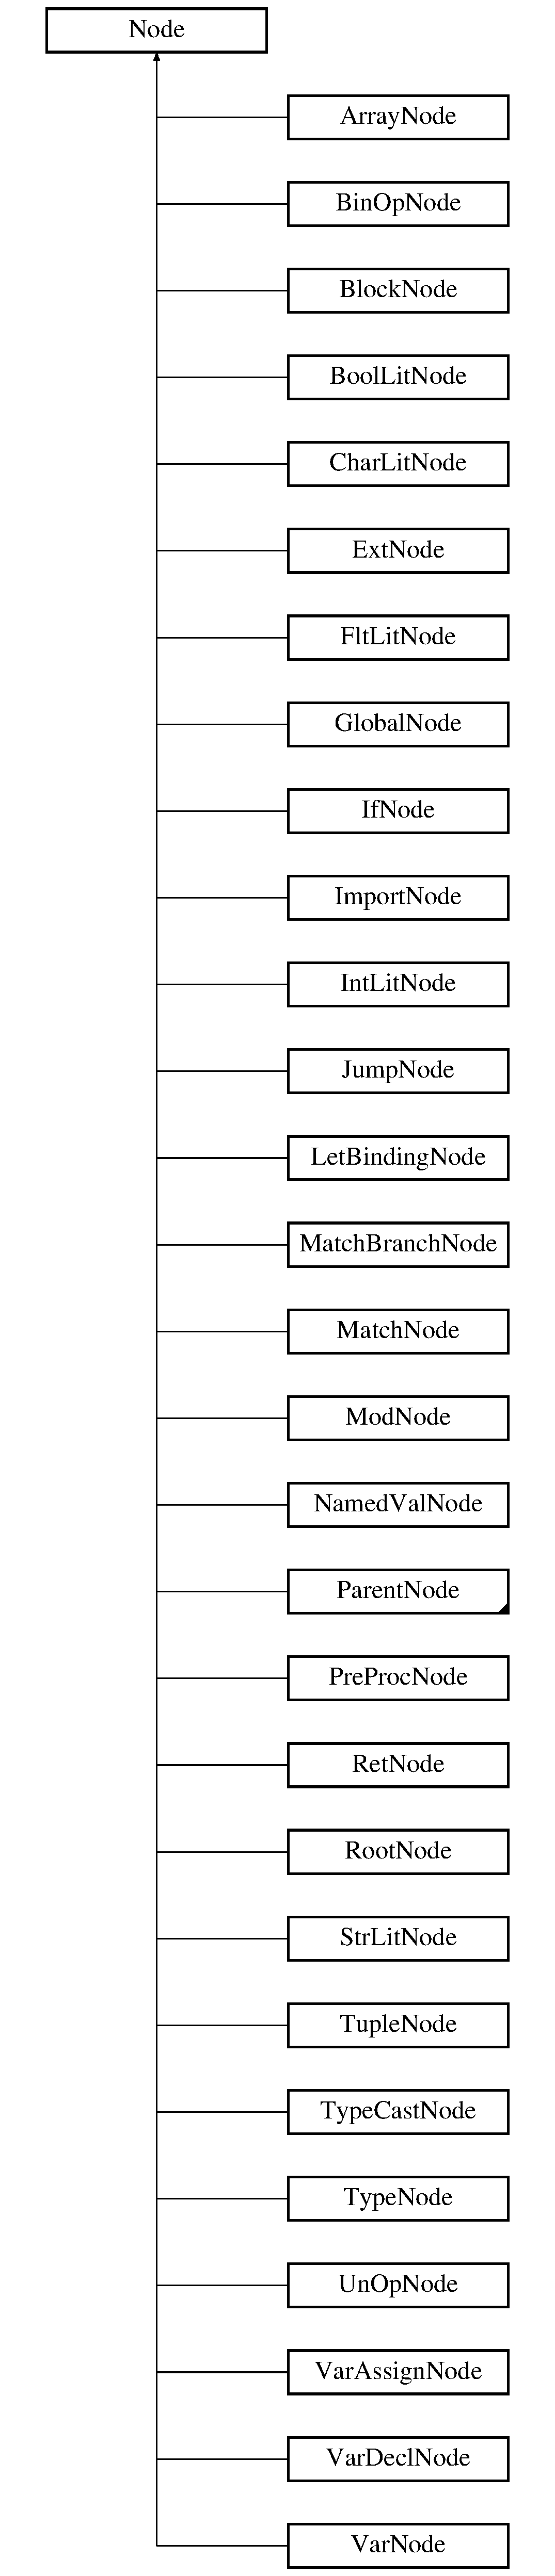
\includegraphics[height=12.000000cm]{structNode}
\end{center}
\end{figure}
\subsection*{Public Member Functions}
\begin{DoxyCompactItemize}
\item 
\mbox{\Hypertarget{structNode_aa4de6ea3d3ed834945f1f19bcd7252b4}\label{structNode_aa4de6ea3d3ed834945f1f19bcd7252b4}} 
virtual void {\bfseries print} (void)=0
\item 
\mbox{\Hypertarget{structNode_ae2a9af0063bebb4530d35f4f44966bfa}\label{structNode_ae2a9af0063bebb4530d35f4f44966bfa}} 
virtual \hyperlink{structTypedValue}{Typed\+Value} $\ast$ {\bfseries compile} (\hyperlink{structante_1_1Compiler}{Compiler} $\ast$)=0
\item 
\mbox{\Hypertarget{structNode_af869c1880640503e7ce8b7f977d2e26e}\label{structNode_af869c1880640503e7ce8b7f977d2e26e}} 
\hyperlink{structNodeIterator}{Node\+Iterator} {\bfseries begin} ()
\item 
\mbox{\Hypertarget{structNode_a74e2abe32a0aab98338e46305533f79f}\label{structNode_a74e2abe32a0aab98338e46305533f79f}} 
\hyperlink{structNodeIterator}{Node\+Iterator} {\bfseries end} ()
\item 
\mbox{\Hypertarget{structNode_af9f9dd5d2937a8f2e411f5244fd4d0dc}\label{structNode_af9f9dd5d2937a8f2e411f5244fd4d0dc}} 
{\bfseries Node} (L\+O\+C\+\_\+\+TY \&l)
\end{DoxyCompactItemize}
\subsection*{Public Attributes}
\begin{DoxyCompactItemize}
\item 
\mbox{\Hypertarget{structNode_a018e5154229ceeaba9f76f42588585fd}\label{structNode_a018e5154229ceeaba9f76f42588585fd}} 
unique\+\_\+ptr$<$ \hyperlink{structNode}{Node} $>$ {\bfseries next}
\item 
\mbox{\Hypertarget{structNode_a632ea91c6a13082308f7692649a68880}\label{structNode_a632ea91c6a13082308f7692649a68880}} 
\hyperlink{structNode}{Node} $\ast$ {\bfseries prev}
\item 
\mbox{\Hypertarget{structNode_a87efd1bb0a94659ad56b0ea36d0de6b1}\label{structNode_a87efd1bb0a94659ad56b0ea36d0de6b1}} 
L\+O\+C\+\_\+\+TY {\bfseries loc}
\end{DoxyCompactItemize}


The documentation for this struct was generated from the following files\+:\begin{DoxyCompactItemize}
\item 
/home/rndmprsn/\+Code/\+Ante/include/parser.\+h\item 
/home/rndmprsn/\+Code/\+Ante/src/ptree.\+cpp\end{DoxyCompactItemize}

\hypertarget{structNodeIterator}{}\section{Node\+Iterator Struct Reference}
\label{structNodeIterator}\index{Node\+Iterator@{Node\+Iterator}}
\subsection*{Public Member Functions}
\begin{DoxyCompactItemize}
\item 
\mbox{\Hypertarget{structNodeIterator_a9241b5682e6021a4d9154629c2dc8a05}\label{structNodeIterator_a9241b5682e6021a4d9154629c2dc8a05}} 
\hyperlink{structNodeIterator}{Node\+Iterator} {\bfseries operator++} ()
\item 
\mbox{\Hypertarget{structNodeIterator_a803b7a02f66621be46044937d4a119c7}\label{structNodeIterator_a803b7a02f66621be46044937d4a119c7}} 
\hyperlink{structNode}{Node} $\ast$ {\bfseries operator$\ast$} ()
\item 
\mbox{\Hypertarget{structNodeIterator_a93cdfc1747402c0106a684ce3f4265ad}\label{structNodeIterator_a93cdfc1747402c0106a684ce3f4265ad}} 
bool {\bfseries operator==} (\hyperlink{structNodeIterator}{Node\+Iterator} r)
\item 
\mbox{\Hypertarget{structNodeIterator_a2c5e8390dddfcdaded7ddced41e45076}\label{structNodeIterator_a2c5e8390dddfcdaded7ddced41e45076}} 
bool {\bfseries operator!=} (\hyperlink{structNodeIterator}{Node\+Iterator} r)
\end{DoxyCompactItemize}
\subsection*{Public Attributes}
\begin{DoxyCompactItemize}
\item 
\mbox{\Hypertarget{structNodeIterator_a3af00d1c6a186001f3b73d475a255540}\label{structNodeIterator_a3af00d1c6a186001f3b73d475a255540}} 
\hyperlink{structNode}{Node} $\ast$ {\bfseries cur}
\end{DoxyCompactItemize}


The documentation for this struct was generated from the following files\+:\begin{DoxyCompactItemize}
\item 
/home/rndmprsn/\+Code/\+Ante/include/parser.\+h\item 
/home/rndmprsn/\+Code/\+Ante/src/ptree.\+cpp\end{DoxyCompactItemize}

\hypertarget{structParentNode}{}\section{Parent\+Node Struct Reference}
\label{structParentNode}\index{Parent\+Node@{Parent\+Node}}
Inheritance diagram for Parent\+Node\+:\begin{figure}[H]
\begin{center}
\leavevmode
\includegraphics[height=3.000000cm]{structParentNode}
\end{center}
\end{figure}
\subsection*{Public Member Functions}
\begin{DoxyCompactItemize}
\item 
\mbox{\Hypertarget{structParentNode_ad963927875f7c5e4bb529a2d4072cffd}\label{structParentNode_ad963927875f7c5e4bb529a2d4072cffd}} 
{\bfseries Parent\+Node} (L\+O\+C\+\_\+\+TY \&loc, \hyperlink{structNode}{Node} $\ast$c)
\end{DoxyCompactItemize}
\subsection*{Public Attributes}
\begin{DoxyCompactItemize}
\item 
\mbox{\Hypertarget{structParentNode_a66b7a4165bc777ba4b0f81117272b4f7}\label{structParentNode_a66b7a4165bc777ba4b0f81117272b4f7}} 
unique\+\_\+ptr$<$ \hyperlink{structNode}{Node} $>$ {\bfseries child}
\end{DoxyCompactItemize}


The documentation for this struct was generated from the following file\+:\begin{DoxyCompactItemize}
\item 
/home/rndmprsn/\+Code/\+Ante/include/parser.\+h\end{DoxyCompactItemize}

\hypertarget{classyy_1_1parser}{}\section{yy\+:\+:parser Class Reference}
\label{classyy_1_1parser}\index{yy\+::parser@{yy\+::parser}}


A Bison parser.  




{\ttfamily \#include $<$yyparser.\+h$>$}

\subsection*{Classes}
\begin{DoxyCompactItemize}
\item 
struct \hyperlink{structyy_1_1parser_1_1basic__symbol}{basic\+\_\+symbol}
\item 
struct \hyperlink{structyy_1_1parser_1_1by__type}{by\+\_\+type}
\begin{DoxyCompactList}\small\item\em Type access provider for token (enum) based symbols. \end{DoxyCompactList}\item 
struct \hyperlink{structyy_1_1parser_1_1syntax__error}{syntax\+\_\+error}
\begin{DoxyCompactList}\small\item\em Syntax errors thrown from user actions. \end{DoxyCompactList}\item 
struct \hyperlink{structyy_1_1parser_1_1token}{token}
\begin{DoxyCompactList}\small\item\em Tokens. \end{DoxyCompactList}\end{DoxyCompactItemize}
\subsection*{Public Types}
\begin{DoxyCompactItemize}
\item 
\mbox{\Hypertarget{classyy_1_1parser_acd86822bc88edf119d2b33d1c08cec7d}\label{classyy_1_1parser_acd86822bc88edf119d2b33d1c08cec7d}} 
enum \{ {\bfseries empty\+\_\+symbol} = -\/2
 \}\begin{DoxyCompactList}\small\item\em The symbol type number to denote an empty symbol. \end{DoxyCompactList}
\item 
\mbox{\Hypertarget{classyy_1_1parser_abb6ca82d9e84da6d4b98e65f650b2456}\label{classyy_1_1parser_abb6ca82d9e84da6d4b98e65f650b2456}} 
typedef int \hyperlink{classyy_1_1parser_abb6ca82d9e84da6d4b98e65f650b2456}{semantic\+\_\+type}
\begin{DoxyCompactList}\small\item\em Symbol semantic values. \end{DoxyCompactList}\item 
\mbox{\Hypertarget{classyy_1_1parser_a6cee0517f5ed9774dd68ee189b62e454}\label{classyy_1_1parser_a6cee0517f5ed9774dd68ee189b62e454}} 
typedef \hyperlink{classyy_1_1location}{location} \hyperlink{classyy_1_1parser_a6cee0517f5ed9774dd68ee189b62e454}{location\+\_\+type}
\begin{DoxyCompactList}\small\item\em Symbol locations. \end{DoxyCompactList}\item 
\mbox{\Hypertarget{classyy_1_1parser_ac1ba3f834abfa251ea746c4ca8da5a85}\label{classyy_1_1parser_ac1ba3f834abfa251ea746c4ca8da5a85}} 
typedef token\+::yytokentype \hyperlink{classyy_1_1parser_ac1ba3f834abfa251ea746c4ca8da5a85}{token\+\_\+type}
\begin{DoxyCompactList}\small\item\em (External) token type, as returned by yylex. \end{DoxyCompactList}\item 
\mbox{\Hypertarget{classyy_1_1parser_a522f5c6c3481d9285b0b991ac12292eb}\label{classyy_1_1parser_a522f5c6c3481d9285b0b991ac12292eb}} 
typedef int \hyperlink{classyy_1_1parser_a522f5c6c3481d9285b0b991ac12292eb}{symbol\+\_\+number\+\_\+type}
\begin{DoxyCompactList}\small\item\em Symbol type\+: an internal symbol number. \end{DoxyCompactList}\item 
\mbox{\Hypertarget{classyy_1_1parser_a9e3963a210d7f2b655d87ca544223ead}\label{classyy_1_1parser_a9e3963a210d7f2b655d87ca544223ead}} 
typedef unsigned char \hyperlink{classyy_1_1parser_a9e3963a210d7f2b655d87ca544223ead}{token\+\_\+number\+\_\+type}
\begin{DoxyCompactList}\small\item\em Internal symbol number for tokens (subsumed by symbol\+\_\+number\+\_\+type). \end{DoxyCompactList}\item 
\mbox{\Hypertarget{classyy_1_1parser_aa8024edbba983aa5cd3e88c3a4dcacc9}\label{classyy_1_1parser_aa8024edbba983aa5cd3e88c3a4dcacc9}} 
typedef \hyperlink{structyy_1_1parser_1_1basic__symbol}{basic\+\_\+symbol}$<$ \hyperlink{structyy_1_1parser_1_1by__type}{by\+\_\+type} $>$ \hyperlink{classyy_1_1parser_aa8024edbba983aa5cd3e88c3a4dcacc9}{symbol\+\_\+type}
\begin{DoxyCompactList}\small\item\em \char`\"{}\+External\char`\"{} symbols\+: returned by the scanner. \end{DoxyCompactList}\end{DoxyCompactItemize}
\subsection*{Public Member Functions}
\begin{DoxyCompactItemize}
\item 
\mbox{\Hypertarget{classyy_1_1parser_a933976dee016ee0623704a75a53551a4}\label{classyy_1_1parser_a933976dee016ee0623704a75a53551a4}} 
\hyperlink{classyy_1_1parser_a933976dee016ee0623704a75a53551a4}{parser} ()
\begin{DoxyCompactList}\small\item\em Build a parser object. \end{DoxyCompactList}\item 
virtual int \hyperlink{classyy_1_1parser_ac54cad6da907397a978922bfe246e6f8}{parse} ()
\item 
virtual void \hyperlink{classyy_1_1parser_a92436afd3e4c5cea48994c7b5c52b7e0}{error} (const \hyperlink{classyy_1_1parser_a6cee0517f5ed9774dd68ee189b62e454}{location\+\_\+type} \&loc, const std\+::string \&msg)
\item 
\mbox{\Hypertarget{classyy_1_1parser_a55d4a04712e5fa9f33baed8f92b3eb05}\label{classyy_1_1parser_a55d4a04712e5fa9f33baed8f92b3eb05}} 
void \hyperlink{classyy_1_1parser_a55d4a04712e5fa9f33baed8f92b3eb05}{error} (const \hyperlink{structyy_1_1parser_1_1syntax__error}{syntax\+\_\+error} \&err)
\begin{DoxyCompactList}\small\item\em Report a syntax error. \end{DoxyCompactList}\end{DoxyCompactItemize}


\subsection{Detailed Description}
A Bison parser. 

\subsection{Member Function Documentation}
\mbox{\Hypertarget{classyy_1_1parser_a92436afd3e4c5cea48994c7b5c52b7e0}\label{classyy_1_1parser_a92436afd3e4c5cea48994c7b5c52b7e0}} 
\index{yy\+::parser@{yy\+::parser}!error@{error}}
\index{error@{error}!yy\+::parser@{yy\+::parser}}
\subsubsection{\texorpdfstring{error()}{error()}}
{\footnotesize\ttfamily virtual void yy\+::parser\+::error (\begin{DoxyParamCaption}\item[{const \hyperlink{classyy_1_1parser_a6cee0517f5ed9774dd68ee189b62e454}{location\+\_\+type} \&}]{loc,  }\item[{const std\+::string \&}]{msg }\end{DoxyParamCaption})\hspace{0.3cm}{\ttfamily [virtual]}}

Report a syntax error. 
\begin{DoxyParams}{Parameters}
{\em loc} & where the syntax error is found. \\
\hline
{\em msg} & a description of the syntax error. \\
\hline
\end{DoxyParams}
\mbox{\Hypertarget{classyy_1_1parser_ac54cad6da907397a978922bfe246e6f8}\label{classyy_1_1parser_ac54cad6da907397a978922bfe246e6f8}} 
\index{yy\+::parser@{yy\+::parser}!parse@{parse}}
\index{parse@{parse}!yy\+::parser@{yy\+::parser}}
\subsubsection{\texorpdfstring{parse()}{parse()}}
{\footnotesize\ttfamily int yy\+::parser\+::parse (\begin{DoxyParamCaption}{ }\end{DoxyParamCaption})\hspace{0.3cm}{\ttfamily [virtual]}}

Parse. \begin{DoxyReturn}{Returns}
0 iff parsing succeeded. 
\end{DoxyReturn}
Length of the R\+HS of the rule being reduced.

The lookahead symbol.

The locations where the error started and ended.

The return value of parse (). 

The documentation for this class was generated from the following files\+:\begin{DoxyCompactItemize}
\item 
/home/rndmprsn/\+Code/\+Ante/include/\hyperlink{yyparser_8h}{yyparser.\+h}\item 
/home/rndmprsn/\+Code/\+Ante/src/parser.\+cpp\end{DoxyCompactItemize}

\hypertarget{classyy_1_1position}{}\section{yy\+:\+:position Class Reference}
\label{classyy_1_1position}\index{yy\+::position@{yy\+::position}}


Abstract a position.  




{\ttfamily \#include $<$position.\+hh$>$}

\subsection*{Public Member Functions}
\begin{DoxyCompactItemize}
\item 
\mbox{\Hypertarget{classyy_1_1position_ad3fcd2dd0259a48f24451f7a2dc620c8}\label{classyy_1_1position_ad3fcd2dd0259a48f24451f7a2dc620c8}} 
\hyperlink{classyy_1_1position_ad3fcd2dd0259a48f24451f7a2dc620c8}{position} (std\+::string $\ast$f=Y\+Y\+\_\+\+N\+U\+L\+L\+P\+TR, unsigned int l=1u, unsigned int c=1u)
\begin{DoxyCompactList}\small\item\em Construct a position. \end{DoxyCompactList}\item 
\mbox{\Hypertarget{classyy_1_1position_ab00c8d19ee14c5ed6a2fc344f4b6e6a1}\label{classyy_1_1position_ab00c8d19ee14c5ed6a2fc344f4b6e6a1}} 
void \hyperlink{classyy_1_1position_ab00c8d19ee14c5ed6a2fc344f4b6e6a1}{initialize} (std\+::string $\ast$fn=Y\+Y\+\_\+\+N\+U\+L\+L\+P\+TR, unsigned int l=1u, unsigned int c=1u)
\begin{DoxyCompactList}\small\item\em Initialization. \end{DoxyCompactList}\end{DoxyCompactItemize}
\begin{Indent}\textbf{ Line and Column related manipulators}\par
\begin{DoxyCompactItemize}
\item 
\mbox{\Hypertarget{classyy_1_1position_a4fbdd03b4e09fa8755d79d3e675d6d3a}\label{classyy_1_1position_a4fbdd03b4e09fa8755d79d3e675d6d3a}} 
void \hyperlink{classyy_1_1position_a4fbdd03b4e09fa8755d79d3e675d6d3a}{lines} (int count=1)
\begin{DoxyCompactList}\small\item\em (line related) Advance to the C\+O\+U\+NT next lines. \end{DoxyCompactList}\item 
\mbox{\Hypertarget{classyy_1_1position_ab15e0388c4fd433aa19c2435e49f72e9}\label{classyy_1_1position_ab15e0388c4fd433aa19c2435e49f72e9}} 
void \hyperlink{classyy_1_1position_ab15e0388c4fd433aa19c2435e49f72e9}{columns} (int count=1)
\begin{DoxyCompactList}\small\item\em (column related) Advance to the C\+O\+U\+NT next columns. \end{DoxyCompactList}\end{DoxyCompactItemize}
\end{Indent}
\subsection*{Public Attributes}
\begin{DoxyCompactItemize}
\item 
\mbox{\Hypertarget{classyy_1_1position_a88d2d070ec4751e5d5b1999bb2dc2116}\label{classyy_1_1position_a88d2d070ec4751e5d5b1999bb2dc2116}} 
std\+::string $\ast$ \hyperlink{classyy_1_1position_a88d2d070ec4751e5d5b1999bb2dc2116}{filename}
\begin{DoxyCompactList}\small\item\em File name to which this position refers. \end{DoxyCompactList}\item 
\mbox{\Hypertarget{classyy_1_1position_aa3806654fd62786a0446a461d55755d6}\label{classyy_1_1position_aa3806654fd62786a0446a461d55755d6}} 
unsigned int \hyperlink{classyy_1_1position_aa3806654fd62786a0446a461d55755d6}{line}
\begin{DoxyCompactList}\small\item\em Current line number. \end{DoxyCompactList}\item 
\mbox{\Hypertarget{classyy_1_1position_ada60c2dbba2e05705265f8359f722c4f}\label{classyy_1_1position_ada60c2dbba2e05705265f8359f722c4f}} 
unsigned int \hyperlink{classyy_1_1position_ada60c2dbba2e05705265f8359f722c4f}{column}
\begin{DoxyCompactList}\small\item\em Current column number. \end{DoxyCompactList}\end{DoxyCompactItemize}


\subsection{Detailed Description}
Abstract a position. 

The documentation for this class was generated from the following file\+:\begin{DoxyCompactItemize}
\item 
/home/rndmprsn/\+Code/\+Ante/include/position.\+hh\end{DoxyCompactItemize}

\hypertarget{structPreProcNode}{}\section{Pre\+Proc\+Node Struct Reference}
\label{structPreProcNode}\index{Pre\+Proc\+Node@{Pre\+Proc\+Node}}
Inheritance diagram for Pre\+Proc\+Node\+:\begin{figure}[H]
\begin{center}
\leavevmode
\includegraphics[height=2.000000cm]{structPreProcNode}
\end{center}
\end{figure}
\subsection*{Public Member Functions}
\begin{DoxyCompactItemize}
\item 
\mbox{\Hypertarget{structPreProcNode_a4d98f4a7ee76a87619559f78610dfafd}\label{structPreProcNode_a4d98f4a7ee76a87619559f78610dfafd}} 
\hyperlink{structTypedValue}{Typed\+Value} $\ast$ {\bfseries compile} (\hyperlink{structante_1_1Compiler}{Compiler} $\ast$)
\item 
\mbox{\Hypertarget{structPreProcNode_ad31437b329fbe48ca2bb2ce4d2588538}\label{structPreProcNode_ad31437b329fbe48ca2bb2ce4d2588538}} 
void {\bfseries print} (void)
\item 
\mbox{\Hypertarget{structPreProcNode_ab8aec3b3836fe8c852987d42d96ccde4}\label{structPreProcNode_ab8aec3b3836fe8c852987d42d96ccde4}} 
{\bfseries Pre\+Proc\+Node} (L\+O\+C\+\_\+\+TY \&loc, \hyperlink{structNode}{Node} $\ast$e)
\end{DoxyCompactItemize}
\subsection*{Public Attributes}
\begin{DoxyCompactItemize}
\item 
\mbox{\Hypertarget{structPreProcNode_a5dde53ee64f5c22c1e553a56bd9bc5a8}\label{structPreProcNode_a5dde53ee64f5c22c1e553a56bd9bc5a8}} 
unique\+\_\+ptr$<$ \hyperlink{structNode}{Node} $>$ {\bfseries expr}
\end{DoxyCompactItemize}


The documentation for this struct was generated from the following files\+:\begin{DoxyCompactItemize}
\item 
/home/rndmprsn/\+Code/\+Ante/include/parser.\+h\item 
/home/rndmprsn/\+Code/\+Ante/src/compiler.\+cpp\item 
/home/rndmprsn/\+Code/\+Ante/src/nodeprinter.\+cpp\end{DoxyCompactItemize}

\hypertarget{structRetNode}{}\section{Ret\+Node Struct Reference}
\label{structRetNode}\index{Ret\+Node@{Ret\+Node}}
Inheritance diagram for Ret\+Node\+:\begin{figure}[H]
\begin{center}
\leavevmode
\includegraphics[height=2.000000cm]{structRetNode}
\end{center}
\end{figure}
\subsection*{Public Member Functions}
\begin{DoxyCompactItemize}
\item 
\mbox{\Hypertarget{structRetNode_acadca5e50e51de4d100afecc35fd1c18}\label{structRetNode_acadca5e50e51de4d100afecc35fd1c18}} 
\hyperlink{structTypedValue}{Typed\+Value} $\ast$ {\bfseries compile} (\hyperlink{structante_1_1Compiler}{Compiler} $\ast$)
\item 
\mbox{\Hypertarget{structRetNode_a15d1f5b8f2793a261162396b68af58bf}\label{structRetNode_a15d1f5b8f2793a261162396b68af58bf}} 
void {\bfseries print} (void)
\item 
\mbox{\Hypertarget{structRetNode_a7dd6b9c547398e9ea18124ac9cbcdc17}\label{structRetNode_a7dd6b9c547398e9ea18124ac9cbcdc17}} 
{\bfseries Ret\+Node} (L\+O\+C\+\_\+\+TY \&loc, \hyperlink{structNode}{Node} $\ast$e)
\end{DoxyCompactItemize}
\subsection*{Public Attributes}
\begin{DoxyCompactItemize}
\item 
\mbox{\Hypertarget{structRetNode_ada00e6cc35027a85d5b8283a5c30799e}\label{structRetNode_ada00e6cc35027a85d5b8283a5c30799e}} 
unique\+\_\+ptr$<$ \hyperlink{structNode}{Node} $>$ {\bfseries expr}
\end{DoxyCompactItemize}


The documentation for this struct was generated from the following files\+:\begin{DoxyCompactItemize}
\item 
/home/rndmprsn/\+Code/\+Ante/include/parser.\+h\item 
/home/rndmprsn/\+Code/\+Ante/src/compiler.\+cpp\item 
/home/rndmprsn/\+Code/\+Ante/src/nodeprinter.\+cpp\end{DoxyCompactItemize}

\hypertarget{structRootNode}{}\section{Root\+Node Struct Reference}
\label{structRootNode}\index{Root\+Node@{Root\+Node}}
Inheritance diagram for Root\+Node\+:\begin{figure}[H]
\begin{center}
\leavevmode
\includegraphics[height=2.000000cm]{structRootNode}
\end{center}
\end{figure}
\subsection*{Public Member Functions}
\begin{DoxyCompactItemize}
\item 
\mbox{\Hypertarget{structRootNode_a9921ffd2752215074bb0ca89c8e00236}\label{structRootNode_a9921ffd2752215074bb0ca89c8e00236}} 
\hyperlink{structTypedValue}{Typed\+Value} $\ast$ {\bfseries compile} (\hyperlink{structante_1_1Compiler}{Compiler} $\ast$)
\item 
\mbox{\Hypertarget{structRootNode_a51164b78e8f7fb2156b9bbe70215493c}\label{structRootNode_a51164b78e8f7fb2156b9bbe70215493c}} 
void {\bfseries print} ()
\item 
\mbox{\Hypertarget{structRootNode_a6b4ca93d6c9509cd047ae12bd1644177}\label{structRootNode_a6b4ca93d6c9509cd047ae12bd1644177}} 
{\bfseries Root\+Node} (L\+O\+C\+\_\+\+TY \&loc)
\end{DoxyCompactItemize}
\subsection*{Public Attributes}
\begin{DoxyCompactItemize}
\item 
\mbox{\Hypertarget{structRootNode_a19febba060ea41f0c58644d57961dec1}\label{structRootNode_a19febba060ea41f0c58644d57961dec1}} 
vector$<$ \hyperlink{structFuncDeclNode}{Func\+Decl\+Node} $\ast$ $>$ {\bfseries funcs}
\item 
\mbox{\Hypertarget{structRootNode_a117ef77726fd5f3c3e4ead6abad58dc9}\label{structRootNode_a117ef77726fd5f3c3e4ead6abad58dc9}} 
vector$<$ \hyperlink{structTraitNode}{Trait\+Node} $\ast$ $>$ {\bfseries traits}
\item 
\mbox{\Hypertarget{structRootNode_aabc83f42e419bcb09678aa661256b3e4}\label{structRootNode_aabc83f42e419bcb09678aa661256b3e4}} 
vector$<$ \hyperlink{structExtNode}{Ext\+Node} $\ast$ $>$ {\bfseries extensions}
\item 
\mbox{\Hypertarget{structRootNode_a4fec05675e4a7ecee8beabfb4801e2aa}\label{structRootNode_a4fec05675e4a7ecee8beabfb4801e2aa}} 
vector$<$ \hyperlink{structDataDeclNode}{Data\+Decl\+Node} $\ast$ $>$ {\bfseries types}
\item 
\mbox{\Hypertarget{structRootNode_ab814cb1540c7ff388c0587f218b984b2}\label{structRootNode_ab814cb1540c7ff388c0587f218b984b2}} 
vector$<$ unique\+\_\+ptr$<$ \hyperlink{structImportNode}{Import\+Node} $>$ $>$ {\bfseries imports}
\item 
\mbox{\Hypertarget{structRootNode_afe384fca3477b96b61f6379733a96902}\label{structRootNode_afe384fca3477b96b61f6379733a96902}} 
vector$<$ unique\+\_\+ptr$<$ \hyperlink{structNode}{Node} $>$ $>$ {\bfseries main}
\end{DoxyCompactItemize}


The documentation for this struct was generated from the following files\+:\begin{DoxyCompactItemize}
\item 
/home/rndmprsn/\+Code/\+Ante/include/parser.\+h\item 
/home/rndmprsn/\+Code/\+Ante/src/compiler.\+cpp\item 
/home/rndmprsn/\+Code/\+Ante/src/nodeprinter.\+cpp\end{DoxyCompactItemize}

\hypertarget{classyy_1_1slice}{}\section{yy\+:\+:slice$<$ T, S $>$ Class Template Reference}
\label{classyy_1_1slice}\index{yy\+::slice$<$ T, S $>$@{yy\+::slice$<$ T, S $>$}}


Present a slice of the top of a stack.  




{\ttfamily \#include $<$stack.\+hh$>$}

\subsection*{Public Member Functions}
\begin{DoxyCompactItemize}
\item 
\mbox{\Hypertarget{classyy_1_1slice_a09b1750a81ae90227fdceb482fa06797}\label{classyy_1_1slice_a09b1750a81ae90227fdceb482fa06797}} 
{\bfseries slice} (const S \&\hyperlink{classyy_1_1stack}{stack}, unsigned int range)
\item 
\mbox{\Hypertarget{classyy_1_1slice_a1b3639b2fffe50544d335fb3f5763c1f}\label{classyy_1_1slice_a1b3639b2fffe50544d335fb3f5763c1f}} 
const T \& {\bfseries operator\mbox{[}$\,$\mbox{]}} (unsigned int i) const
\end{DoxyCompactItemize}


\subsection{Detailed Description}
\subsubsection*{template$<$class T, class S = stack$<$\+T$>$$>$\newline
class yy\+::slice$<$ T, S $>$}

Present a slice of the top of a stack. 

The documentation for this class was generated from the following file\+:\begin{DoxyCompactItemize}
\item 
/home/rndmprsn/\+Code/\+Ante/include/stack.\+hh\end{DoxyCompactItemize}

\hypertarget{classyy_1_1stack}{}\section{yy\+:\+:stack$<$ T, S $>$ Class Template Reference}
\label{classyy_1_1stack}\index{yy\+::stack$<$ T, S $>$@{yy\+::stack$<$ T, S $>$}}
\subsection*{Public Types}
\begin{DoxyCompactItemize}
\item 
\mbox{\Hypertarget{classyy_1_1stack_a959921144f243952520a2178121cbe6f}\label{classyy_1_1stack_a959921144f243952520a2178121cbe6f}} 
typedef S\+::reverse\+\_\+iterator {\bfseries iterator}
\item 
\mbox{\Hypertarget{classyy_1_1stack_a0cab3a74b0947ce6de68c3520b9229ab}\label{classyy_1_1stack_a0cab3a74b0947ce6de68c3520b9229ab}} 
typedef S\+::const\+\_\+reverse\+\_\+iterator {\bfseries const\+\_\+iterator}
\end{DoxyCompactItemize}
\subsection*{Public Member Functions}
\begin{DoxyCompactItemize}
\item 
\mbox{\Hypertarget{classyy_1_1stack_af4277ae80177abc36f242c3646cbcfbe}\label{classyy_1_1stack_af4277ae80177abc36f242c3646cbcfbe}} 
{\bfseries stack} (unsigned int n)
\item 
\mbox{\Hypertarget{classyy_1_1stack_a1058b8b7e1a3e0aa7b1e6f2f1a62c234}\label{classyy_1_1stack_a1058b8b7e1a3e0aa7b1e6f2f1a62c234}} 
T \& {\bfseries operator\mbox{[}$\,$\mbox{]}} (unsigned int i)
\item 
\mbox{\Hypertarget{classyy_1_1stack_a248d8971564c62112266438ae86e53d5}\label{classyy_1_1stack_a248d8971564c62112266438ae86e53d5}} 
const T \& {\bfseries operator\mbox{[}$\,$\mbox{]}} (unsigned int i) const
\item 
void \hyperlink{classyy_1_1stack_acf2b971ffb94c77b56fc0249b55250fa}{push} (T \&t)
\item 
\mbox{\Hypertarget{classyy_1_1stack_a0800c0a796cade80c3ce9a785dc87564}\label{classyy_1_1stack_a0800c0a796cade80c3ce9a785dc87564}} 
void {\bfseries pop} (unsigned int n=1)
\item 
\mbox{\Hypertarget{classyy_1_1stack_ae8b2c8309dcdef98210205b1c96b2238}\label{classyy_1_1stack_ae8b2c8309dcdef98210205b1c96b2238}} 
void {\bfseries clear} ()
\item 
\mbox{\Hypertarget{classyy_1_1stack_adff918ad84f227bd3d51eb8ef5c1dc95}\label{classyy_1_1stack_adff918ad84f227bd3d51eb8ef5c1dc95}} 
S\+::size\+\_\+type {\bfseries size} () const
\item 
\mbox{\Hypertarget{classyy_1_1stack_ab7f28676a74b21114422d94d10b971a7}\label{classyy_1_1stack_ab7f28676a74b21114422d94d10b971a7}} 
const\+\_\+iterator {\bfseries begin} () const
\item 
\mbox{\Hypertarget{classyy_1_1stack_a7d5b4e82ede55ba095de45da26600a8c}\label{classyy_1_1stack_a7d5b4e82ede55ba095de45da26600a8c}} 
const\+\_\+iterator {\bfseries end} () const
\end{DoxyCompactItemize}


\subsection{Member Function Documentation}
\mbox{\Hypertarget{classyy_1_1stack_acf2b971ffb94c77b56fc0249b55250fa}\label{classyy_1_1stack_acf2b971ffb94c77b56fc0249b55250fa}} 
\index{yy\+::stack@{yy\+::stack}!push@{push}}
\index{push@{push}!yy\+::stack@{yy\+::stack}}
\subsubsection{\texorpdfstring{push()}{push()}}
{\footnotesize\ttfamily template$<$class T, class S = std\+::vector$<$\+T$>$$>$ \\
void \hyperlink{classyy_1_1stack}{yy\+::stack}$<$ T, S $>$\+::push (\begin{DoxyParamCaption}\item[{T \&}]{t }\end{DoxyParamCaption})\hspace{0.3cm}{\ttfamily [inline]}}

Steal the contents of {\itshape t}.

Close to move-\/semantics. 

The documentation for this class was generated from the following file\+:\begin{DoxyCompactItemize}
\item 
/home/rndmprsn/\+Code/\+Ante/include/stack.\+hh\end{DoxyCompactItemize}

\hypertarget{structStrLitNode}{}\section{Str\+Lit\+Node Struct Reference}
\label{structStrLitNode}\index{Str\+Lit\+Node@{Str\+Lit\+Node}}
Inheritance diagram for Str\+Lit\+Node\+:\begin{figure}[H]
\begin{center}
\leavevmode
\includegraphics[height=2.000000cm]{structStrLitNode}
\end{center}
\end{figure}
\subsection*{Public Member Functions}
\begin{DoxyCompactItemize}
\item 
\mbox{\Hypertarget{structStrLitNode_ab80f0394ea38907501f228682dd410dc}\label{structStrLitNode_ab80f0394ea38907501f228682dd410dc}} 
\hyperlink{structTypedValue}{Typed\+Value} $\ast$ {\bfseries compile} (\hyperlink{structante_1_1Compiler}{Compiler} $\ast$)
\item 
\mbox{\Hypertarget{structStrLitNode_aa82d55c93bc0cdf4d908122f2968c46e}\label{structStrLitNode_aa82d55c93bc0cdf4d908122f2968c46e}} 
void {\bfseries print} (void)
\item 
\mbox{\Hypertarget{structStrLitNode_a93362d423a43bfb2beac557bf130075c}\label{structStrLitNode_a93362d423a43bfb2beac557bf130075c}} 
{\bfseries Str\+Lit\+Node} (L\+O\+C\+\_\+\+TY \&loc, string s)
\end{DoxyCompactItemize}
\subsection*{Public Attributes}
\begin{DoxyCompactItemize}
\item 
\mbox{\Hypertarget{structStrLitNode_a3b893d87683075809d5c877b19df1507}\label{structStrLitNode_a3b893d87683075809d5c877b19df1507}} 
string {\bfseries val}
\end{DoxyCompactItemize}


The documentation for this struct was generated from the following files\+:\begin{DoxyCompactItemize}
\item 
/home/rndmprsn/\+Code/\+Ante/include/parser.\+h\item 
/home/rndmprsn/\+Code/\+Ante/src/compiler.\+cpp\item 
/home/rndmprsn/\+Code/\+Ante/src/nodeprinter.\+cpp\end{DoxyCompactItemize}

\hypertarget{structyy_1_1parser_1_1syntax__error}{}\section{yy\+:\+:parser\+:\+:syntax\+\_\+error Struct Reference}
\label{structyy_1_1parser_1_1syntax__error}\index{yy\+::parser\+::syntax\+\_\+error@{yy\+::parser\+::syntax\+\_\+error}}


Syntax errors thrown from user actions.  




{\ttfamily \#include $<$yyparser.\+h$>$}

Inheritance diagram for yy\+:\+:parser\+:\+:syntax\+\_\+error\+:\begin{figure}[H]
\begin{center}
\leavevmode
\includegraphics[height=2.000000cm]{structyy_1_1parser_1_1syntax__error}
\end{center}
\end{figure}
\subsection*{Public Member Functions}
\begin{DoxyCompactItemize}
\item 
\mbox{\Hypertarget{structyy_1_1parser_1_1syntax__error_aa40bb3085ae32f3ec5a42e2a01736cd4}\label{structyy_1_1parser_1_1syntax__error_aa40bb3085ae32f3ec5a42e2a01736cd4}} 
{\bfseries syntax\+\_\+error} (const \hyperlink{classyy_1_1parser_a6cee0517f5ed9774dd68ee189b62e454}{location\+\_\+type} \&l, const std\+::string \&m)
\end{DoxyCompactItemize}
\subsection*{Public Attributes}
\begin{DoxyCompactItemize}
\item 
\mbox{\Hypertarget{structyy_1_1parser_1_1syntax__error_a18f10cd4bd4c27a2fba391a67fef856a}\label{structyy_1_1parser_1_1syntax__error_a18f10cd4bd4c27a2fba391a67fef856a}} 
\hyperlink{classyy_1_1parser_a6cee0517f5ed9774dd68ee189b62e454}{location\+\_\+type} {\bfseries location}
\end{DoxyCompactItemize}


\subsection{Detailed Description}
Syntax errors thrown from user actions. 

The documentation for this struct was generated from the following files\+:\begin{DoxyCompactItemize}
\item 
/home/rndmprsn/\+Code/\+Ante/include/\hyperlink{yyparser_8h}{yyparser.\+h}\item 
/home/rndmprsn/\+Code/\+Ante/src/parser.\+cpp\end{DoxyCompactItemize}

\hypertarget{structyy_1_1parser_1_1token}{}\section{yy\+:\+:parser\+:\+:token Struct Reference}
\label{structyy_1_1parser_1_1token}\index{yy\+::parser\+::token@{yy\+::parser\+::token}}


Tokens.  




{\ttfamily \#include $<$yyparser.\+h$>$}

\subsection*{Public Types}
\begin{DoxyCompactItemize}
\item 
\mbox{\Hypertarget{structyy_1_1parser_1_1token_a90b63e7f9dd7177dd3bf01c58c408475}\label{structyy_1_1parser_1_1token_a90b63e7f9dd7177dd3bf01c58c408475}} 
enum {\bfseries yytokentype} \{ \newline
{\bfseries Ident} = 258, 
{\bfseries User\+Type} = 259, 
{\bfseries Type\+Var} = 260, 
{\bfseries I8} = 261, 
\newline
{\bfseries I16} = 262, 
{\bfseries I32} = 263, 
{\bfseries I64} = 264, 
{\bfseries U8} = 265, 
\newline
{\bfseries U16} = 266, 
{\bfseries U32} = 267, 
{\bfseries U64} = 268, 
{\bfseries Isz} = 269, 
\newline
{\bfseries Usz} = 270, 
{\bfseries F16} = 271, 
{\bfseries F32} = 272, 
{\bfseries F64} = 273, 
\newline
{\bfseries C8} = 274, 
{\bfseries C32} = 275, 
{\bfseries Bool} = 276, 
{\bfseries Void} = 277, 
\newline
{\bfseries Eq} = 278, 
{\bfseries Not\+Eq} = 279, 
{\bfseries Add\+Eq} = 280, 
{\bfseries Sub\+Eq} = 281, 
\newline
{\bfseries Mul\+Eq} = 282, 
{\bfseries Div\+Eq} = 283, 
{\bfseries Grtr\+Eq} = 284, 
{\bfseries Lesr\+Eq} = 285, 
\newline
{\bfseries Or} = 286, 
{\bfseries And} = 287, 
{\bfseries Range} = 288, 
{\bfseries R\+Arrow} = 289, 
\newline
{\bfseries ApplyL} = 290, 
{\bfseries ApplyR} = 291, 
{\bfseries Append} = 292, 
{\bfseries New} = 293, 
\newline
{\bfseries Not} = 294, 
{\bfseries True} = 295, 
{\bfseries False} = 296, 
{\bfseries Int\+Lit} = 297, 
\newline
{\bfseries Flt\+Lit} = 298, 
{\bfseries Str\+Lit} = 299, 
{\bfseries Char\+Lit} = 300, 
{\bfseries Return} = 301, 
\newline
{\bfseries If} = 302, 
{\bfseries Then} = 303, 
{\bfseries Elif} = 304, 
{\bfseries Else} = 305, 
\newline
{\bfseries For} = 306, 
{\bfseries While} = 307, 
{\bfseries Do} = 308, 
{\bfseries In} = 309, 
\newline
{\bfseries Continue} = 310, 
{\bfseries Break} = 311, 
{\bfseries Import} = 312, 
{\bfseries Let} = 313, 
\newline
{\bfseries Var} = 314, 
{\bfseries Match} = 315, 
{\bfseries With} = 316, 
{\bfseries Type} = 317, 
\newline
{\bfseries Trait} = 318, 
{\bfseries Fun} = 319, 
{\bfseries Ext} = 320, 
{\bfseries Pub} = 321, 
\newline
{\bfseries Pri} = 322, 
{\bfseries Pro} = 323, 
{\bfseries Raw} = 324, 
{\bfseries Const} = 325, 
\newline
{\bfseries Noinit} = 326, 
{\bfseries Mut} = 327, 
{\bfseries Global} = 328, 
{\bfseries Where} = 329, 
\newline
{\bfseries Newline} = 330, 
{\bfseries Indent} = 331, 
{\bfseries Unindent} = 332, 
{\bfseries L\+OW} = 333, 
\newline
{\bfseries M\+E\+D\+L\+OW} = 334, 
{\bfseries S\+T\+MT} = 335, 
{\bfseries E\+N\+D\+IF} = 336, 
{\bfseries M\+E\+D\+IF} = 337, 
\newline
{\bfseries M\+ED} = 338, 
{\bfseries M\+O\+D\+I\+F\+I\+ER} = 339, 
{\bfseries T\+Y\+PE} = 340, 
{\bfseries F\+U\+NC} = 341, 
\newline
{\bfseries L\+I\+T\+E\+R\+A\+LS} = 342, 
{\bfseries H\+I\+GH} = 343
 \}
\end{DoxyCompactItemize}


\subsection{Detailed Description}
Tokens. 

The documentation for this struct was generated from the following file\+:\begin{DoxyCompactItemize}
\item 
/home/rndmprsn/\+Code/\+Ante/include/\hyperlink{yyparser_8h}{yyparser.\+h}\end{DoxyCompactItemize}

\hypertarget{structTrait}{}\section{Trait Struct Reference}
\label{structTrait}\index{Trait@{Trait}}
\subsection*{Public Attributes}
\begin{DoxyCompactItemize}
\item 
\mbox{\Hypertarget{structTrait_ab59bc73cb96cac338431039baff7673f}\label{structTrait_ab59bc73cb96cac338431039baff7673f}} 
string {\bfseries name}
\item 
\mbox{\Hypertarget{structTrait_ada8cbf37cb33497fc160c02b7e5be787}\label{structTrait_ada8cbf37cb33497fc160c02b7e5be787}} 
vector$<$ shared\+\_\+ptr$<$ \hyperlink{structFuncDecl}{Func\+Decl} $>$ $>$ {\bfseries funcs}
\end{DoxyCompactItemize}


The documentation for this struct was generated from the following file\+:\begin{DoxyCompactItemize}
\item 
/home/rndmprsn/\+Code/\+Ante/include/compiler.\+h\end{DoxyCompactItemize}

\hypertarget{structTraitNode}{}\section{Trait\+Node Struct Reference}
\label{structTraitNode}\index{Trait\+Node@{Trait\+Node}}
Inheritance diagram for Trait\+Node\+:\begin{figure}[H]
\begin{center}
\leavevmode
\includegraphics[height=3.000000cm]{structTraitNode}
\end{center}
\end{figure}
\subsection*{Public Member Functions}
\begin{DoxyCompactItemize}
\item 
\mbox{\Hypertarget{structTraitNode_afa71e33c1ad788daa2c80f2183c46d9c}\label{structTraitNode_afa71e33c1ad788daa2c80f2183c46d9c}} 
\hyperlink{structTypedValue}{Typed\+Value} $\ast$ {\bfseries compile} (\hyperlink{structante_1_1Compiler}{Compiler} $\ast$)
\item 
\mbox{\Hypertarget{structTraitNode_a02346fd07c8b8958fa8620e5b64dc4be}\label{structTraitNode_a02346fd07c8b8958fa8620e5b64dc4be}} 
void {\bfseries print} (void)
\item 
\mbox{\Hypertarget{structTraitNode_aeadb33930fe6758658f8b74cef96277f}\label{structTraitNode_aeadb33930fe6758658f8b74cef96277f}} 
{\bfseries Trait\+Node} (L\+O\+C\+\_\+\+TY \&loc, string s, \hyperlink{structNode}{Node} $\ast$b)
\end{DoxyCompactItemize}
\subsection*{Public Attributes}
\begin{DoxyCompactItemize}
\item 
\mbox{\Hypertarget{structTraitNode_a461db5dba441516fc36a27cc70a88340}\label{structTraitNode_a461db5dba441516fc36a27cc70a88340}} 
string {\bfseries name}
\end{DoxyCompactItemize}


The documentation for this struct was generated from the following files\+:\begin{DoxyCompactItemize}
\item 
/home/rndmprsn/\+Code/\+Ante/include/parser.\+h\item 
/home/rndmprsn/\+Code/\+Ante/src/compiler.\+cpp\item 
/home/rndmprsn/\+Code/\+Ante/src/nodeprinter.\+cpp\end{DoxyCompactItemize}

\hypertarget{structTupleNode}{}\section{Tuple\+Node Struct Reference}
\label{structTupleNode}\index{Tuple\+Node@{Tuple\+Node}}
Inheritance diagram for Tuple\+Node\+:\begin{figure}[H]
\begin{center}
\leavevmode
\includegraphics[height=2.000000cm]{structTupleNode}
\end{center}
\end{figure}
\subsection*{Public Member Functions}
\begin{DoxyCompactItemize}
\item 
\mbox{\Hypertarget{structTupleNode_afa372a3344d643444b1eda3124cf147f}\label{structTupleNode_afa372a3344d643444b1eda3124cf147f}} 
\hyperlink{structTypedValue}{Typed\+Value} $\ast$ {\bfseries compile} (\hyperlink{structante_1_1Compiler}{Compiler} $\ast$)
\item 
\mbox{\Hypertarget{structTupleNode_abee54ea2edd6d6bf458cd11a42f846ff}\label{structTupleNode_abee54ea2edd6d6bf458cd11a42f846ff}} 
vector$<$ \hyperlink{structTypedValue}{Typed\+Value} $\ast$ $>$ {\bfseries unpack} (\hyperlink{structante_1_1Compiler}{Compiler} $\ast$)
\item 
\mbox{\Hypertarget{structTupleNode_afa2ba0f92f06e6dd9f69af5578961c2e}\label{structTupleNode_afa2ba0f92f06e6dd9f69af5578961c2e}} 
void {\bfseries print} (void)
\item 
\mbox{\Hypertarget{structTupleNode_a3a5dd0e5ff47daa6b0cfcb44d5226616}\label{structTupleNode_a3a5dd0e5ff47daa6b0cfcb44d5226616}} 
{\bfseries Tuple\+Node} (L\+O\+C\+\_\+\+TY \&loc, vector$<$ unique\+\_\+ptr$<$ \hyperlink{structNode}{Node} $>$$>$ \&e)
\end{DoxyCompactItemize}
\subsection*{Public Attributes}
\begin{DoxyCompactItemize}
\item 
\mbox{\Hypertarget{structTupleNode_a2c28da20640de4e5cf615257672e5cee}\label{structTupleNode_a2c28da20640de4e5cf615257672e5cee}} 
vector$<$ unique\+\_\+ptr$<$ \hyperlink{structNode}{Node} $>$ $>$ {\bfseries exprs}
\end{DoxyCompactItemize}


The documentation for this struct was generated from the following files\+:\begin{DoxyCompactItemize}
\item 
/home/rndmprsn/\+Code/\+Ante/include/parser.\+h\item 
/home/rndmprsn/\+Code/\+Ante/src/compiler.\+cpp\item 
/home/rndmprsn/\+Code/\+Ante/src/nodeprinter.\+cpp\end{DoxyCompactItemize}

\hypertarget{structTypeCastNode}{}\section{Type\+Cast\+Node Struct Reference}
\label{structTypeCastNode}\index{Type\+Cast\+Node@{Type\+Cast\+Node}}
Inheritance diagram for Type\+Cast\+Node\+:\begin{figure}[H]
\begin{center}
\leavevmode
\includegraphics[height=2.000000cm]{structTypeCastNode}
\end{center}
\end{figure}
\subsection*{Public Member Functions}
\begin{DoxyCompactItemize}
\item 
\mbox{\Hypertarget{structTypeCastNode_abbca164252a01742e49a6f5c5f01986d}\label{structTypeCastNode_abbca164252a01742e49a6f5c5f01986d}} 
\hyperlink{structTypedValue}{Typed\+Value} $\ast$ {\bfseries compile} (\hyperlink{structante_1_1Compiler}{Compiler} $\ast$)
\item 
\mbox{\Hypertarget{structTypeCastNode_a3bcf4918d611f6c22ee3c7c9f008edc5}\label{structTypeCastNode_a3bcf4918d611f6c22ee3c7c9f008edc5}} 
void {\bfseries print} (void)
\item 
\mbox{\Hypertarget{structTypeCastNode_ac5d766461431f4bc318e6a6b694e194c}\label{structTypeCastNode_ac5d766461431f4bc318e6a6b694e194c}} 
{\bfseries Type\+Cast\+Node} (L\+O\+C\+\_\+\+TY \&loc, \hyperlink{structTypeNode}{Type\+Node} $\ast$ty, \hyperlink{structNode}{Node} $\ast$rv)
\end{DoxyCompactItemize}
\subsection*{Public Attributes}
\begin{DoxyCompactItemize}
\item 
\mbox{\Hypertarget{structTypeCastNode_a565392d66f6c5962699f794f6aada817}\label{structTypeCastNode_a565392d66f6c5962699f794f6aada817}} 
unique\+\_\+ptr$<$ \hyperlink{structTypeNode}{Type\+Node} $>$ {\bfseries type\+Expr}
\item 
\mbox{\Hypertarget{structTypeCastNode_af4420ccf63d9311f3be4e1b47f9a6005}\label{structTypeCastNode_af4420ccf63d9311f3be4e1b47f9a6005}} 
unique\+\_\+ptr$<$ \hyperlink{structNode}{Node} $>$ {\bfseries rval}
\end{DoxyCompactItemize}


The documentation for this struct was generated from the following files\+:\begin{DoxyCompactItemize}
\item 
/home/rndmprsn/\+Code/\+Ante/include/parser.\+h\item 
/home/rndmprsn/\+Code/\+Ante/src/nodeprinter.\+cpp\item 
/home/rndmprsn/\+Code/\+Ante/src/operator.\+cpp\end{DoxyCompactItemize}

\hypertarget{structTypeCheckResult}{}\section{Type\+Check\+Result Struct Reference}
\label{structTypeCheckResult}\index{Type\+Check\+Result@{Type\+Check\+Result}}
\subsection*{Public Types}
\begin{DoxyCompactItemize}
\item 
\mbox{\Hypertarget{structTypeCheckResult_a6e4b97b4233f002c05e2a773bcefee8b}\label{structTypeCheckResult_a6e4b97b4233f002c05e2a773bcefee8b}} 
enum {\bfseries Result} \{ {\bfseries Failure}, 
{\bfseries Success}, 
{\bfseries Success\+With\+Type\+Vars}
 \}
\end{DoxyCompactItemize}
\subsection*{Public Member Functions}
\begin{DoxyCompactItemize}
\item 
\mbox{\Hypertarget{structTypeCheckResult_a0e555444a132e5a79ec8535bc7192893}\label{structTypeCheckResult_a0e555444a132e5a79ec8535bc7192893}} 
\hyperlink{structTypeCheckResult}{Type\+Check\+Result} $\ast$ {\bfseries set\+Res} (bool b)
\item 
\mbox{\Hypertarget{structTypeCheckResult_a447e6b6d1071b6eac981587db960e162}\label{structTypeCheckResult_a447e6b6d1071b6eac981587db960e162}} 
\hyperlink{structTypeCheckResult}{Type\+Check\+Result} $\ast$ {\bfseries set\+Res} (Result r)
\item 
\mbox{\Hypertarget{structTypeCheckResult_a5d4e3cb1e9dbdb57ca07af42ab8e2b65}\label{structTypeCheckResult_a5d4e3cb1e9dbdb57ca07af42ab8e2b65}} 
\hyperlink{structTypeCheckResult}{Type\+Check\+Result} $\ast$ {\bfseries set\+Success} ()
\item 
\mbox{\Hypertarget{structTypeCheckResult_ab66cd36034f7bf24156fc65729850de1}\label{structTypeCheckResult_ab66cd36034f7bf24156fc65729850de1}} 
\hyperlink{structTypeCheckResult}{Type\+Check\+Result} $\ast$ {\bfseries set\+Success\+With\+Type\+Vars} ()
\item 
\mbox{\Hypertarget{structTypeCheckResult_a9ec37d368ac79f1d0da032f8d39911ae}\label{structTypeCheckResult_a9ec37d368ac79f1d0da032f8d39911ae}} 
\hyperlink{structTypeCheckResult}{Type\+Check\+Result} $\ast$ {\bfseries set\+Failure} ()
\item 
\mbox{\Hypertarget{structTypeCheckResult_acc9788ce17024aa37674a8080bc08231}\label{structTypeCheckResult_acc9788ce17024aa37674a8080bc08231}} 
bool {\bfseries operator!} ()
\item 
\mbox{\Hypertarget{structTypeCheckResult_a125ba7fbba05f80d14954eea886abd21}\label{structTypeCheckResult_a125ba7fbba05f80d14954eea886abd21}} 
\hyperlink{structTypeNode}{Type\+Node} $\ast$ {\bfseries get\+Binding\+For} (const string \&s)
\item 
\mbox{\Hypertarget{structTypeCheckResult_a471209ffb1e1fb3584c5883411632f1d}\label{structTypeCheckResult_a471209ffb1e1fb3584c5883411632f1d}} 
{\bfseries Type\+Check\+Result} (Result r)
\item 
\mbox{\Hypertarget{structTypeCheckResult_a0b0a0bd72383ab9e6a20c1e4c9709919}\label{structTypeCheckResult_a0b0a0bd72383ab9e6a20c1e4c9709919}} 
{\bfseries Type\+Check\+Result} (bool r)
\end{DoxyCompactItemize}
\subsection*{Public Attributes}
\begin{DoxyCompactItemize}
\item 
\mbox{\Hypertarget{structTypeCheckResult_ab2e78473529f9ce8f70bc0faae4e2b6c}\label{structTypeCheckResult_ab2e78473529f9ce8f70bc0faae4e2b6c}} 
Result {\bfseries res}
\item 
\mbox{\Hypertarget{structTypeCheckResult_a3983f128bd275f5aa169bba558fae6b0}\label{structTypeCheckResult_a3983f128bd275f5aa169bba558fae6b0}} 
vector$<$ pair$<$ string, unique\+\_\+ptr$<$ \hyperlink{structTypeNode}{Type\+Node} $>$ $>$ $>$ {\bfseries bindings}
\end{DoxyCompactItemize}


The documentation for this struct was generated from the following files\+:\begin{DoxyCompactItemize}
\item 
/home/rndmprsn/\+Code/\+Ante/include/compiler.\+h\item 
/home/rndmprsn/\+Code/\+Ante/src/types.\+cpp\end{DoxyCompactItemize}

\hypertarget{structTypedValue}{}\section{Typed\+Value Struct Reference}
\label{structTypedValue}\index{Typed\+Value@{Typed\+Value}}
Inheritance diagram for Typed\+Value\+:\begin{figure}[H]
\begin{center}
\leavevmode
\includegraphics[height=2.000000cm]{structTypedValue}
\end{center}
\end{figure}
\subsection*{Public Member Functions}
\begin{DoxyCompactItemize}
\item 
\mbox{\Hypertarget{structTypedValue_a6d4b500bb41a72d38da6ae2d35b65f96}\label{structTypedValue_a6d4b500bb41a72d38da6ae2d35b65f96}} 
{\bfseries Typed\+Value} (Value $\ast$v, \hyperlink{structTypeNode}{Type\+Node} $\ast$ty)
\item 
\mbox{\Hypertarget{structTypedValue_a51d0a91961b7f011c4f1eb017a784358}\label{structTypedValue_a51d0a91961b7f011c4f1eb017a784358}} 
{\bfseries Typed\+Value} (Value $\ast$v, unique\+\_\+ptr$<$ \hyperlink{structTypeNode}{Type\+Node} $>$ \&ty)
\item 
\mbox{\Hypertarget{structTypedValue_a1963855af324d427335d40bb8c7de8d6}\label{structTypedValue_a1963855af324d427335d40bb8c7de8d6}} 
Type $\ast$ {\bfseries get\+Type} () const
\item 
\mbox{\Hypertarget{structTypedValue_af8d6267b024979a922dc0e923035c46d}\label{structTypedValue_af8d6267b024979a922dc0e923035c46d}} 
bool {\bfseries has\+Modifier} (int m) const
\item 
\mbox{\Hypertarget{structTypedValue_a8d29edd52c3548609d3705b4bbb70e5e}\label{structTypedValue_a8d29edd52c3548609d3705b4bbb70e5e}} 
void {\bfseries dump} () const
\end{DoxyCompactItemize}
\subsection*{Public Attributes}
\begin{DoxyCompactItemize}
\item 
\mbox{\Hypertarget{structTypedValue_a000a69ab8159d48d891acdb87d286919}\label{structTypedValue_a000a69ab8159d48d891acdb87d286919}} 
Value $\ast$ {\bfseries val}
\item 
\mbox{\Hypertarget{structTypedValue_ae9750aee2108093267d7b1c625deecbb}\label{structTypedValue_ae9750aee2108093267d7b1c625deecbb}} 
unique\+\_\+ptr$<$ \hyperlink{structTypeNode}{Type\+Node} $>$ {\bfseries type}
\end{DoxyCompactItemize}


The documentation for this struct was generated from the following files\+:\begin{DoxyCompactItemize}
\item 
/home/rndmprsn/\+Code/\+Ante/include/compiler.\+h\item 
/home/rndmprsn/\+Code/\+Ante/src/compiler.\+cpp\end{DoxyCompactItemize}

\hypertarget{structTypeNode}{}\section{Type\+Node Struct Reference}
\label{structTypeNode}\index{Type\+Node@{Type\+Node}}
Inheritance diagram for Type\+Node\+:\begin{figure}[H]
\begin{center}
\leavevmode
\includegraphics[height=2.000000cm]{structTypeNode}
\end{center}
\end{figure}
\subsection*{Public Member Functions}
\begin{DoxyCompactItemize}
\item 
\mbox{\Hypertarget{structTypeNode_abcc7d31031ba5aa91ad2447106d18fe1}\label{structTypeNode_abcc7d31031ba5aa91ad2447106d18fe1}} 
unsigned int {\bfseries get\+Size\+In\+Bits} (\hyperlink{structante_1_1Compiler}{Compiler} $\ast$, string $\ast$tn=0)
\item 
\mbox{\Hypertarget{structTypeNode_a76f508e7ee782d4b6df33cd1a4dc47ff}\label{structTypeNode_a76f508e7ee782d4b6df33cd1a4dc47ff}} 
\hyperlink{structTypedValue}{Typed\+Value} $\ast$ {\bfseries compile} (\hyperlink{structante_1_1Compiler}{Compiler} $\ast$)
\item 
\mbox{\Hypertarget{structTypeNode_a337971d5c4deda16361a8ead384713df}\label{structTypeNode_a337971d5c4deda16361a8ead384713df}} 
void {\bfseries print} (void)
\item 
\mbox{\Hypertarget{structTypeNode_a3b502912f8aa88a8b813c35b6a7ea080}\label{structTypeNode_a3b502912f8aa88a8b813c35b6a7ea080}} 
\hyperlink{structTypeNode}{Type\+Node} $\ast$ {\bfseries add\+Modifiers} (\hyperlink{structModNode}{Mod\+Node} $\ast$m)
\item 
\mbox{\Hypertarget{structTypeNode_aa4dbea17d7a305d96480fb96f1881b2b}\label{structTypeNode_aa4dbea17d7a305d96480fb96f1881b2b}} 
\hyperlink{structTypeNode}{Type\+Node} $\ast$ {\bfseries add\+Modifier} (int m)
\item 
\mbox{\Hypertarget{structTypeNode_a87096f107fb3a11b33550d440022709e}\label{structTypeNode_a87096f107fb3a11b33550d440022709e}} 
void {\bfseries copy\+Modifiers\+From} (const \hyperlink{structTypeNode}{Type\+Node} $\ast$tn)
\item 
\mbox{\Hypertarget{structTypeNode_af3bc1ea7c51b54e163c975cc03565f81}\label{structTypeNode_af3bc1ea7c51b54e163c975cc03565f81}} 
bool {\bfseries has\+Modifier} (int m) const
\item 
\mbox{\Hypertarget{structTypeNode_a155b3715b7db5b4a2ef5f4b3fac4819e}\label{structTypeNode_a155b3715b7db5b4a2ef5f4b3fac4819e}} 
{\bfseries Type\+Node} (L\+O\+C\+\_\+\+TY \&loc, Type\+Tag ty, string t\+Name, \hyperlink{structTypeNode}{Type\+Node} $\ast$e\+Ty)
\end{DoxyCompactItemize}
\subsection*{Public Attributes}
\begin{DoxyCompactItemize}
\item 
\mbox{\Hypertarget{structTypeNode_a63723cb9aebf870f328c360aa015bb32}\label{structTypeNode_a63723cb9aebf870f328c360aa015bb32}} 
Type\+Tag {\bfseries type}
\item 
\mbox{\Hypertarget{structTypeNode_a5aadfc959bd39a49a470ac01c7770486}\label{structTypeNode_a5aadfc959bd39a49a470ac01c7770486}} 
string {\bfseries type\+Name}
\item 
\mbox{\Hypertarget{structTypeNode_a79372c9b9f5f2d95591b763a27f13379}\label{structTypeNode_a79372c9b9f5f2d95591b763a27f13379}} 
unique\+\_\+ptr$<$ \hyperlink{structTypeNode}{Type\+Node} $>$ {\bfseries ext\+Ty}
\item 
\mbox{\Hypertarget{structTypeNode_ad59d8bdd4e281ca0d42473fb005d371d}\label{structTypeNode_ad59d8bdd4e281ca0d42473fb005d371d}} 
vector$<$ unique\+\_\+ptr$<$ \hyperlink{structTypeNode}{Type\+Node} $>$ $>$ {\bfseries params}
\item 
\mbox{\Hypertarget{structTypeNode_adbb221a51767aa2c655ee89a6700d01d}\label{structTypeNode_adbb221a51767aa2c655ee89a6700d01d}} 
vector$<$ int $>$ {\bfseries modifiers}
\end{DoxyCompactItemize}


The documentation for this struct was generated from the following files\+:\begin{DoxyCompactItemize}
\item 
/home/rndmprsn/\+Code/\+Ante/include/parser.\+h\item 
/home/rndmprsn/\+Code/\+Ante/src/compiler.\+cpp\item 
/home/rndmprsn/\+Code/\+Ante/src/nodeprinter.\+cpp\item 
/home/rndmprsn/\+Code/\+Ante/src/ptree.\+cpp\item 
/home/rndmprsn/\+Code/\+Ante/src/types.\+cpp\end{DoxyCompactItemize}

\hypertarget{structante_1_1TypeVarError}{}\section{ante\+:\+:Type\+Var\+Error Struct Reference}
\label{structante_1_1TypeVarError}\index{ante\+::\+Type\+Var\+Error@{ante\+::\+Type\+Var\+Error}}
Inheritance diagram for ante\+:\+:Type\+Var\+Error\+:\begin{figure}[H]
\begin{center}
\leavevmode
\includegraphics[height=2.000000cm]{structante_1_1TypeVarError}
\end{center}
\end{figure}


The documentation for this struct was generated from the following file\+:\begin{DoxyCompactItemize}
\item 
/home/rndmprsn/\+Code/\+Ante/include/error.\+h\end{DoxyCompactItemize}

\hypertarget{structUnionTag}{}\section{Union\+Tag Struct Reference}
\label{structUnionTag}\index{Union\+Tag@{Union\+Tag}}
\subsection*{Public Member Functions}
\begin{DoxyCompactItemize}
\item 
\mbox{\Hypertarget{structUnionTag_aa739cecbbf668141b88c4ff8b6cfbc5b}\label{structUnionTag_aa739cecbbf668141b88c4ff8b6cfbc5b}} 
{\bfseries Union\+Tag} (string \&n, \hyperlink{structTypeNode}{Type\+Node} $\ast$ty, unsigned short t)
\end{DoxyCompactItemize}
\subsection*{Public Attributes}
\begin{DoxyCompactItemize}
\item 
\mbox{\Hypertarget{structUnionTag_ab73e6ebdee667537a693b22cf6a848b1}\label{structUnionTag_ab73e6ebdee667537a693b22cf6a848b1}} 
string {\bfseries name}
\item 
\mbox{\Hypertarget{structUnionTag_a020bb39f5d96eedecf5672efcefe8326}\label{structUnionTag_a020bb39f5d96eedecf5672efcefe8326}} 
unique\+\_\+ptr$<$ \hyperlink{structTypeNode}{Type\+Node} $>$ {\bfseries tyn}
\item 
\mbox{\Hypertarget{structUnionTag_a681198408c54d2a565a5d3c4721d0280}\label{structUnionTag_a681198408c54d2a565a5d3c4721d0280}} 
unsigned short {\bfseries tag}
\end{DoxyCompactItemize}


The documentation for this struct was generated from the following file\+:\begin{DoxyCompactItemize}
\item 
/home/rndmprsn/\+Code/\+Ante/include/compiler.\+h\end{DoxyCompactItemize}

\hypertarget{structUnOpNode}{}\section{Un\+Op\+Node Struct Reference}
\label{structUnOpNode}\index{Un\+Op\+Node@{Un\+Op\+Node}}
Inheritance diagram for Un\+Op\+Node\+:\begin{figure}[H]
\begin{center}
\leavevmode
\includegraphics[height=2.000000cm]{structUnOpNode}
\end{center}
\end{figure}
\subsection*{Public Member Functions}
\begin{DoxyCompactItemize}
\item 
\mbox{\Hypertarget{structUnOpNode_a0a570a75e468065b478ced418ed14696}\label{structUnOpNode_a0a570a75e468065b478ced418ed14696}} 
\hyperlink{structTypedValue}{Typed\+Value} $\ast$ {\bfseries compile} (\hyperlink{structante_1_1Compiler}{Compiler} $\ast$)
\item 
\mbox{\Hypertarget{structUnOpNode_a327ad0e2af65eb26d38415d2aead7711}\label{structUnOpNode_a327ad0e2af65eb26d38415d2aead7711}} 
void {\bfseries print} (void)
\item 
\mbox{\Hypertarget{structUnOpNode_aa07d93d64491a2cd6e66a91a700d7a38}\label{structUnOpNode_aa07d93d64491a2cd6e66a91a700d7a38}} 
{\bfseries Un\+Op\+Node} (L\+O\+C\+\_\+\+TY \&loc, int s, \hyperlink{structNode}{Node} $\ast$rv)
\end{DoxyCompactItemize}
\subsection*{Public Attributes}
\begin{DoxyCompactItemize}
\item 
\mbox{\Hypertarget{structUnOpNode_a2a0c560fd8e6abf55e9d8627707283bf}\label{structUnOpNode_a2a0c560fd8e6abf55e9d8627707283bf}} 
int {\bfseries op}
\item 
\mbox{\Hypertarget{structUnOpNode_a7deb8c8cdb2146eacf7848b64778d553}\label{structUnOpNode_a7deb8c8cdb2146eacf7848b64778d553}} 
unique\+\_\+ptr$<$ \hyperlink{structNode}{Node} $>$ {\bfseries rval}
\end{DoxyCompactItemize}


The documentation for this struct was generated from the following files\+:\begin{DoxyCompactItemize}
\item 
/home/rndmprsn/\+Code/\+Ante/include/parser.\+h\item 
/home/rndmprsn/\+Code/\+Ante/src/nodeprinter.\+cpp\item 
/home/rndmprsn/\+Code/\+Ante/src/operator.\+cpp\end{DoxyCompactItemize}

\hypertarget{structVarAssignNode}{}\section{Var\+Assign\+Node Struct Reference}
\label{structVarAssignNode}\index{Var\+Assign\+Node@{Var\+Assign\+Node}}
Inheritance diagram for Var\+Assign\+Node\+:\begin{figure}[H]
\begin{center}
\leavevmode
\includegraphics[height=2.000000cm]{structVarAssignNode}
\end{center}
\end{figure}
\subsection*{Public Member Functions}
\begin{DoxyCompactItemize}
\item 
\mbox{\Hypertarget{structVarAssignNode_a8ad8116c4e2f58c4c5ac33af16781d37}\label{structVarAssignNode_a8ad8116c4e2f58c4c5ac33af16781d37}} 
\hyperlink{structTypedValue}{Typed\+Value} $\ast$ {\bfseries compile} (\hyperlink{structante_1_1Compiler}{Compiler} $\ast$)
\item 
\mbox{\Hypertarget{structVarAssignNode_aa2e9107361f0b4fcb769985c1649b94f}\label{structVarAssignNode_aa2e9107361f0b4fcb769985c1649b94f}} 
void {\bfseries print} (void)
\item 
\mbox{\Hypertarget{structVarAssignNode_a23858037419a049aa64747b45a0340ff}\label{structVarAssignNode_a23858037419a049aa64747b45a0340ff}} 
{\bfseries Var\+Assign\+Node} (L\+O\+C\+\_\+\+TY \&loc, \hyperlink{structNode}{Node} $\ast$v, \hyperlink{structNode}{Node} $\ast$exp, bool b)
\end{DoxyCompactItemize}
\subsection*{Public Attributes}
\begin{DoxyCompactItemize}
\item 
\mbox{\Hypertarget{structVarAssignNode_a51c7dbc6998b79fc922f51f7e5ab6e0f}\label{structVarAssignNode_a51c7dbc6998b79fc922f51f7e5ab6e0f}} 
\hyperlink{structNode}{Node} $\ast$ {\bfseries ref\+\_\+expr}
\item 
\mbox{\Hypertarget{structVarAssignNode_aa95de5459348ffeab305b70f413f87ca}\label{structVarAssignNode_aa95de5459348ffeab305b70f413f87ca}} 
unique\+\_\+ptr$<$ \hyperlink{structNode}{Node} $>$ {\bfseries expr}
\item 
\mbox{\Hypertarget{structVarAssignNode_a9a71600b48480047c4267d6ca9d794b9}\label{structVarAssignNode_a9a71600b48480047c4267d6ca9d794b9}} 
bool {\bfseries free\+Lval}
\end{DoxyCompactItemize}


The documentation for this struct was generated from the following files\+:\begin{DoxyCompactItemize}
\item 
/home/rndmprsn/\+Code/\+Ante/include/parser.\+h\item 
/home/rndmprsn/\+Code/\+Ante/src/compiler.\+cpp\item 
/home/rndmprsn/\+Code/\+Ante/src/nodeprinter.\+cpp\end{DoxyCompactItemize}

\hypertarget{structVarDeclNode}{}\section{Var\+Decl\+Node Struct Reference}
\label{structVarDeclNode}\index{Var\+Decl\+Node@{Var\+Decl\+Node}}
Inheritance diagram for Var\+Decl\+Node\+:\begin{figure}[H]
\begin{center}
\leavevmode
\includegraphics[height=2.000000cm]{structVarDeclNode}
\end{center}
\end{figure}
\subsection*{Public Member Functions}
\begin{DoxyCompactItemize}
\item 
\mbox{\Hypertarget{structVarDeclNode_a67e1098c649924df2c483fb658f17d8e}\label{structVarDeclNode_a67e1098c649924df2c483fb658f17d8e}} 
\hyperlink{structTypedValue}{Typed\+Value} $\ast$ {\bfseries compile} (\hyperlink{structante_1_1Compiler}{Compiler} $\ast$)
\item 
\mbox{\Hypertarget{structVarDeclNode_a982a6f2c2b96b6bbd380f8613954d220}\label{structVarDeclNode_a982a6f2c2b96b6bbd380f8613954d220}} 
void {\bfseries print} (void)
\item 
\mbox{\Hypertarget{structVarDeclNode_add0f822579ca82c07aa65455e503dc09}\label{structVarDeclNode_add0f822579ca82c07aa65455e503dc09}} 
{\bfseries Var\+Decl\+Node} (L\+O\+C\+\_\+\+TY \&loc, string s, \hyperlink{structNode}{Node} $\ast$mods, \hyperlink{structNode}{Node} $\ast$t, \hyperlink{structNode}{Node} $\ast$exp)
\end{DoxyCompactItemize}
\subsection*{Public Attributes}
\begin{DoxyCompactItemize}
\item 
\mbox{\Hypertarget{structVarDeclNode_abca5f3a49d274a29c9e5ef9ac75289de}\label{structVarDeclNode_abca5f3a49d274a29c9e5ef9ac75289de}} 
string {\bfseries name}
\item 
\mbox{\Hypertarget{structVarDeclNode_a9a55172abb2cbd1c15deb1816ef9c84a}\label{structVarDeclNode_a9a55172abb2cbd1c15deb1816ef9c84a}} 
unique\+\_\+ptr$<$ \hyperlink{structNode}{Node} $>$ {\bfseries modifiers}
\item 
\mbox{\Hypertarget{structVarDeclNode_a86e971c4837c67d63241a5e341423d3b}\label{structVarDeclNode_a86e971c4837c67d63241a5e341423d3b}} 
unique\+\_\+ptr$<$ \hyperlink{structNode}{Node} $>$ {\bfseries type\+Expr}
\item 
\mbox{\Hypertarget{structVarDeclNode_a08f1834ec9d1c7091f85eb48dd910d1a}\label{structVarDeclNode_a08f1834ec9d1c7091f85eb48dd910d1a}} 
unique\+\_\+ptr$<$ \hyperlink{structNode}{Node} $>$ {\bfseries expr}
\end{DoxyCompactItemize}


The documentation for this struct was generated from the following files\+:\begin{DoxyCompactItemize}
\item 
/home/rndmprsn/\+Code/\+Ante/include/parser.\+h\item 
/home/rndmprsn/\+Code/\+Ante/src/compiler.\+cpp\item 
/home/rndmprsn/\+Code/\+Ante/src/nodeprinter.\+cpp\end{DoxyCompactItemize}

\hypertarget{structVariable}{}\section{Variable Struct Reference}
\label{structVariable}\index{Variable@{Variable}}
\subsection*{Public Member Functions}
\begin{DoxyCompactItemize}
\item 
\mbox{\Hypertarget{structVariable_a164fedf4f2587fa45acca5bc2a8bad14}\label{structVariable_a164fedf4f2587fa45acca5bc2a8bad14}} 
Value $\ast$ {\bfseries get\+Val} () const
\item 
\mbox{\Hypertarget{structVariable_a7dd2bdb587e4ea8f85d7c440592f7d5a}\label{structVariable_a7dd2bdb587e4ea8f85d7c440592f7d5a}} 
Type\+Tag {\bfseries get\+Type} () const
\item 
\mbox{\Hypertarget{structVariable_ac34f8cd9f40614d9ca9f7cfcabac1d45}\label{structVariable_ac34f8cd9f40614d9ca9f7cfcabac1d45}} 
bool {\bfseries is\+Freeable} () const
\item 
\mbox{\Hypertarget{structVariable_a5bc491642160a68df700245f37699544}\label{structVariable_a5bc491642160a68df700245f37699544}} 
{\bfseries Variable} (string n, \hyperlink{structTypedValue}{Typed\+Value} $\ast$tv, unsigned int s, bool nofr=true, bool auto\+Dr=false)
\end{DoxyCompactItemize}
\subsection*{Public Attributes}
\begin{DoxyCompactItemize}
\item 
\mbox{\Hypertarget{structVariable_a20d3268aae34f6b98d7dbdecb65b17ed}\label{structVariable_a20d3268aae34f6b98d7dbdecb65b17ed}} 
string {\bfseries name}
\item 
\mbox{\Hypertarget{structVariable_a9439f3ca39b88cd883c6edf022af2070}\label{structVariable_a9439f3ca39b88cd883c6edf022af2070}} 
unique\+\_\+ptr$<$ \hyperlink{structTypedValue}{Typed\+Value} $>$ {\bfseries tval}
\item 
\mbox{\Hypertarget{structVariable_aa7c3d013ab972049fe353a4ebf68590c}\label{structVariable_aa7c3d013ab972049fe353a4ebf68590c}} 
unsigned int {\bfseries scope}
\item 
\mbox{\Hypertarget{structVariable_afc4ff8229d3dccf36951038fbd7feea5}\label{structVariable_afc4ff8229d3dccf36951038fbd7feea5}} 
bool {\bfseries no\+Free}
\item 
\mbox{\Hypertarget{structVariable_ad9b5732a05565d71f554eef748009296}\label{structVariable_ad9b5732a05565d71f554eef748009296}} 
bool {\bfseries auto\+Deref}
\end{DoxyCompactItemize}


The documentation for this struct was generated from the following file\+:\begin{DoxyCompactItemize}
\item 
/home/rndmprsn/\+Code/\+Ante/include/compiler.\+h\end{DoxyCompactItemize}

\hypertarget{structVarNode}{}\section{Var\+Node Struct Reference}
\label{structVarNode}\index{Var\+Node@{Var\+Node}}
Inheritance diagram for Var\+Node\+:\begin{figure}[H]
\begin{center}
\leavevmode
\includegraphics[height=2.000000cm]{structVarNode}
\end{center}
\end{figure}
\subsection*{Public Member Functions}
\begin{DoxyCompactItemize}
\item 
\mbox{\Hypertarget{structVarNode_a8c77f04789e1c2cb669cea92bbc5feb0}\label{structVarNode_a8c77f04789e1c2cb669cea92bbc5feb0}} 
\hyperlink{structTypedValue}{Typed\+Value} $\ast$ {\bfseries compile} (\hyperlink{structante_1_1Compiler}{Compiler} $\ast$)
\item 
\mbox{\Hypertarget{structVarNode_a902fff92c3ff989896fa95e6468be600}\label{structVarNode_a902fff92c3ff989896fa95e6468be600}} 
void {\bfseries print} (void)
\item 
\mbox{\Hypertarget{structVarNode_ace95678c4dcd3b0280f7583af8522653}\label{structVarNode_ace95678c4dcd3b0280f7583af8522653}} 
{\bfseries Var\+Node} (L\+O\+C\+\_\+\+TY \&loc, string s)
\end{DoxyCompactItemize}
\subsection*{Public Attributes}
\begin{DoxyCompactItemize}
\item 
\mbox{\Hypertarget{structVarNode_a10b84cf6cba3a81ead1637cc5d373e95}\label{structVarNode_a10b84cf6cba3a81ead1637cc5d373e95}} 
string {\bfseries name}
\end{DoxyCompactItemize}


The documentation for this struct was generated from the following files\+:\begin{DoxyCompactItemize}
\item 
/home/rndmprsn/\+Code/\+Ante/include/parser.\+h\item 
/home/rndmprsn/\+Code/\+Ante/src/compiler.\+cpp\item 
/home/rndmprsn/\+Code/\+Ante/src/nodeprinter.\+cpp\end{DoxyCompactItemize}

\hypertarget{structWhileNode}{}\section{While\+Node Struct Reference}
\label{structWhileNode}\index{While\+Node@{While\+Node}}
Inheritance diagram for While\+Node\+:\begin{figure}[H]
\begin{center}
\leavevmode
\includegraphics[height=3.000000cm]{structWhileNode}
\end{center}
\end{figure}
\subsection*{Public Member Functions}
\begin{DoxyCompactItemize}
\item 
\mbox{\Hypertarget{structWhileNode_a1418e6ac15733b1f9ce5b5e54a4fbb64}\label{structWhileNode_a1418e6ac15733b1f9ce5b5e54a4fbb64}} 
\hyperlink{structTypedValue}{Typed\+Value} $\ast$ {\bfseries compile} (\hyperlink{structante_1_1Compiler}{Compiler} $\ast$)
\item 
\mbox{\Hypertarget{structWhileNode_ad06cd2cbb666af783871857531136d32}\label{structWhileNode_ad06cd2cbb666af783871857531136d32}} 
void {\bfseries print} (void)
\item 
\mbox{\Hypertarget{structWhileNode_a2cefe32dec752a3e7ba81725d6c2cf31}\label{structWhileNode_a2cefe32dec752a3e7ba81725d6c2cf31}} 
{\bfseries While\+Node} (L\+O\+C\+\_\+\+TY \&loc, \hyperlink{structNode}{Node} $\ast$cond, \hyperlink{structNode}{Node} $\ast$body)
\end{DoxyCompactItemize}
\subsection*{Public Attributes}
\begin{DoxyCompactItemize}
\item 
\mbox{\Hypertarget{structWhileNode_a92f37d51e51a6ad1ce5ea0c9659167c8}\label{structWhileNode_a92f37d51e51a6ad1ce5ea0c9659167c8}} 
unique\+\_\+ptr$<$ \hyperlink{structNode}{Node} $>$ {\bfseries condition}
\end{DoxyCompactItemize}


The documentation for this struct was generated from the following files\+:\begin{DoxyCompactItemize}
\item 
/home/rndmprsn/\+Code/\+Ante/include/parser.\+h\item 
/home/rndmprsn/\+Code/\+Ante/src/compiler.\+cpp\item 
/home/rndmprsn/\+Code/\+Ante/src/nodeprinter.\+cpp\end{DoxyCompactItemize}

\chapter{File Documentation}
\hypertarget{yyparser_8h}{}\section{/home/rndmprsn/\+Code/\+Ante/include/yyparser.h File Reference}
\label{yyparser_8h}\index{/home/rndmprsn/\+Code/\+Ante/include/yyparser.\+h@{/home/rndmprsn/\+Code/\+Ante/include/yyparser.\+h}}
{\ttfamily \#include $<$cstdlib$>$}\newline
{\ttfamily \#include $<$iostream$>$}\newline
{\ttfamily \#include $<$stdexcept$>$}\newline
{\ttfamily \#include $<$string$>$}\newline
{\ttfamily \#include $<$vector$>$}\newline
{\ttfamily \#include \char`\"{}stack.\+hh\char`\"{}}\newline
{\ttfamily \#include \char`\"{}location.\+hh\char`\"{}}\newline
\subsection*{Classes}
\begin{DoxyCompactItemize}
\item 
class \hyperlink{classyy_1_1parser}{yy\+::parser}
\begin{DoxyCompactList}\small\item\em A Bison parser. \end{DoxyCompactList}\item 
struct \hyperlink{structyy_1_1parser_1_1syntax__error}{yy\+::parser\+::syntax\+\_\+error}
\begin{DoxyCompactList}\small\item\em Syntax errors thrown from user actions. \end{DoxyCompactList}\item 
struct \hyperlink{structyy_1_1parser_1_1token}{yy\+::parser\+::token}
\begin{DoxyCompactList}\small\item\em Tokens. \end{DoxyCompactList}\item 
struct \hyperlink{structyy_1_1parser_1_1basic__symbol}{yy\+::parser\+::basic\+\_\+symbol$<$ Base $>$}
\item 
struct \hyperlink{structyy_1_1parser_1_1by__type}{yy\+::parser\+::by\+\_\+type}
\begin{DoxyCompactList}\small\item\em Type access provider for token (enum) based symbols. \end{DoxyCompactList}\end{DoxyCompactItemize}
\subsection*{Macros}
\begin{DoxyCompactItemize}
\item 
\mbox{\Hypertarget{yyparser_8h_a9b07478214400ec2e160dffd1d945266}\label{yyparser_8h_a9b07478214400ec2e160dffd1d945266}} 
\#define {\bfseries Y\+Y\+\_\+\+A\+T\+T\+R\+I\+B\+U\+TE}(Spec)~/$\ast$ empty $\ast$/
\item 
\mbox{\Hypertarget{yyparser_8h_ad1405f082b8df6353a9d53c9709c4d03}\label{yyparser_8h_ad1405f082b8df6353a9d53c9709c4d03}} 
\#define {\bfseries Y\+Y\+\_\+\+A\+T\+T\+R\+I\+B\+U\+T\+E\+\_\+\+P\+U\+RE}~Y\+Y\+\_\+\+A\+T\+T\+R\+I\+B\+U\+TE ((\+\_\+\+\_\+pure\+\_\+\+\_\+))
\item 
\mbox{\Hypertarget{yyparser_8h_ab312a884bd41ff11bbd1aa6c1a0e1b0a}\label{yyparser_8h_ab312a884bd41ff11bbd1aa6c1a0e1b0a}} 
\#define {\bfseries Y\+Y\+\_\+\+A\+T\+T\+R\+I\+B\+U\+T\+E\+\_\+\+U\+N\+U\+S\+ED}~Y\+Y\+\_\+\+A\+T\+T\+R\+I\+B\+U\+TE ((\+\_\+\+\_\+unused\+\_\+\+\_\+))
\item 
\mbox{\Hypertarget{yyparser_8h_afdc60192553b70b37149691b71022d5a}\label{yyparser_8h_afdc60192553b70b37149691b71022d5a}} 
\#define {\bfseries \+\_\+\+Noreturn}~Y\+Y\+\_\+\+A\+T\+T\+R\+I\+B\+U\+TE ((\+\_\+\+\_\+noreturn\+\_\+\+\_\+))
\item 
\mbox{\Hypertarget{yyparser_8h_a33c61e326f5675cc74eb9e1a6906595c}\label{yyparser_8h_a33c61e326f5675cc74eb9e1a6906595c}} 
\#define {\bfseries Y\+Y\+U\+SE}(E)~((void) (E))
\item 
\mbox{\Hypertarget{yyparser_8h_a6d890db48971847b837a6a1397c9059a}\label{yyparser_8h_a6d890db48971847b837a6a1397c9059a}} 
\#define {\bfseries Y\+Y\+\_\+\+I\+N\+I\+T\+I\+A\+L\+\_\+\+V\+A\+L\+UE}(Value)~Value
\item 
\mbox{\Hypertarget{yyparser_8h_a145ddbb780f86b5f35ddfffb23e62d4d}\label{yyparser_8h_a145ddbb780f86b5f35ddfffb23e62d4d}} 
\#define {\bfseries Y\+Y\+\_\+\+I\+G\+N\+O\+R\+E\+\_\+\+M\+A\+Y\+B\+E\+\_\+\+U\+N\+I\+N\+I\+T\+I\+A\+L\+I\+Z\+E\+D\+\_\+\+B\+E\+G\+IN}
\item 
\mbox{\Hypertarget{yyparser_8h_a2b2abbe8d335b7933a69ac2f05a015d2}\label{yyparser_8h_a2b2abbe8d335b7933a69ac2f05a015d2}} 
\#define {\bfseries Y\+Y\+\_\+\+I\+G\+N\+O\+R\+E\+\_\+\+M\+A\+Y\+B\+E\+\_\+\+U\+N\+I\+N\+I\+T\+I\+A\+L\+I\+Z\+E\+D\+\_\+\+E\+ND}
\item 
\mbox{\Hypertarget{yyparser_8h_a853b3bfad6d2b2ff693dce81182e0c2e}\label{yyparser_8h_a853b3bfad6d2b2ff693dce81182e0c2e}} 
\#define {\bfseries Y\+Y\+D\+E\+B\+UG}~0
\end{DoxyCompactItemize}


\subsection{Detailed Description}
Define the \hyperlink{classyy_1_1parser}{yy\+::parser} class. 
%--- End generated contents ---

% Index
\backmatter
\newpage
\phantomsection
\clearemptydoublepage
\addcontentsline{toc}{chapter}{Index}
\printindex

\end{document}
